%% LyX 2.2.2 created this file.  For more info, see http://www.lyx.org/.
%% Do not edit unless you really know what you are doing.
\documentclass[a4paper,twoside,british,cleardoublepage=empty,BCOR15mm,DIV12]{scrreprt}
\usepackage{amsmath}
\usepackage{tgtermes}
\usepackage{tgheros}
\usepackage{tgcursor}
\usepackage{newtxmath}
\usepackage[T1]{fontenc}
\usepackage[utf8]{inputenc}
\usepackage{babel}
\usepackage{array}
\usepackage{textcomp}
\usepackage{url}
\usepackage{pdfpages}
\usepackage{multirow}
\usepackage{stackrel}
\usepackage{graphicx}
\usepackage[unicode=true,pdfusetitle,
 bookmarks=true,bookmarksnumbered=false,bookmarksopen=false,
 breaklinks=false,pdfborder={0 0 1},backref=false,colorlinks=false]
 {hyperref}

\makeatletter

%%%%%%%%%%%%%%%%%%%%%%%%%%%%%% LyX specific LaTeX commands.
\pdfpageheight\paperheight
\pdfpagewidth\paperwidth

\newcommand{\noun}[1]{\textsc{#1}}
%% Because html converters don't know tabularnewline
\providecommand{\tabularnewline}{\\}
%% A simple dot to overcome graphicx limitations
\newcommand{\lyxdot}{.}


%%%%%%%%%%%%%%%%%%%%%%%%%%%%%% Textclass specific LaTeX commands.
\newenvironment{lyxcode}
{\par\begin{list}{}{
\setlength{\rightmargin}{\leftmargin}
\setlength{\listparindent}{0pt}% needed for AMS classes
\raggedright
\setlength{\itemsep}{0pt}
\setlength{\parsep}{0pt}
\normalfont\ttfamily}%
 \item[]}
{\end{list}}
\newcommand{\code}[1]{\texttt{#1}}

%%%%%%%%%%%%%%%%%%%%%%%%%%%%%% User specified LaTeX commands.
%<-------------------------------společná nastavení------------------------------>
\usepackage[numbers,sort&compress]{natbib} %balíček pro citace literatury  
\usepackage{algorithmic}
\usepackage{color}%kvůli barvám ČVUT
\newcommand{\BibTeX}{{\sc Bib}\TeX}%BibTeX logo
\usepackage{multicol}
\usepackage[overload]{textcase}



%<-----------------------------volání stylů----------------------------------------->
% (znak % je označení komentáře: co je za ním, není aktivní)

%<--------matematické písmo--------------------------------------->

%\usepackage[helvet]{packages/sfmath}%matematika ala helvetica



%<------------------------------záhlaví stránek------------------------------------>
%\usepackage{packages/bc-headings}
\usepackage{packages/bc-fancyhdr}

%<------------------------------hlavičky kapitol------------------------------------>
%\usepackage{packages/bc-neueskapitel}
\usepackage{packages/bc-fancychap}

\makeatother

\usepackage{listings}
\renewcommand{\lstlistingname}{\inputencoding{latin9}Listing}

\begin{document}
~\thispagestyle{empty}\begin{center}\pagenumbering{arabic}\vspace{10mm}

\textsf{\textsc{\noun{\LARGE{}Czech Technical University in Prague}}}\\
\vspace{0.5em}
\textsf{\textsc{\noun{\LARGE{}Faculty of Electrical Engineering}}}\\
\vspace*{1em}
\textsf{\textsc{\noun{\Large{}Department of Cybernetics}}}\vspace{15mm}


\includegraphics[width=0.3\textwidth]{obrazky/lev}\vspace{15mm}

\textsf{\huge{}MASTER'S THESIS}{\huge \par}

\vspace{15mm}

\textsf{\LARGE{}3D map estimation from a single RGB image}{\LARGE \par}

\vspace{10mm}

\end{center} 

\vspace*{\fill}

\vspace{10mm}

\begin{description}
\item [{{\large{}Author:}}] \noindent \textsf{\large{}Bc. Matěj Račinský}{\large \par}
\item [{{\large{}Thesis~supervisor:}}] \noindent {\large{}doc. Ing. Karel
Zimmermann, PhD.\hfill{}}{\large \par}
\item [{{\large{}Thesis~co-supervisor:}}] \noindent {\large{}Ing. Tomáš
Petříček\hfill{}}\textsf{\large{}In Prague, May 2018}{\large \par}
\end{description}
\cleardoublepage{}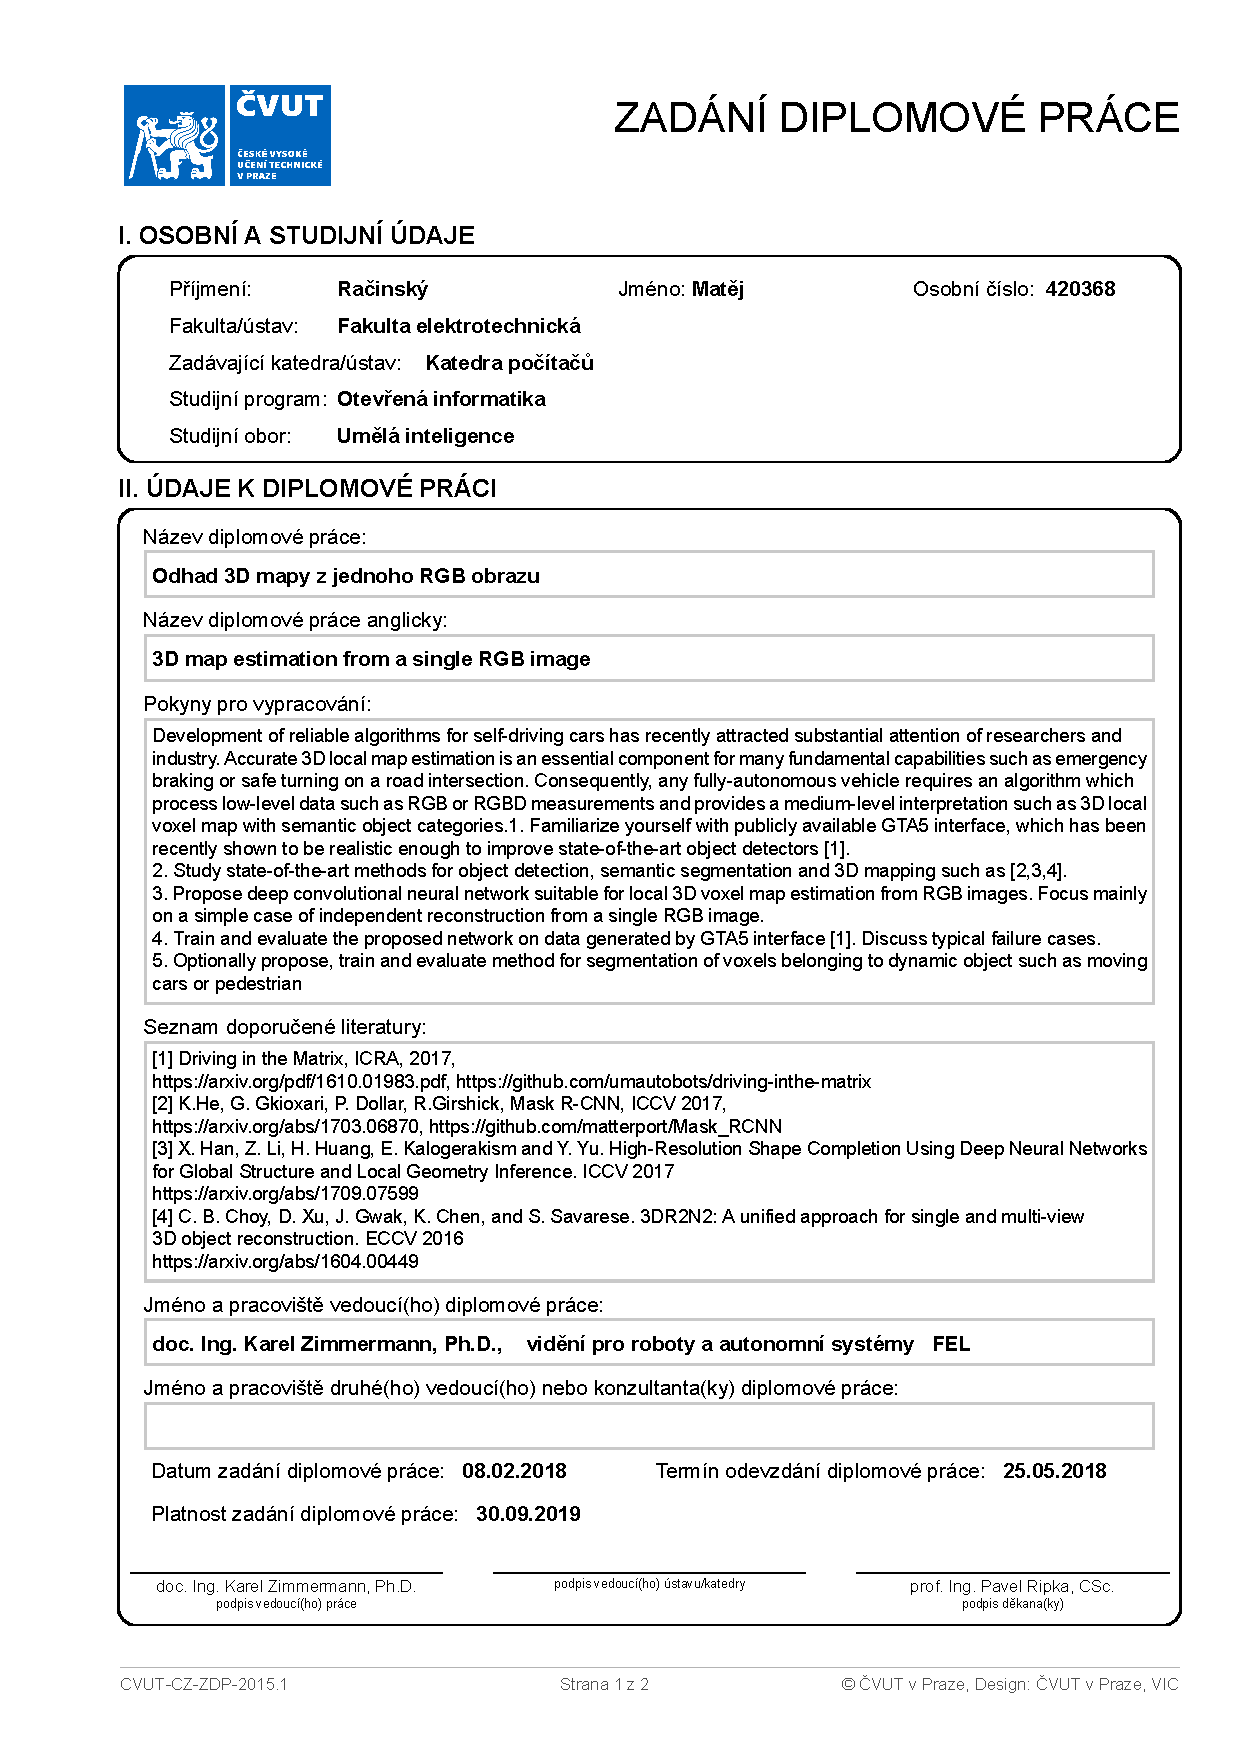
\includepdf[pages=-]{zav_prace_zadani}\thispagestyle{empty}~

{\small{}\ }{\small \par}

\noindent {\small{}\vfill{}
 % nastavuje dynamické umístění následujícího textu do spodní části stránky
~}{\small \par}

\subparagraph*{Author statement for the graduate thesis: \protect \\
}

I declare that the presented work was developed independently and
that I have listed all the sources of information used within it in
accordance with the methodical instructions for observing the ethical
principles in the presentation of university theses. 

{\small{}\bigskip{}
}\noindent {\small{} Prague, date }\_\_\_\_\_\_\_\_{\small{}\hspace{\fill}$\overline{\textrm{~~~~~~~~~signature~~~}}$}\\
{\small{} % doplňte patřičné datum, jméno a příjmení
}{\small \par}

{\small{}%%%   Výtisk pak na tomto míste nezapomeňte PODEPSAT!
%%%                                         *********
}{\small \par}

\cleardoublepage{}

{\small{}\thispagestyle{plain} }{\small \par}

{\small{}%\setcounter{page}{3} % nastavení číslování stránek
}{\small \par}

\noindent {\small{}~\vfill{}
}{\small \par}
\begin{description}
\item [{{\small{}Název~práce:}}] \noindent {\small{}Odhad 3D mapy z jednoho
RGB obrazu}{\small \par}
\item [{{\small{}Autor:}}] \noindent {\small{}Bc. Matěj Račinský}{\small \par}
\item [{{\small{}Katedra~(ústav):}}] \noindent Kate{\small{}dra počítačů}{\small \par}
\item [{{\small{}Abstrakt}}] \noindent Tato práce se zabývá využitím virtuálních
světů z počítačových her jakožto zdroje dat pro strojové učení, a
odhadem voxelové mapy z jednoho RGB obrázku za pomoci hlubokého učení.
Tato práce zahrnuje skripty pro napojení se na PC hru GTA V a sběr
dat z ní pro tvorbu automaticky anotovaných datasetů, a implementaci
hluboké neuronové sítě v TensorFlow. 
\item [{{\small{}Klíčová~slova:}}] \noindent {\small{}Deep learning, Machine
learning, GTA V, virtual world, depth estimation, voxelmap estimation,
RAGE}\\
{\small \par}
\item [{\rule[0.5ex]{1\linewidth}{1pt}}]~{\small \par}
\item [{{\small{}Title:}}] \noindent {\small{}3D map estimation from a
single RGB image}{\small \par}
\item [{{\small{}Author:}}] \noindent {\small{}Bc. Matěj Račinský}{\small \par}
\item [{{\small{}Department:}}] \noindent {\small{}Department of Computer
Science}{\small \par}
\item [{{\small{}Abstract}}] \noindent In this thesis we explore virtual
worlds used as data source for machine learning and voxel map estimation
from single RGB image with deep learning. This thesis describes principles
and implementation of hooking into GTA V and gathering data from it
to create automatically annotated dataset, and implementation of deep
neural network in TensorFlow.
\item [{{\small{}Keywords:}}] \noindent {\small{}Deep learning, Machine
learning, GTA V, virtual world, depth estimation, voxel map estimation,
RAGE}{\small \par}
\end{description}
{\small{}\tableofcontents{}% vkládá automaticky generovaný obsah dokumentu
}{\small \par}

\chapter[Introduction]{Introduction}

The main aim of this thesis is reactive 3D map estimation from single
RGB image. The task of building 3D map is essential procedure in many
robotics tasks and is then utilized in high-level planning. For many
static environments, like buildings and roads, we have detailed maps
available which are being used for this task. But for other environments,
with lots of cars like in parking lots or crossroads, or off-road
trajectories, the pre-calculated 3D map is not available and it needs
to be created online. There are multiple approaches for 3D map estimation,
lots of them using depth measurements. Often used approach is utilization
of depth measurements and then building 3D map which is continuously
updated during movement. This is a complicated task due to matching
newly obtained data on existing 3D map. This thesis describes an approach
based on reactive mapping without the need to build long-term internal
world representation, using only immediate sensor input. Only RGB
camera input is used for 3D map reconstruction instead of depth measurements.
The RGB image has many advantages, RGB cameras are cheap and in higher
resolution than depth sensors. RGB camera is a passive sensor, so
multiple RGB cameras won't interfere with each other unlike LiDARs,
so the RGB image can be obtained easily. Due to the problem of obtaining
dense and precise ground truth, this thesis exploits usage of synthetic
datasets as a fast and efficient way to obtain ground truth for such
task. GTA V is used here as a simulator for the creation of a synthetic
dataset.

\section{Obtaining large annotated datasets for high-capacity models}

In recent years, both machine learning and deep learning has experienced
great progress in many fields \cite{history-began-from-alexnet}.
Deep learning has outperformed many other machine learning approaches
by using deep, high-capacity models trained on large datasets. Especially
in the field of computer vision, neural networks achieve state of
the art results in most of the tasks. Many tasks in computer vision
are the first where deep neural networks achieve state of the art
results before being used in other fields, and in this field, deeper
and deeper architectures are being proposed earlier than in other
fields. With larger amount of parameters, the need for large datasets
is growing, with current datasets unable to cover the need for annotated
data. 

Data has proven to be limiting factor in many computer vision tasks.
The main problem is that manual data annotation is exhausting, time-consuming
and costly. That is even more significant for pixel-wise annotation
which is crucial for tasks of semantic segmentation. Pixel-wise annotated
datasets are orders of magnitude smaller than image classification
datasets. This is sometimes called ``curse of dataset annotation''
\cite{semantic-instance-annotation}, because more detailed semantic
labelling leads to smaller size of dataset. 

Many novel neural network architectures are being proposed every year
because of ongoing research and increasing computing power. With growing
capacity and number of parameters in these new models, there is need
for bigger and bigger datasets for training. Several papers shown
positive correlation between the size of data and performance \cite{unreasonable-effectiveness-of-data,revisiting-unreasonable-efectiveness,real-time-human-pose-recognition-in-parts-from-a-single-depth-image}.

\subsection{Manual annotation services}

There are attempts to develop tooling necessary to speed up the manual
annotation process during datasets creation, most known being the
Amazon Mechanical Turk (AMT) \cite{mechanical-turk} and Supervise.ly
\cite{supervise.ly}.

Amazon Mechanical Turk is a platform for crowdsourcing work and has
been used in many academic fields. AMT is a ``marketplace for work
that requires human intelligence'' \cite{amt-article}, a web-based
platform for distributing tasks to a pool of human workers, known
colloquially as Turkers. These tasks are typically small (i.e. a few
minutes to perform a task rather than days or weeks) and payments
pay task are low, in the orders of cents per task. This platform provides
possibility to distribute the annotation process among many people
at once and for low price. Although still being manual, it accelerates
the annotation process and helps researchers to annotate data more
easily \cite{amt-cv-annotation}. Quality of work can not be guaranteed
since task provider can't supervise workers and correct them manually,
but this disadvantage can be compensated by various quality assurance
approaches \cite{amt-cv-annotation}. Supervise.ly is another web-based
platform, focused on computer vision datasets annotation. It provides
helpful tooling for annotators in unified web interface, speeding
up the annotation process. It offers integration with the AMT, so
together, they seem to be candidate for industrial standard of data
annotation. 

Although these tools lead to faster annotation process at lower cost,
it still can not be compared to the fully automated data gathering
and annotation, which could potentially solve these problems of lack
of datasets in many computer vision and related tasks. The power of
automatic annotation can be also expressed in terms of money. Although
not many manually annotated datasets describe time of annotation,
some of them do. In Cityscapes, the fine annotation took 1.5 hour
per image \cite{cityscapes}. If we had annotators paid minimum hourly
wage in USA, 7.25\$, what would mean each fine annotated image has
price 10.875\$. The whole fine annotated Cityscapes dataset with 5000
images thus have has price at least 54 375\$ and took 312.5 days to
annotate. In the dataset I created as part of my thesis, I gathered
33292 images in 3.5 hours. If we would annotate this dataset same
as Cityscapes fine annotation, it would take over 2080 days, which
is approximately 5.7 years, and it would cost 362 050\$. Now we can
see how this automatic annotation approach is significantly both time
and money saving.

\subsection{Generating synthetic datasets from game engines}

In last decades, gaming industry has grown hugely and expanded from
small and specific community into public society and became mainstream
industry. The gaming industry became big driving force in many fields,
and indirectly influenced even machine learning. The mainstream model
of gaming is on personal computers, where each player has his own
gaming PC, along with console gaming. Thanks to ever-growing number
of players, lots of money got into industry and the growing demand
for better graphics in games led to big improvements in both software-computer
graphics and hardware-graphics cards. With lots of money being invested
by players in their PCs, GPU manufacturers were able to deliver more
powerful GPUs every year and we can see exponential growth of GPU
computational power \cite{high-performance-gpu}.

Big companies in gaming industry have enough resources to develop
the state of the art real-time computer graphics, which can we see
in their products, AAA games with graphics very near to reality. Recent
papers \cite{playing-for-data,driving-in-matrix} have shown that
we can use screenshots from PC games to obtain large automatically
or semi-automatically annotated datasets, which improve learning.
This lets us to outperform same models trained only on real data and
achieve state of the art results on public datasets (KITTI dataset
in \cite{driving-in-matrix} and CamVid dataset in \cite{playing-for-data}).

Other approaches utilizing computer games for machine learning have
appeared recently, one of the most knows being OpenAI Gym, software
platform providing reinforcement learning framework \cite{openai-gym}.
Later, Universe \cite{universe} has been released, designed to turn
various computer games into OpenAI Gym environment, easing to deploy
same reinforcement learning algorithms into many different virtual
worlds, but due to legal issues, they require permission from the
game owner to integrate particular game into the Universe. 

\section{Thesis Contribution}

In this thesis, I propose deep convolutional neural network for 3D
map estimation. For this task, I leverage synthetic data from rich
virtual worlds in form of synthetic dataset and propose software architecture
for dataset creation. Then I create data for training in form of pairs
of RGB image capturing space in front of car, and voxelmap of that
space. In the last part, Then I empirically evaluate multiple setups
of predictions of both depth estimation and 3D map estimation

\subsection{Thesis structure}

This thesis is structured as follows. Chapter 2 covers related work
and previous achievements of synthetic datasets. Chapter 3 describes
game Grand Theft Auto V and its utilization in creating synthetic
datasets, this part serves as a documentation for using libraries
for manipulating the GTA world. Here I describe whole modding process,
the game API, internal game coordinate systems and data which can
be obtained from the game. Chapter 4 describes voxel map estimation
from a single RGB image with network architecture and data preparation.
It is followed by chapter 5, where I describe all experiments done
as part of this thesis. Last chapter contains conclusion of the whole
thesis.

\chapter{Related work}

\section{Using Computer Games for Machine Learning}

Richter et al. \cite{playing-for-data} used GTA V to obtain screenshots
and performed semi-automated pixel-wise semantic segmentation. Although
the process was not fully automatic, the annotation speed per image
was drastically increased, being 771 times faster than fine per-image
annotation of Cityscapes \cite{cityscapes} and 514 times faster than
per-image annotation of CamVid \cite{camvid}. Richter et al. extracted
24 966 images from game GTA V, which is roughly two orders of magnitude
larger than CamVid and three orders of magnitude larger than semantic
annotations for KITTI dataset. They trained the prediction module
of Yu and Kolthun \cite{kolthun-dilation} and by using on $\frac{1}{3}$
of the CamVid training set (which is ) and all 24 966 GTA V screenshots,
they outperformed same model trained on whole CamVid training dataset.

For images extraction, they use RenderDoc\cite{renderdoc}, stand-alone
graphics debugger. It intercepts the communication between the game
and the GPU and allows to gather screenshots. It's advantage is that
it can be used for different games, allowing to gather datasets in
various environments.

Johnson-Roberson et al. \cite{driving-in-matrix} used GTA V screenshots,
depth and stencil buffer to produce car images and automatically calculated
their bounding boxes. 

On these generated data, they trained Faster R-CNN \cite{faster-r-cnn}
only on screenshots from the GTA V game, using up to 200 000 screenshots,
which is one order of magnitude bigger than Cityscapes dataset. Using
only screenshots for training, they outperformed same architecture
trained on Cityscapes, evaluating on KITTI dataset. They developed
their own GTA V mod\ref{sec:GTA-V-modding} to hook into GPU calls
and gather screenshots from here. 

GTA V has also been used as a part of the OpenAI Universe, promising
powerful environment for machine learning, but due to Rockstar Games
Terms of Services, it has been removed and is not currently supported
by the OpenAI Universe. Nowadays, OpenAI Universe supports many games,
but focuses mainly on Reinforcement Learning, and thus allows only
communication with games through a strict API and does not allow the
complex setup and modifications of the game described in this thesis.

\section{3D map estimation}

3D map estimation is a complex an important task in computer vision,
and many approaches have been used in attempts to solve this task.
It is tightly coupled to the depth estimation, because the most important
part of the 3D estimation is to estimate the depth of objects on the
image, since spatial information about horizontal and vertical position
is contained in the image directly. Most studies focus on binocular
cameras \cite{taxonomy-stereo}, also called stereo vision where depth
and 3D map is reconstructed using information from two cameras, and
thus depth and position in 3D can be estimated from seeing same points
from different views. The other approach is to use only single image,
without the binocular information. That task is more challenging due
to lack of information from the second image, and even the State of
the Art approaches fall short compared to the binocular vision. But
thanks to the recent success of deep convolutional neural networks,
there have been advances in monocular depth estimation.

\subsection{Deep convolutional neural networks}

In machine learning, deep convolutional neural networks have been
used more and more mostly due to significant breakthroughs in image
classification tasks. Advantage of deep neural networks is the capability
to naturally utilize low-level, mid-level, and high-level features,
without need for manual feature-engineering and lets us train whole
architectures end-to-end. Recent results \cite{going-deeper-with-convolutions,very-deep-image-recognition}
in visual recognition tasks, mostly on ImageNet dataset \cite{imagenet},
reveal depth of network plays crucial role in model accuracy and started
the revolution in many computer vision tasks \cite{deep-learning-nature}. 

Neural networks are machine learning models vaguely inspired by the
biological neural networks that constitute human brains. Neural networks
are being used as universal approximators, theoretically capable of
arbitrarily accurate approximation to an arbitrary function \cite{universal-approximation}
and thus are used for many different tasks, for instance classification,
regression, clustering, and many other. The neural network, as name
suggests, is network of interconnected artificial neurons. An artificial
neuron is based on biological neuron, but with many simplifications.
It consists of inputs to the neuron (inspired by dendrites), the neuron
itself, and the output of the neuron (inspired by axon). Intuitively
the artificial neuron sums all inputs weighted by neuron weights and
send them to into its activation function, inspired by axon. Formally,
the output of neuron $y$ with inputs $\boldsymbol{x}=\left(x_{0},...,x_{n}\right)$
, weights $\boldsymbol{w}=\left(w_{0},...,w_{n}\right)$, bias $\beta$
and activation function $\varphi\left(\cdot\right)$ is defined as
\[
y=\varphi\left(\beta+\stackrel[i=0]{n}{\sum}w_{i}x_{i}\right)=\varphi\left(\boldsymbol{w}\cdot\boldsymbol{x}+\beta\right)
\]
. In its typical architecture, the neural network comprises of many
layers stacked on top of each other, with output of neurons in one
layer connected to all inputs of all neurons in the next layer and
information flows from each neuron of previous layer to each neuron
of next layer. This is called fully-connected neural network. Other
approach is to connect inputs of a neuron only to a subset of neurons
in previous layers, specifically its corresponding neuron in previous
layer and its neighbours. This dramatically reduces number of parameters
needed to be learned. The neural network is then usually learned end-to-end
by the back-propagation algorithm \cite{backprop} which minimizes
the loss function using stochastic gradient descent or its alternatives.

When neural network has many layers stacked on top of each other,
it is called a deep neural network. The success of deep neural networks
lies in their abilities to approximate non-trivial function because
of high number of parameters of the network. The disadvantage of deep
neural networks is the time they need to learn because it takes days
or weeks to train state of the art deep neural networks. 

\subsection{Residual networks}

As mentioned above, deep network became very popular and widely used
in computer vision and machine learning. But there are some caveats
when building a new deep architecture for neural network. When deeper
networks were created simply by stacking more and more layers in the
model, these models become hard to train. One of these problems is
the notorious vanishing gradient, which is being addressed by many
approaches, like normalized initialization \cite{efficient-backprop,difficulty-deep-forward}
and normalization layers \cite{batch-normalization}. Other problem
is the degradation problem, where training accuracy starts to worsen,
after stacking more layers \cite{highway-networks}. Residual networks
aim to address this problem of degradation.

If shallower model is able to learn with higher accuracy than deeper
model, we want the deeper model to be able to learn at least same
as shallower one, or better. If we stack a new layer into the model,
we want them to be able to learn identity mapping. Then the model
with new layers will behave same as shallower model during prediction.
Experiments show that current solvers using gradient descent are not
able to find such solution which would let newer layer to learn identity
mapping in feasible time. The residual learning aims to tackle this
problem by explicitly learning the residual mapping instead of original
mapping. If we want our newly stacked layers to represent mapping
$\mathcal{H}\left(\boldsymbol{x}\right)$, instead we let them learn
another mapping $\mathcal{F}\left(\boldsymbol{x}\right)=\mathcal{H}\left(\boldsymbol{x}\right)-\boldsymbol{x}$.
The original mapping we aim to, $\mathcal{H}\left(\boldsymbol{x}\right)$
is then reconstructed as $\mathcal{H}\left(\boldsymbol{x}\right)=\mathcal{F}\left(\boldsymbol{x}\right)+\boldsymbol{x}$.
He et al. \cite{resnet} shows it is easier to learn the residual
mapping than to learn the original mapping. It also more easily preserves
the identity mapping, if $\mathcal{F}\left(\boldsymbol{x}\right)=\boldsymbol{0}$,
because it is easier to fit these layers to zero than to explicitly
learn identity mapping. 

The formulation of $\mathcal{F}\left(\boldsymbol{x}\right)+\boldsymbol{x}$
can be realized by feed-forward neural network with shortcut connections
\cite{bishop-neural-networks}, also known as skip connections. The
advantage of this approach is it can be easily implemented in current
neural network frameworks out of the box, and it whole network can
still be learned by SGD end-to-end without any further modifications.
Intuitively, the identity mapping, shortcut connection can be seen
as an information highway, where information flows unchanged both
forwards and backwards without any changes. He et al. \cite{resnet}
show the residual learning lets us train very deep models and present
several architectures based on residual learning: ResNet-18, ResNet-34,
Resnet-50, ResNet-101, and ResNet-152. basically ResNet architecture
consists of 4 residual blocks, repeated many times. The difference
between individual architectures is only in number of repetitions
these residual blocks.
\begin{figure}
\begin{centering}
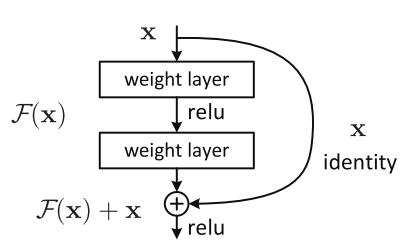
\includegraphics[width=6cm]{obrazky/resnet-layers}
\par\end{centering}
\caption{Residual and shortcut layers\cite{resnet}}
\end{figure}

Residual networks have been widely adopted as a part of many upcoming
architectures for various tasks. Thy are utilized in many image mapping
tasks, for instance depth prediction or semantic segmentation. He
et al. \cite{mask-rcnn} used ResNet as a backbone for their Mask
R-CNN architecture for pixel-wise semantic segmentation and trained
on COCO dataset. Their setup works well on both real photos and synthetic
images, as can be seen in figure \ref{fig:Synthetic-image-labelled}
where image from synthetic dataset is being labelled.

\begin{figure}
\begin{centering}
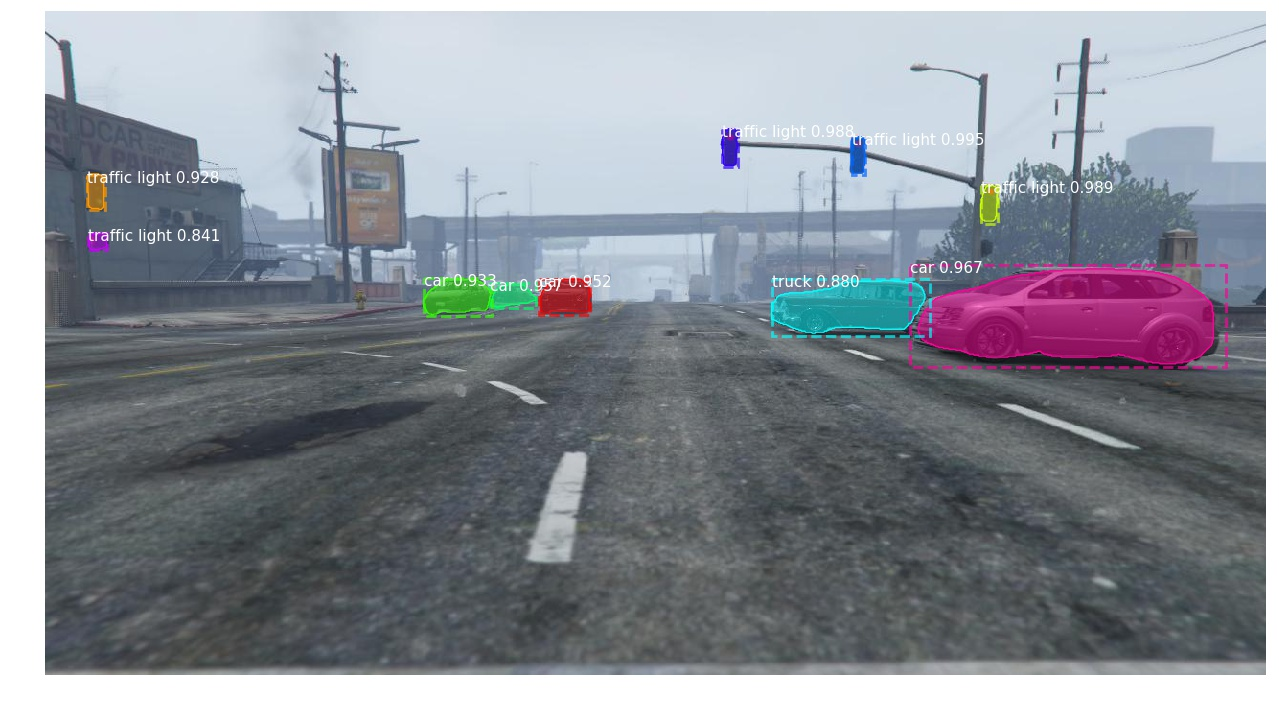
\includegraphics[width=11cm]{obrazky/mask-rcnn}
\par\end{centering}
\caption{\label{fig:Synthetic-image-labelled}Synthetic image labelled by Mask
R-CNN}

\end{figure}


\subsection{Depth estimation}

Depth estimation is one of the most fundamental tasks in computer
vision. Most existing methods \cite{depth-and-surface-estimation,predicting-depth}
formulate depth estimation as a regression task due to the continuous
nature of depth values. Those models for depth estimation are usually
trained to minimize L2 norm between ground truth and predicted depths.
However it shows that regressing to exact depth is difficult task.
In many applications, depth can be known only approximately. With
aforementioned approach, I approximate the regression formulation
of depth estimation with classification problem. Thus instead of training
to predict exact depth, we predict only depth range, still small enough
to be useful for our application. Advantage of classification formulation
of the problem is that after applying softmax on output of neural
network, depths are naturally predicted as confidence in form of probability
that particular depth level is occupied \cite{depth-estimation-as-classification}.
Most notable methods \cite{depth-estimation-as-classification,depth-estimation-hierarchical-fusion-soft-weighting}
use deep convolutional networks based on famous object classification
architectures. 

Li et al. \cite{depth-estimation-hierarchical-fusion-soft-weighting}
use architecture based on deep residual network \cite{resnet}, specifically
Resnet-152. The architecture is modified, it does not use the fully
connected layer in the end of the network, which drastically decreases
the number of trainable parameters, and instead it appends one convolutional
and one deconvolutional layer. Also, Li et al. utilize the hierarchical
fusion, where output of each block of ResNet is concatenated to other
outputs, with dropout layer afterwards, then the network utilizes
both low-level and high-level features of the input image during the
final layers of depth estimation. The output of final layer is 120x160x200,
meaning it outputs 120x160 pixels image with 200 depth levels. The
depth space is equally discretized in log space. Specifically, 
\[
l=round\left(\frac{\log\left(d\right)-\log\left(d_{min}\right)}{q}\right)
\]
where $l$ is the quantized label, q is the width of quantization
bin, $d$ is the continuous depth value and $d_{min}$ is the minimum
depth value in the dataset. 

Other notable approach of Li et al. is soft weighted sum inference.
Usually, the depth is reconstructed intuitively as a centre of depth
bin with maximum value pixel-wise \cite{depth-estimation-as-classification}.
The last layer is softmax, so values can be interpreted as probabilities
of each depth bin being being correct one. Thus the output contains
probability distribution of depth pixel-wise. Li et al. \cite{depth-estimation-hierarchical-fusion-soft-weighting}
reconstruct depth as a soft weighted sum inference by 
\[
\hat{d}=\exp\left\{ \boldsymbol{w}^{T}\boldsymbol{p}\right\} ,w_{i}=\log\left(d_{min}\right)+q\cdot i
\]
where $\boldsymbol{w}$ is the weight vector of depth bins, $i$ is
bin index, $\boldsymbol{p}$ is the output score, and $\hat{d}$ is
reconstructed depth.

Then the model is trained end-to-end to minimize the pixel-wise multinomial
logistic loss 
\begin{equation}
L=-\left[\stackrel[i=1]{N}{\sum}\stackrel[k=1]{K}{\sum}1\left\{ D_{k}=D_{i}^{*}\right\} \log\left(p_{i}^{D_{k}}\right)\right]\label{eq:loss-multinomial}
\end{equation}
where $N$ is the number of pixels, $K$ is the number of depth bins,
$D_{i}^{*}$ is ground truth depth on pixel $i$, and $p_{i}^{D_{k}}$
is the probability of pixel $i$ to be labelled with $D_{k}$ depth
bin.

The classical multi-class classification assumes categorical labels
without any ordering defined. However depth bins are ordinal labels,
not categorical, because they have defined ordering and semantically
it makes sense to take into account distance between correct and predicted
label during training. This approach is not usable for categorical
data, but for nominal data, this knowledge can be used to provide
more information for the learning. Cao et al. \cite{depth-estimation-as-classification}
propose modified loss function which takes distance between depth
ins into account. They use similar architecture, with pixel-wise multinomial
logistic loss, but with slight modification. In usual logistic loss,
the loss is non-zero only for correct label, due to the $1\left\{ D_{k}=D_{i}^{*}\right\} $part
of the function. Cao et al. propose ``information gain'' \cite{depth-estimation-as-classification}
instead, where $1\left\{ D_{k}=D_{i}^{*}\right\} $ is replaced by
$H\left(D_{i}^{*},D_{k}\right)$, where $H$ is $B\times B$ symmetric
matrix with elements $H\left(p,q\right)=exp\left(-\alpha\left(p-q\right)^{2}\right)$
where $\alpha$ is a constant. This information gain matrix lets the
SGD propagate the error not only through correct label and preceding
softmax layer, but also through its neighbouring labels, which helps
updating the network parameters. So the modified loss is 
\begin{equation}
L=-\left[\stackrel[i=1]{N}{\sum}\stackrel[k=1]{K}{\sum}H\left(D_{i}^{*},D_{k}\right)\log\left(p_{i}^{D_{k}}\right)\right]\label{eq:loss-infogain}
\end{equation}
. 

\subsection{3D map estimation}

Choy et al. \cite{choy-3d-r2n2} use an LSTM framework extended for
3D representation reconstruction, called 3D Recurrent Neural Network
for reconstructing 3D images from single or multiple images and perform
State of the Art results on single-view reconstruction. In their setup
they used encoder-decoder architecture with $127\times127$ input
images and $32\times32\times32$ voxelmap and trained it to minimize
the softmax cross-entropy loss. This setup too learns on synthetic
data, using mostly CAD models. This approach is heavily focused on
one object dominating the input image which is suited for precise
3D map estimation, but not much for estimation of 3D map of whole
scene, usually with multiple objects.

\chapter{Transforming GTA V into the State of the Art simulator}

In this thesis, Grand Theft Auto V (GTA V) game is used for creating
synthetic, nearly photo-realistic dataset. 

\section{GTA V introduction}

GTA V is action-adventure open-world video game developed by Rockstar
North and published by Rockstar Games. The game was released on 17.9.2013
for PlayStation 3 and Xbox 360\cite{gta-release} , in 18.11.2014
for PS4 and Xbox One and in 14.4.2015 it was released on PC, Windows\cite{gta-release-pc}.

The game is based on proprietary game engine, called \label{rage}RAGE
(Rockstar Advanced Game Engine) \cite{gta-5-rage}, which is used
as a base for most of Rockstar Games products. 

Till the release on Microsoft, Windows, it has been in development
for 5 years with approximate 1000-person team \cite{gta-interview-studio}.
The world of GTA V was modelled on Los Angeles\cite{gta-v-interview}
and other areas of Southern California, with road networks respecting
design of Los Angeles map. 

As could be expected from AAA game like GTA V, motion capture was
used to character's both body and facial movements. 

There are several reasons why GTA V is better for dataset creation
than other games. To use a game for dataset creation, we have multiple
requirements. The graphics of the game must be near photorealistic,
since we try to to use it instead of photos for computer vision tasks.
This disqualifies most of games, and leaves us only with AAA games
produced by big companies and few other games with State of the Art
graphics. 

The other requirement is possibility of good-enough way to interact
with the game programmatically. Usually we want to setup at least
part of the environment before gathering data. This part heavily depends
on community around the particular game.

Also the advantage of GTA V compared to some other games is abundance
of models and various sceneries in its virtual world. It has complex
transportation system of roads, highways, intersections, railroad
crossing, tunnels, and pedestrians. It also has urban, suburban, and
rural environments \cite{video-games-for-autonomous-driving}.

In gaming subculture, there are communities where people specialize
in reverse-engineering of games and development of modifications to
these games. These people are called modders or mod developers, and
these unofficial modifications and extension of games are called mods.
For few games, developers welcome this kind of activity and sometimes
they even release tools to ease the game modding. In most cases, the
game developers simply don't care and in few cases, they actively
fight against the reverse-engineering and modding. 

The GTA V is second case, where Rockstar Games does not actively try
to prevent the reverse-engineering, but they don't release any tools
to ease it, either. This results in cyclic process of Rockstar Games
releasing new version of game, including backward compatibility (BC)
breaks, and community reverse engineering the new version and adjusting
their mods to work with the new version.

The modding community around the GTA V is based mostly on community
around GTA IV, which was previous big game produced by Rockstar Games.
So many tools are just GTA IV based and only modified to work with
GTA V. Luckily, the community is large and productive, so we have
many mods and many function in GTA V reverse-engineered and thus prepared
for programmatic interactions.

\subsection{Cars}

There is big variety of cars models. Specifically, the are 259 car
models, all of them are listed here \cite{gta-vehicle-models}. These
models cars of various shapes and sizes, from golf carts to trucks
and trailers. This diversity is representative of real distribution
of vehicles. It even allows us to simulate environments with various
types of vehicles, which would be very difficult in real environment.
GTA V provides us many information about cars, more on this will be
covered in section \ref{sec:GTA-V-data-obtaining}.

\subsection{Pedestrians}

GTA V has pedestrians and provides some information about them, more
on this in section \ref{sec:GTA-V-data-obtaining}. The game has pedestrians
of both genders and various ethnicities. Pedestrians appear in various
poses, like standing, walking, sitting, many animations etc. The main
drawback of GTA V is that all pedestrians are about the same height\cite{video-games-for-autonomous-driving}.

\section{Automotive Simulators}

Currently, there are some open-source simulation platforms for automotive
industry which could be theoretically used for creating synthetic
datasets. But compared to AAA games like GTA V, they have much less
resources and much less customers to finance the development. In result,
simulators have worse graphics than AAA games and NPC (non playable
characters) don't have as sophisticated behaviour. In GTA V, drivers
mostly follow traffic regulations, traffic lights and traffic lanes,
which leafs to very realistic environment better than simulators can
provide.

\section{\label{sec:GTA-V-modding}GTA V modding ecosystem}

Although the modding community is quite big, as it is in lots of open-source
communities, essential part of community depends on one person. Here,
it is Alexander Blade. In his free time, he reverse-engineered big
part of GTA V and developed ScriptHookV\cite{scripthookv-gtaforums},
library enabling to perform native calls into GTA V in C++ and develop
GTA V mods in C++. Currently, more people in community participates
in reverse-engineering and they share their knowledge in GTA forum
thread\cite{nativedb-research}.

List of all reverse-engineered native functions is kept in following
list \cite{nativedb}. Assumably, GTA V contains \textasciitilde{}5200
natives. There is no original native name list of functions in GTA
V, name hashes are used instead. During reverse-engineering and game
decompilation, \textasciitilde{}2600 native names were discovered
using brute-force and manual checking afterwards. For these functions,
number of parameters and returns of these calls are also known. In
the native functions list, for big part of functions we know their
name, signature and how do they affect the game. The rest remains
to be discovered yet.

When new version of game is released, in few days to weeks, new version
of ScriptHookV is released, fixing BC breaks.

Other heavily used mod in community is ScriptHookDotNet2, which is
built atop of ScriptHookV and creates bridge between C\# language
and ScriptHookV, effectively allowing to write GTA V mods in C\#.
It is available as open-source \cite{scripthookvdotnet}. Along with
creating bridge between C\# and GTA V, it wraps most used native calls
into classes, leveraging object-oriented paradigm for mod development
using getters and setters as proxies for native calls. 

Next notable mod is NativeUI\cite{nativeui}. It renders windows atop
of GTA V GUI and allows us to define custom control panels for manipulating
custom functionality in other mods. 

Unlike most of other mods, these three mods act more as a framework
for mod development. 

Since GTA V is a game, it requires human interaction. For simulator-like
behaviour we would want the car to drive autonomously to crawl data
without human interaction. This can be done using VAutodrive\cite{vautodrive}.
This allows us to use NPC automatic behaviour patterns for main player,
letting the player randomly wander the world, even in car, without
need of human assistance during crawling. Unfortunately, this package
is not open-source.

Generally, the community is not united in their view on open-source.
Some mods are available open-source on GitHub. Other mods are being
distributed only as compiled binaries\cite{gta-5-mods}. Lots of modders
develop mostly by trial and error, and no comprehensive documentation
for mod development is available, unfortunately. There are some tutorials
\cite{gta-5-mod-tutorial}, but they are far from complete and provide
only basic knowledge, leaving reader without deeper understanding
of underlying principles.

Modders mostly meet online on few GTA forums, where they exchange
knowledge \cite{gta-forums,gta-5-mods-forum}. GitHub or Stack Overflow,
which are biggest information sources for usual software development,
are not used much in GTA modding community. Due to this fact, these
forums, along with source code of open-source mods comprise knowledge-base
of mod development.

\section{Simulation environment and development stack}

In this thesis, I use mod based on \cite{driving-in-matrix} but enhanced
to gain more control of the game and to obtain more information from
the game. 

In later text, I'll refer to some GTA V native functions or data structures
which are output of GTA V native functions. To be consistent and to
help understanding, I will use function names from native function
list \cite{nativedb}.

The basic architecture of C\# mods come from the ScriptHookDotNet2,
where each mod script extends the GTA.Script class. For each child
of this class, we can set integer Interval, Tick and KeyUp callbacks.
Interval property determines how big interval in milliseconds is between
consecutive Tick calls. Tick callback is being called periodically,
so here we can set tasks which we want to perform periodically, e.g.
screenshot gathering. The KeyUp callback is for interacting with user
and reading the user's keyboard input. For data gathering mods, this
is mostly used for debugging purposes, script disabling or restarting. 

The ScriptHookDotNet2 brings useful feature for debugging and developing
scripts based on in. When changing mod compiled binaries, we don't
have to restart the game for newer version of mod to be active. Pressing
Insert causes all C\# binaries to reload, causing new version of source
code to load into game, which dramatically decreases time of feedback
loop during development. This does not work for C++ mods and compiled
.asi files.

During the data retrieval from the game, two types of data are being
gathered. Image data from GPU buffers and data about camera, cars,
pedestrians and other in-game entities. All image data are being persistent
into the filesystem directly. Other data are persisted into PostgreSQL
database running locally on the machine. Since the main mod life-cycle
loop is running in single thread, other threads are used for sending
data into the database for faster simulation. Other setups are possible,
depending on use-case of gathered data and need for scalability. Johnson-Roberson
et al. \cite{driving-in-matrix} send all images into the Amazon Web
Services and save them in a S3 bucket, also the database may run remotely
and since the communication with database runs in separate thread,
longer delay is not an issue. Other approached are saving all data
into the filesystem directly, without database, denormalized per image.
This is easier to setup, but leads to complications during data querying,
because SQL is much more suited querying tool due to the relational
nature of these data.

Since the data retrieval takes many hours usually, there is sometimes
need to change some parameters of the environment without stopping
the run or to generally control the data retrieval remotely. For this
purpose, the mod opens a socket server during startup and reads from
it during the Tick method call. Along with the modded game running,
there is a python REST based web server with simple controls for changing
time of day, weather, stopping and restarting the data retrieval.
During the web server startup, it created socket client which connects
to the socket server in GTA mod. This setup allows to remotely control
the data retrieval over the internet. 

The web-server part with socket client is available on \url{https://github.com/racinmat/GTAVisionExport-Server}.
The installation procedure and running is described in the readme.
It can be run simply by \code{python main.py} which starts the server
on port 5000. It also contains HTML website with server as a client
for the REST API, this can be started either by simply running local
Nginx web-server or by using prepared docker container with properly
configured server. This is run, as usual docker container, by \code{docker compose up}.
The repository also contains lightweight web-based gallery for browsing
gathered images. The main problem with viewing gathered data is their
size. Usually there is hundreds of thousands images (RGB image, depth
image and stencil image per sample) in single directory, which is
difficult to handle for both windows and unix operating systems. To
solve this issue, I developed a lightweight REST API based python
script with pagination support for viewing this dataset. It can be
run by \code{python gallery.py} which starts the REST server on port
5001. The client side of this paginated gallery is in file gallery.html
and also uses the Nginx server to run, same as website for controlling
the data gathering. It uses HTTPS protocol with self-signed certificate,
and the Nginx server is configured to use the HTTP2 protocol which
supports large number of requests at the same time. This bypasses
the restriction of accessing 6 resources at the same time from one
domain which is in HTTP1.1. Thanks to this, hundreds of images can
be displayed in very fast manner, both locally and remotely. The gallery
can be seen in figure \ref{fig:Dataset-viewing-web}.

\begin{figure}
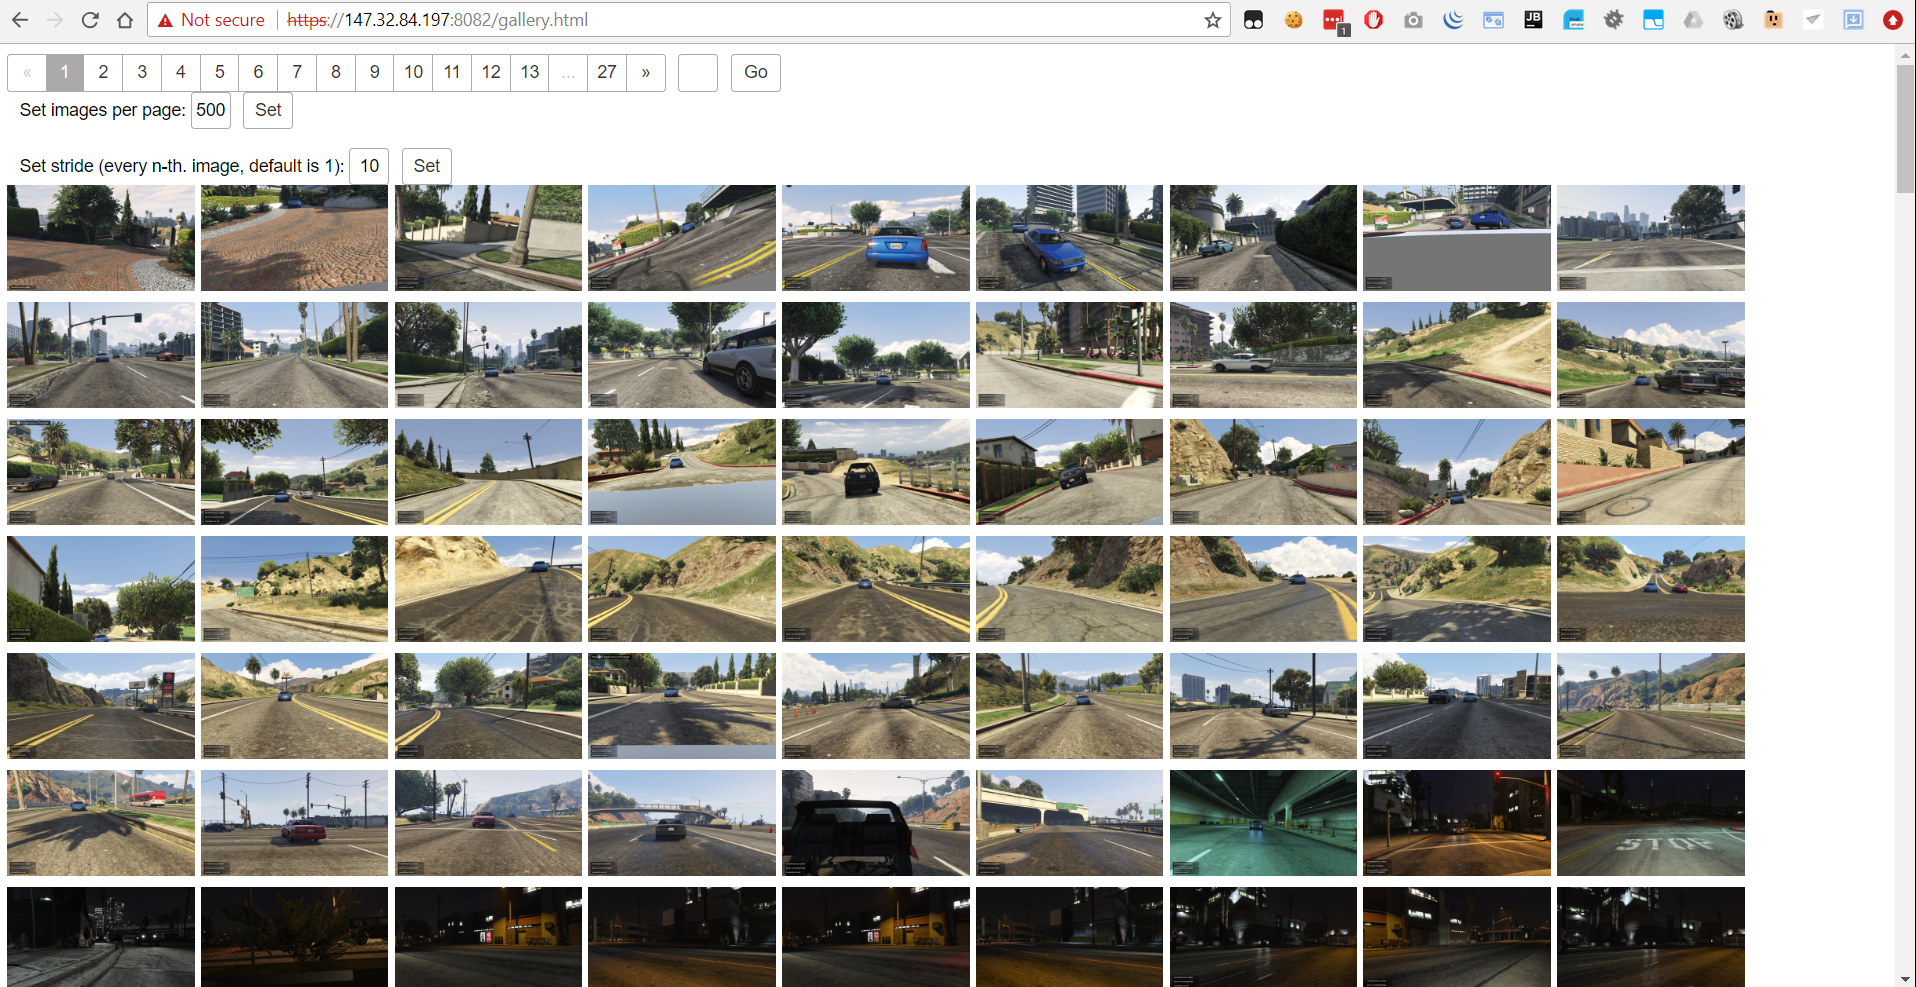
\includegraphics[width=14cm]{obrazky/dataset-viewing.PNG}

\caption{\label{fig:Dataset-viewing-web}Dataset viewing web interface}

\end{figure}


\section{\label{sec:GTA-V-data-obtaining}GTA V native API and data obtaining}

The data obtained from GTA V can be divided into multiple categories.
\begin{itemize}
\item Image data
\item Rendering pipeline matrices
\item GTA V internal data
\begin{itemize}
\item entities
\item camera
\item player
\item other data via API
\end{itemize}
\end{itemize}

\subsection{Image data}

There are 3 image data. RGB image, depth image and stencil image.

RGB image is usual camera image. Depth image is content of GPU's depth
buffer, in NDC. More detailed description of depth values is in subsection
\ref{subsec:Camera-to-NDC}. The last is pixel-wise stencil buffer.
The stencil semantics is explained in the next paragraph.

\subsubsection{Stencil data}

Stencil buffer contains auxiliary data per pixel. It is 8bit unsigned
integer, where 1.-4. bits (counting from LSB) contain object type
ID, and 5.-8. bits contain certain flags. 

That means there are 15 object types and 4 flags. 

For some object type IDs, I reverse engineered its semantics based
on corresponding RGB image. 
\begin{center}
\begin{tabular}{|c|c|c|}
\hline 
Object type ID binary & Object type ID decimal & Semantics\tabularnewline
\hline 
\hline 
0000 & 0 & background (buildings, roads, hills...)\tabularnewline
\hline 
0001 & 1 & pedestrian\tabularnewline
\hline 
0010 & 2 & vehicle\tabularnewline
\hline 
0011 & 3 & tree, grass\tabularnewline
\hline 
0111 & 7 & sky\tabularnewline
\hline 
\end{tabular}
\par\end{center}

The background, pedestrian and vehicle IDs are most important for
vehicles detection and semantic segmentation, and other object types
are not so valuable for these tasks, which is why I didn't investigate
further in semantics and they remain to be reverse-engineered.

For stencil flags, semantics was discovered for half of them. 
\begin{center}
\begin{tabular}{|c|c|c|}
\hline 
position of bit & position in whole stencil value & Semantics\tabularnewline
\hline 
\hline 
5 & xxx1xxxx & artificial light source\tabularnewline
\hline 
8 & 1xxxxxxx & player's character\tabularnewline
\hline 
\end{tabular}
\par\end{center}

Sample stencil image can be seen in \ref{fig:Visualization-pipeline}.
\begin{center}
\begin{figure}
\begin{centering}
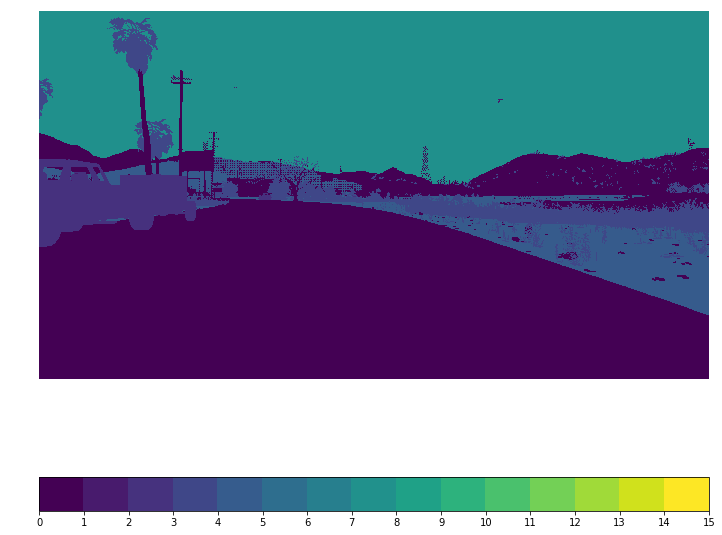
\includegraphics[width=12cm]{obrazky/2018-03-30--06-00-56--114-stencil-color-ids}
\par\end{centering}
\begin{centering}
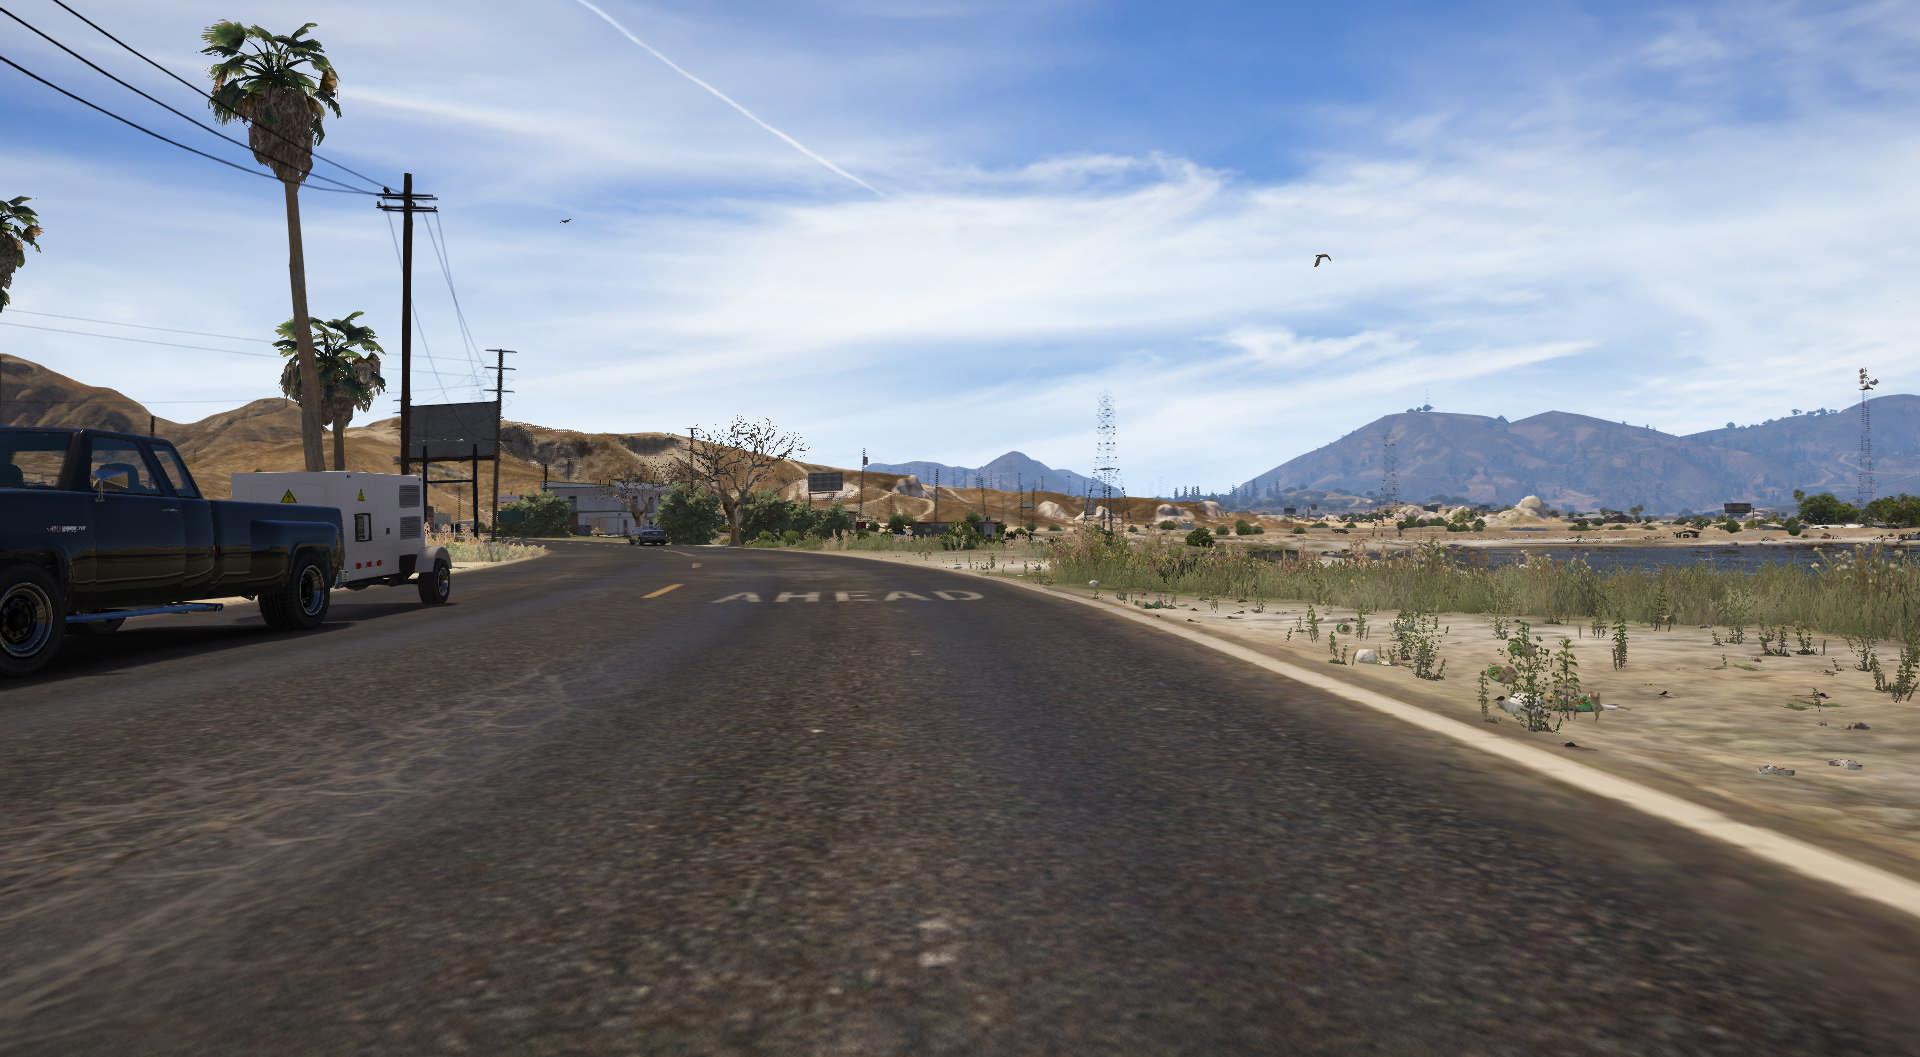
\includegraphics[width=12cm]{obrazky/2018-03-30--06-00-56--114}
\par\end{centering}
\caption{\label{fig:Sample-stencil-object}Sample stencil object types image
and corresponding RGB image}
\end{figure}
\par\end{center}

\subsubsection{Extracting images from GPU's internal buffers}

To understand how the image gathering works, we need to dive deeper
into Microsoft Windows graphics.

In Microsoft Windows, the main graphics engine is DirectX (roughly
Windows equivalent of OpenGL). One part of DirectX is Direct3D, which
is used to render 3D graphics with hardware acceleration, and most
importantly, it provides graphics API. The whole process of obtaining
image data is done by mod provided as part of the paper \cite{driving-in-matrix}.
The mod has two parts, called native and managed plugin.

Image data is being obtained by native plugin by hooking into Direct3D
11's present callback. That means the native call is replaced with
custom code, which is being executed and then returns to the native
call. In that custom code, content of GPU's buffers is copied. Specifically,
the depth and stencil data are captured by hooking into Direct3D’s
ID3D11ImmediateContext:: ClearDepthStencilView and saving the buffers
before each call. Because of optimizations applied by the graphics
card drivers, the function needs to be re-hooked into the clear function
each frame. When saving each sample, the managed plugin requests all
current buffers from the native plugin and the buffers are downloaded
from the GPU and copied into managed memory.\cite{driving-in-matrix}. 

\subsection{\label{subsec:Rendering-pipeline-data}Rendering pipeline data}

Direct3D allows us to get rendering pipelines through the D3D11\_MAP\_READ
call. This way, the world, world-view, and world-view-projection matrices
are obtained. Let's denote them as world matrix = $W$, world-view
by = $VW$, and world-view-projection = $PVW$. We need to get individual
matrices, which we obtain by multiplication by matrices inversion:
\begin{align*}
V & =VW\cdot W^{-1}\\
P & =PVW\cdot\left(VW\right)^{-1}=PV\cdot W^{-1}\cdot V^{-1}
\end{align*}

View and projection matrices are important on their own, without the
world matrix. Their semantics and importance is more described in
section \ref{sec:Reverse-engineering-the-RAGE}. These matrices can
be simply obtained by inversion as stated above. But this approach
is not numerically stable, and sometimes causes resulting matrix to
be incorrect and not usable for further usage. Another caveat of this
approach is that during data gathering in higher speeds, the native
call becomes laggy and resulting matrices are highly imprecise. Although
we can obtain these matrices via the native call, they can be reconstructed
with higher precision, as described in \ref{sec:Reverse-engineering-the-RAGE}.

\subsection{GTA V internal data}

These data are probably most valuable compared to data gathering by
other methods. In this section, I describe which data about various
game objects can be obtained and how to obtain them. 

All data in this section are obtained though native calls into GTA
V, which are listed here \cite{nativedb}. As mentioned above, they
can be called from C++ and C\#. For convenience, and because most
of my mod development is done in C\#, I will also describe the C\#
wrappers. The ScriptHookDotNet2\cite{scripthookvdotnet} wrapper heavily
uses object properties. The C\# API is divided into multiple classes,
listed \href{https://github.com/crosire/scripthookvdotnet/tree/dev_v3/source/scripting}{here}.
Each class has properties, whose getters and setters are implemented
as calling the native functions. This feature is nice tooling and
leads to more readable and maintainable code. I will describe parts
of API which are most useful for synthetic datasets creation.

\subsubsection{Coordinate systems and axes}

The model, world and view coordinate systems are all in meters. In
the model coordinate system, e.g. when we have coordinate system of
a car, Z-axis is oriented upwards, Y-axis is oriented in front of
the car, and X-axis to the right of the car. In the camera coordinate
system, the Z-axis is oriented behind the camera, Y-axis upwards of
camera and the X-axis to the left of camera. In the world coordinate
system, if the camera has rotation = $\left(0,0,0\right)$, it is
heading in direction of Y-axis, X-axis is heading right of the camera,
and Z axis is heading upwards.

\subsubsection{Game state manipulation}

In the ScriptHookVDotNet2, where is Game class, which is the main
entry-point for most of game state manipulation. Here I'll describe
methods and properties useful and needed for data retrieval.
\begin{lyxcode}
Game.Pause(true)
\end{lyxcode}
pauses the whole game. 
\begin{lyxcode}
Game.Pause(false)
\end{lyxcode}
un-pauses the game. The 

\code{Game.ScreenResolution}

property returns Size object with height and width of the current
screen, so 
\begin{lyxcode}
Game.ScreenResolution.Width;~Game.ScreenResolution.Height;
\end{lyxcode}
returns screen width and height respectively. As seen above, the main
player character can be accessed by \code{Game.Player.Character}
property. 

The Player Character property is used for handling the main player.
It has following method important for data retrieval. \code{Game.Player.Character.Position}
provides position of player in world coordinates. This is useful if
we want to obtain entities only in certain distance of player or if
we want to spawn new vehicle on player's position. Similarly to position,
we can access player's current velocity by 
\begin{lyxcode}
Game.Player.Character.Velocity
\end{lyxcode}
which returns the velocity 3D vector. If we have a vehicle, we set
the player as driver as follows 
\begin{lyxcode}
Game.Player.Character.SetIntoVehicle(vehicle,~

VehicleSeat.Driver)
\end{lyxcode}
. When player is in a vehicle, we can access it later by the 
\begin{lyxcode}
Game.Player.Character.CurrentVehicle
\end{lyxcode}
property. 

Other important Class is World, which, as seen above, provides the
camera handling interface, and many other features. As mentioned above,
the World.DestroyAllCameras() clears all scripted cameras. The \code{World.CreateCamera()}
creates new scripted camera. The \code{World.RenderingCamera} holds
reference to the currently active scripted camera. Setting the camera
to the \code{World.RenderingCamera} activates that camera and starts
rendering with that camera, and setting null reference returns the
view to the Gameplay camera, which is default camera used during playing. 

Other methods allow us directly manipulate the world. The \code{World.CurrentDayTime}
returns the TimeSpan object, which is time in day in the GTA world.
By setting this property we can change the time of day as we need
by assigning the TimeSpan instance 
\begin{lyxcode}
World.CurrentDayTime~=~

new~TimeSpan(int~hours,~int~minutes,~int~seconds)
\end{lyxcode}
. The \code{World.Weather} uses same getter, setter interface, so
\code{World.Weather} returns current weather, and \code{World.Weather = Weather.Foggy}
sets the weather to be foggy. List of all possible weathers is in
the Weather enum, which contains Unknown, ExtraSunny, Clear, Clouds,
Smog, Foggy, Overcast, Raining, ThunderStorm, Clearing, Neutral, Snowing,
Blizzard, Snowlight, Christmas, Halloween. 

The World class also contains the 
\begin{lyxcode}
World.CreateVehicle(Model~model,~Vector3~position)
\end{lyxcode}
which spawn new car in the game and returns reference to the newly
spawned car. Position is in world coordinates and model can be any
of vehicle models in game. For instance,
\begin{lyxcode}
World.CreateVehicle(new~Model(VehicleHash.Seven70),~

Game.Player.Character.Position)
\end{lyxcode}
creates new sports car in player's position . Whole list of known
models is available in \url{https://github.com/crosire/scripthookvdotnet/blob/dev_v3/source/scripting/World/Entities/Vehicles/VehicleHash.cs}
where 554 model hashes are enumerated. 

\subsubsection{Camera}

The camera is probably one of the most crucial parts of the API. There
is Gameplay Camera, which is the default camera used during usual
playing. This camera can be manipulated, but its usage is limited.
Other approach is usage of scripted cameras, which can be fully controlled
programmatically. We can create multiple scripted cameras and switch
between them, but the community discovered there is hard limit of
26 cameras at time\cite{gta-mod-camera}. Camera can be created by
calling 
\begin{lyxcode}
Camera~camera~=~World.CreateCamera(

new~Vector3(x,~y,~z),~new~Vector3(x,~y,~z),~float~fov);
\end{lyxcode}
which returns handle to the new camera. The position is in world coordinates
in meters. The rotation is in degrees as rotation around particular
axis, as in OpenGL engine. In the Aircraft principal axes terminology,
the $\left(x,y,z\right)$ rotation vector means $\left(pitch,roll,yaw\right)$
respectively. The fov argument is vertical field of view in degrees.
The default value is 50. One can of course call the underlying native
functions directly, but this wrapper helps with managing the handles. 

All scripted cameras can be destroyed by calling the 
\begin{lyxcode}
World.DestroyAllCameras();~
\end{lyxcode}
Switching to the scripted camera can be done by calling 
\begin{lyxcode}
camera.IsActive~=~true;
\end{lyxcode}
, and switching from this camera to some other by 
\begin{lyxcode}
camera.IsActive~=~false;~
\end{lyxcode}
Right after creating the camera, when we don't to switch to this camera
immediately, we need to deactivate it by these two lines of code
\begin{lyxcode}
camera.IsActive~=~false;

World.RenderingCamera~=~null;
\end{lyxcode}
this code ensures that camera is created properly. We don't know precisely,
why is this needed, but this is the price for using the closed and
reverse-engineered codebase. By calling the
\begin{lyxcode}
camera.IsActive~=~true;~

World.RenderingCamera~=~camera;
\end{lyxcode}
scripted camera becomes active and view is switched to this camera.
All properties of camera can be set simply by calling setters
\begin{lyxcode}
camera.position~=~new~Vector3(x,~y,~z);

camera.rotation~=~new~Vector3(y,~x,~z);

camera.nearClip~=~distance;

camera.farClip~=~distance;

camera.FieldOfView~=~fov;
\end{lyxcode}
and read by calling getters 
\begin{lyxcode}
Vector3~position~=~camera.position;

Vector3~rotation~=~camera.rotation;

float~distance~=~camera.nearClip;

float~distance~=~camera.farClip;

float~fov~=~camera.FieldOfView;
\end{lyxcode}
The near clip and far clip is again in meters. So we can set all needed
parameters simply by calling getters and setters. So if we want to
use camera, we simply set parameters and then activate it. This creates
the static camera. 

Sometimes we want the camera to be moving, e.g. when gathering data
by driving car. Camera can be attached to any entity by calling 
\begin{lyxcode}
camera.AttachTo(entity,~new~Vector3(x,~y,~z));
\end{lyxcode}
the second parameter is relative offset to middle of the attached
entity. The offset is in model coordinate system which means its position
moves and rotates with attached entity. During dataset gathering,
I used this code
\begin{lyxcode}
camera.AttachTo(Game.Player.Character.CurrentVehicle,~

new~Vector3(0f,~2f,~0.4f));
\end{lyxcode}
to attach camera to the front part of player's current vehicle. As
seen from code, it attaches camera 2 meters in front of mar model's
centre and 40cm above it, making it effectively sitting on top of
the hood of the car. These parameters are taken from \cite{video-games-for-autonomous-driving}. 

When we have camera attached to the car, we need to update periodically
its rotation, otherwise it will be heading the same direction in world
coordinates and won't rotate with car it is attached to. So when we
have our Tick method, which is being called periodically, we need
to update the active camera like this:
\begin{lyxcode}
camera.AttachTo(Game.Player.Character.CurrentVehicle,~

cameraPosition);

camera.Rotation~=~cameraRotation;
\end{lyxcode}
if we want to have our camera rotated in fixed offset compared to
car rotation (e.g. camera looking behind the car), we simply set camera's
rotation as offset like this
\begin{lyxcode}
camera.AttachTo(Game.Player.Character.CurrentVehicle,~

new~Vector3(0f,~-2f,~0.6f));~~//~now~our~camera~is~sitting~in~back~of~the~car

camera.Rotation~=~Game.Player.Character.CurrentVehicle.Rotation~

+~new~Vector3(0f,~0f,~180f);
\end{lyxcode}
which sets camera rotation in world coordinates as a sum of car's
rotation and relative rotation of camera, 180\textdegree{} yaw.

\subsubsection{Game entities}

All game entities extend the abstract Entity class. Important children
of Entity class are Ped, Vehicle and Prop classes, wrapping pedestrians,
vehicles, and various objects, respectively. List of all entities
contained in the entity pool can be obtained by \code{World.GetAllEntities()}.
Methods 
\begin{lyxcode}
World.GetAllPeds();~World.GetAllVehicles();~World.GetAllProps();
\end{lyxcode}
will return list of all pedestrians, vehicles, and props, respectively.
These lists are huge and we don't need all of returned entities usually.
Most of the time, we are interested only in objects on the screen,
which are only in certain distance from us. The most straightforward
option is to filter these lists afterwards, but luckily, the library
offers us helper methods for filtering the nearby entities more effectively,
without need to instantiate more distant entities. These helper methods
are 
\begin{lyxcode}
World.GetNearbyEntities(Vector3~position,~float~radius)
\end{lyxcode}
, and analogously, 
\begin{lyxcode}
World.GetNearbyPeds(Vector3~position,~float~radius);~

World.GetNearbyVehicles(Vector3~position,~float~radius);~

World.GetNearbyProps(Vector3~position,~float~radius);
\end{lyxcode}
. As expected, radius is in meters, position is in world coordinates.
So obtaining for instance all vehicles up to half kilometres distant
from the current player, we call 
\begin{lyxcode}
World.GetNearbyVehicles(Game.Player.Character,~500.0f)
\end{lyxcode}
. Every entity has position, rotation, velocity, and handle. Position
and rotation have similar semantics as cameras. Velocity is velocity
as a 3D vector. The handle is unique in-game identifier of particular
entity, allowing identifying it across whole game during data gathering,
and lets us identify same entity on multiple images, which is useful
for identifying motion of entity through different images. By calling
\code{entity.Model.Hash} on a particular entity, we obtain its hash,
which can be used to spawn new entities with same model. For vehicles,
there is \code{entity.ClassType} property, describing type as one
of 21 vehicle types. Whole list can be seen in the enum VehicleClass
in the \url{https://github.com/crosire/scripthookvdotnet/blob/dev_v3/source/scripting/World/Entities/Vehicles/Vehicle.cs}. 

\subsubsection{Gathering data from active camera}

In this part, I'll describe how to access data from internal GPU buffers
and how to persist these data. 

Before we gather buffers contents, we want to pause the game. Since
we don't get the data from buffers perfectly synchronized, we pause
the game to make sure RGB, depth and stencil buffer contain data coming
from same frame. \code{Game.Pause(true)} pauses the game. The whole
data retrieval from buffers is done via GTAVisionExport native plugin
\cite{driving-in-matrix}. When the game is stopped, we can obtain
RGB, depth and stencil buffer contents by 
\begin{lyxcode}
var~color~=~VisionNative.GetColorBuffer();

var~depth~=~VisionNative.GetDepthBuffer();

var~stencil~=~VisionNative.GetStencilBuffer();~
\end{lyxcode}
and then, we save it to the filesystem as TIFF image. Although TIFF
is not the most used format for data, it is able to persist image
whose pixels contain float values, which is crucial for depth buffer.

The RGB buffer is usual 8bit unsigned integer RGBA image. The depth
buffer contains float values, with 32bits precision, in range from
0 to 1, representing depth value in NDC space. The stencil buffer
contains 8bit unsigned integer image. 

\section{\label{sec:Reverse-engineering-the-RAGE}Reverse-engineering the
RAGE rendering pipeline}

As mentioned above \ref{rage}, GTA V uses proprietary game engine,
Rockstar Advanced Game Engine (RAGE). The basic premise of rendering
pipeline is same as in well known graphics engines like OpenGL. The
pipeline is shown in figure \ref{fig:Visualization-pipeline}. Following
section will be discussing mostly computer graphics related problems.
Due to some terminology inconsistency between computer graphics and
computer vision, all terms used here will be computer graphics related.
Probably most confusion here could be caused by projection matrix.
In computer vision, projection matrix is projection from 3D to 2D,
the matrix reduces dimension. In computer graphics, all coordinates
are kept in 4D, in homogeneous coordinates as long as possible. Here
the projection matrix represents projection from frustum seen by eye
into cuboid space of Normalized Device Coordinates.

\begin{figure}
\begin{centering}
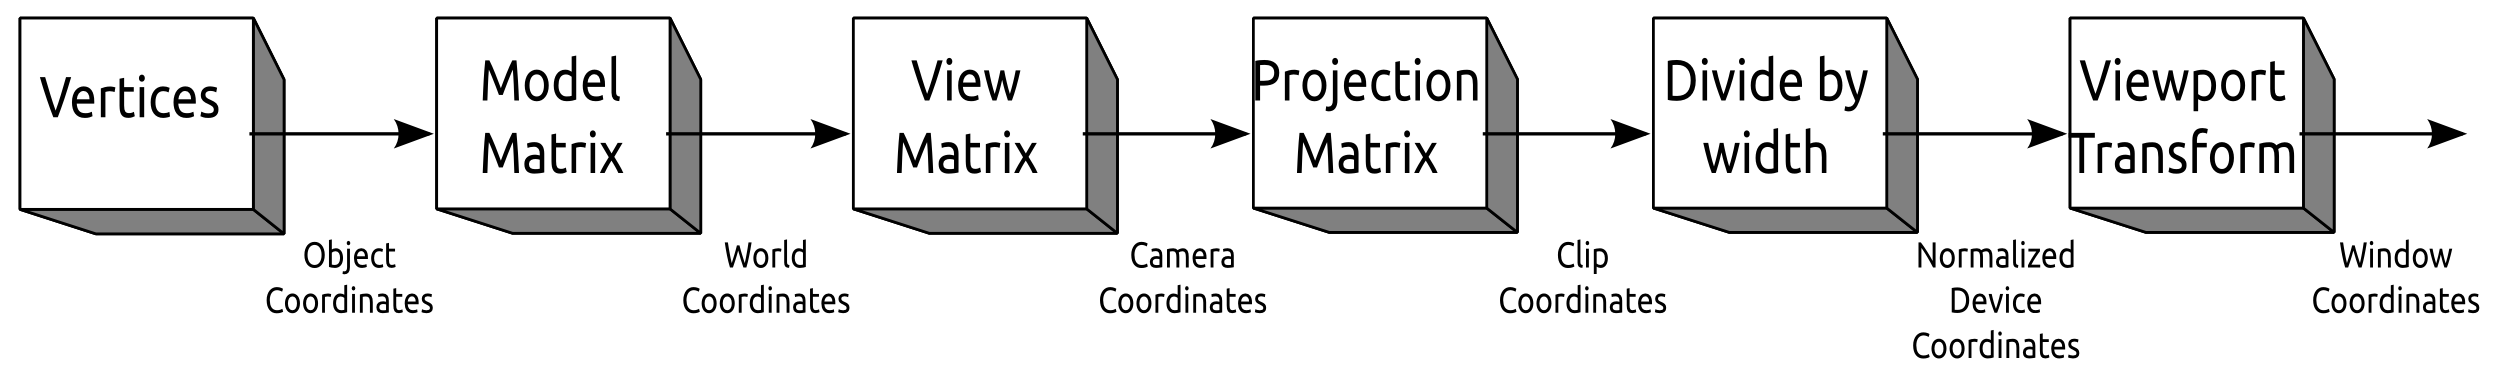
\includegraphics[scale=0.65]{obrazky/transformationPipeline}
\par\end{centering}
\caption{\label{fig:Visualization-pipeline}Rendering pipeline}
\end{figure}
In is part, I will describe some transformations between individual
RAGE coordinate systems. Some points here will have part of name in
lower index. The name of coordinate system will be denoted in upper
index. In RAGE there are 6 coordinate systems.
\begin{center}
\begin{tabular}{|c|c|c|}
\hline 
Name & Abbreviation & Example point $x$\tabularnewline
\hline 
\hline 
Object Coordinates & O & $x^{O}$\tabularnewline
\hline 
World Coordinates & W & $x^{W}$\tabularnewline
\hline 
Camera Coordinates & C & $x^{C}$\tabularnewline
\hline 
Clip Coordinates & L & $x^{L}$\tabularnewline
\hline 
Normalized Device Coordinates & NDC & $x^{NDC}$\tabularnewline
\hline 
Windows Coordinates & P & $x^{P}$\tabularnewline
\hline 
\end{tabular}
\par\end{center}

Most of points we handle in GTA already are in world coordinates. 

But some points, like GAMEPLAY::GET\_MODEL\_DIMENSIONS

$=\begin{pmatrix}x_{max}^{O} & y_{max}^{O} & z_{max}^{O}\end{pmatrix}\begin{pmatrix}x_{min}^{O} & y_{min}^{O} & z_{min}^{O}\end{pmatrix}$
output, are in object coordinates. Transitions between adjacent coordinate
systems will be demonstrated on model dimensions because it is on
the few vectors which are obtained in Object Coordinates and there
is need to project them into Window Coordinates.

\subsection{Object to World Coordinates}

To get world coordinates of model dimensions, we use traditional rigid
body transformation based on ENTITY::GET\_ENTITY\_ROTATION$=\begin{pmatrix}\alpha & \beta & \gamma\end{pmatrix}$
Euler angles, 

and ENTITY::GET\_ENTITY\_COORDS$=\begin{pmatrix}x^{W} & y^{W} & z^{W}\end{pmatrix}$.

Because all coordinates will be homogeneous coordinates, the above-mentioned
model dimensions vectors will be transformed to following form $\begin{pmatrix}x_{max}^{O} & y_{max}^{O} & z_{max}^{O} & 1\end{pmatrix}\begin{pmatrix}x_{min}^{O} & y_{min}^{O} & z_{min}^{O} & 1\end{pmatrix}$. 

The transition is represented by model matrix
\begin{align*}
M & =\begin{bmatrix}1 & 0 & 0 & x^{W}\\
0 & 1 & 0 & y^{W}\\
0 & 0 & 1 & z^{W}\\
0 & 0 & 0 & 1
\end{bmatrix}\begin{bmatrix}1 & 0 & 0 & 0\\
0 & \cos\left(\alpha\right) & -\sin\left(\alpha\right) & 0\\
0 & \sin\left(\alpha\right) & \cos\left(\alpha\right) & 0\\
0 & 0 & 0 & 1
\end{bmatrix}\begin{bmatrix}\cos\left(\beta\right) & 0 & \sin\left(\beta\right) & 0\\
0 & 1 & 0 & 0\\
-\sin\left(\beta\right) & 0 & \cos\left(\beta\right) & 0\\
0 & 0 & 0 & 1
\end{bmatrix}\begin{bmatrix}\cos\left(\gamma\right) & -\sin\left(\gamma\right) & 0 & 0\\
\sin\left(\gamma\right) & \cos\left(\gamma\right) & 0 & 0\\
0 & 0 & 1 & 0\\
0 & 0 & 0 & 1
\end{bmatrix}\\
 & =\begin{bmatrix}\cos\left(\beta\right)\cos\left(\gamma\right) & -\cos\left(\beta\right)\sin\left(\gamma\right) & \sin\left(\beta\right) & x^{W}\\
\sin\left(\alpha\right)\sin\left(\beta\right)\cos\left(\gamma\right)+\cos\left(\alpha\right)\sin\left(\gamma\right) & \cos\left(\alpha\right)\cos\left(\gamma\right)-\sin\left(\alpha\right)\sin\left(\beta\right)\sin\left(\gamma\right) & -\sin\left(\alpha\right)\cos\left(\beta\right) & y^{W}\\
\sin\left(\alpha\right)\sin\left(\gamma\right)-\cos\left(\alpha\right)\sin\left(\beta\right)\cos\left(\gamma\right) & \cos\left(\alpha\right)\sin\left(\beta\right)\sin\left(\gamma\right)+\sin\left(\alpha\right)\cos\left(\gamma\right) & \cos\left(\alpha\right)\cos\left(\beta\right) & z^{W}\\
0 & 0 & 0 & 1
\end{bmatrix}
\end{align*}

and whole transformation is, as expected 
\[
M\begin{bmatrix}x_{max}^{O} & x_{min}^{O}\\
y_{max}^{O} & y_{min}^{O}\\
z_{max}^{O} & z_{min}^{O}\\
1 & 1
\end{bmatrix}=\begin{bmatrix}x_{max}^{W} & x_{min}^{W}\\
y_{max}^{W} & y_{min}^{W}\\
z_{max}^{W} & z_{min}^{W}\\
w_{max}^{W} & w_{min}^{W}
\end{bmatrix}
\]


\subsection{\label{subsec:World-to-Camera}World to Camera Coordinates}

The transformation from world coordinates is principally the same,
but counter-intuitive in definition of used rotation matrices. It
also is rigid body transformation, but rotation is defined differently
than we are usually used to in computer graphics. The rotation matrices
were reverse engineered as part of this thesis from camera position,
rotation and resulting view matrix, this coordinate system is nowhere
else documented. The camera position is CAM::GET\_CAM\_COORD$=\begin{pmatrix}x^{W} & y^{W} & z^{W}\end{pmatrix}$
and the camera rotation is CAM::GET\_CAM\_ROT$=\begin{pmatrix}\alpha & \beta & \gamma\end{pmatrix}$.

The transformation is represented by view matrix
\begin{align*}
V & =\begin{bmatrix}1 & 0 & 0 & 0\\
0 & \sin\left(\alpha\right) & \cos\left(\alpha\right) & 0\\
0 & \cos\left(\alpha\right) & -\sin\left(\alpha\right) & 0\\
0 & 0 & 0 & 1
\end{bmatrix}\begin{bmatrix}\cos\left(\beta\right) & 0 & -\sin\left(\beta\right) & 0\\
0 & 1 & 0 & 0\\
\sin\left(\beta\right) & 0 & \cos\left(\beta\right) & 0\\
0 & 0 & 0 & 1
\end{bmatrix}\begin{bmatrix}\cos\left(\gamma\right) & \sin\left(\gamma\right) & 0 & 0\\
\sin\left(\gamma\right) & -\cos\left(\gamma\right) & 0 & 0\\
0 & 0 & 1 & 0\\
0 & 0 & 0 & 1
\end{bmatrix}\begin{bmatrix}1 & 0 & 0 & x^{W}\\
0 & 1 & 0 & y^{W}\\
0 & 0 & 1 & z^{W}\\
0 & 0 & 0 & 1
\end{bmatrix}
\end{align*}
to fit the matrix into page, let us propose following substitutions 

\[
\cos\left(\alpha\right)=c_{\alpha},sin\left(\alpha\right)=s_{\alpha}
\]

\[
\cos\left(\beta\right)=c_{\beta},sin\left(\beta\right)=s_{\beta}
\]

\[
\cos\left(\gamma\right)=c_{\gamma},sin\left(\gamma\right)=s_{\gamma}
\]
\begin{align}
V & =\begin{bmatrix}c_{\beta}c_{\gamma} & c_{\beta}s_{\gamma} & -s_{\beta} & 0\\
c_{\alpha}s_{\beta}c_{\gamma}+s_{\alpha}s_{\gamma} & c_{\alpha}s_{\beta}s_{\gamma}-s_{\alpha}c_{\gamma} & c_{\alpha}c_{\beta} & 0\\
c_{\alpha}s_{\gamma}-s_{\alpha}s_{\beta}c_{\gamma} & -s_{\alpha}s_{\beta}s_{\gamma}-c_{\alpha}c_{\gamma} & -s_{\alpha}c_{\beta} & 0\\
0 & 0 & 0 & 1
\end{bmatrix}\begin{bmatrix}1 & 0 & 0 & x^{W}\\
0 & 1 & 0 & y^{W}\\
0 & 0 & 1 & z^{W}\\
0 & 0 & 0 & 1
\end{bmatrix}\nonumber \\
 & =\begin{bmatrix}c_{\beta}c_{\gamma} & c_{\beta}s_{\gamma} & -s_{\beta} & x^{W}c_{\beta}c_{\gamma}+y^{W}c_{\beta}s_{\gamma}-z^{W}s_{\beta}\\
c_{\alpha}s_{\beta}c_{\gamma}+s_{\alpha}s_{\gamma} & c_{\alpha}s_{\beta}s_{\gamma}-s_{\alpha}c_{\gamma} & c_{\alpha}c_{\beta} & x^{W}\left(c_{\alpha}s_{\beta}c_{\gamma}+s_{\alpha}s_{\gamma}\right)+y^{W}\left(c_{\alpha}s_{\beta}s_{\gamma}-s_{\alpha}c_{\gamma}\right)+z^{W}c_{\alpha}c_{\beta}\\
c_{\alpha}s_{\gamma}-s_{\alpha}s_{\beta}c_{\gamma} & -s_{\alpha}s_{\beta}s_{\gamma}-c_{\alpha}c_{\gamma} & -s_{\alpha}c_{\beta} & x^{W}\left(c_{\alpha}s_{\gamma}-s_{\alpha}s_{\beta}c_{\gamma}\right)+y^{W}\left(-s_{\alpha}s_{\beta}s_{\gamma}-c_{\alpha}c_{\gamma}\right)-z^{W}s_{\alpha}c_{\beta}\\
0 & 0 & 0 & 1
\end{bmatrix}\label{eq:camera-m}
\end{align}

and whole transformation is, as expected 
\[
V\begin{bmatrix}x_{max}^{W} & x_{min}^{W}\\
y_{max}^{W} & y_{min}^{W}\\
z_{max}^{W} & z_{min}^{W}\\
w_{max}^{W} & w_{min}^{W}
\end{bmatrix}=\begin{bmatrix}x_{max}^{C} & x_{min}^{C}\\
y_{max}^{C} & y_{min}^{C}\\
z_{max}^{C} & z_{min}^{C}\\
w_{max}^{C} & w_{min}^{C}
\end{bmatrix}
\]

From definition of rotation axes in the rotation matrices, following
observation can be made. $z^{C}$ represents distance from camera
in direction of camera heading, and $x^{C}$and $y^{C}$ represent
horizontal and vertical position of point relative to camera, respectively.
But the view frustum of camera is in opposite direction than $z^{C}$axis,
which means the camera ``is looking'' into negative $z^{C}$ coordinates.

\subsection{\label{subsec:Camera-to-NDC}Camera to NDC}

This is the first transformation which is not rigid-body transformation.
Because camera sees only frustum, this transformation represents transition
from frustum to cuboid in Normalized Device Coordinates. The frustum
being projected is specified by near clip, far clip, field of view
and screen resolution width and height. Usually, none of these parameters
are changing during the game, so the projection matrix is usually
the same for multiple scenes during data gathering session. Although
all of these parameters can be changed programmatically if needed. 

The near clip and far clip of camera can be obtained by \label{native-call-near-clip}
CAM::GET\_CAM\_NEAR\_CLIP$=n_{c}$ and CAM::GET\_CAM\_FAR\_CLIP$=f_{c}$.
Width and height of screen resolution are obtained by GRAPHICS::\_GET\_ACTIVE\_SCREEN\_RESOLUTION$=\begin{pmatrix}W & H\end{pmatrix}$
and field of view of camera by CAM::GET\_CAM\_FOV$=\varphi_{VD}$
in degrees. $\varphi_{VD}$ in radians will be denoted as $\varphi_{VR}$.

The near clip and far clip define planes between which the content
is being rendered. Nothing before the near clip and behind the far
clip is rendered.

The field of view $\varphi_{VD}$ is only vertical. Horizontal field
of view can be calculated from $W$ and $H$ ratio, but currently
we don't need it.

There is important observation, the far clip $f_{c}$ does not figure
in the projection matrix at all. In the projection matrix, only $n_{c}$
is used. Far clip used in projection matrix is non-changing value
which can not be obtained through Camera native function. By reverse-engineering
I calculated the value of this new far clip to be $10003.815$, details
of this calculation are covered in experiments\ref{subsec:Reverse-engineering}. 

The transformation is represented by projection matrix
\begin{align}
P & =\begin{bmatrix}\frac{H}{W\cdot\tan\left(\frac{\varphi_{VR}}{2}\right)} & 0 & 0 & 0\\
0 & \frac{1}{\tan\left(\frac{\varphi_{VR}}{2}\right)} & 0 & 0\\
0 & 0 & \frac{-10003.815}{n_{c}-10003.815} & \frac{-10003.815\cdot n_{c}}{n_{c}-10003.815}\\
0 & 0 & -1 & 0
\end{bmatrix}\label{eq:projection-m}
\end{align}

So the projection to Clip Coordinates is 
\[
P\begin{bmatrix}x_{max}^{C} & x_{min}^{C}\\
y_{max}^{C} & y_{min}^{C}\\
z_{max}^{C} & z_{min}^{C}\\
w_{max}^{C} & w_{min}^{C}
\end{bmatrix}=\begin{bmatrix}x_{max}^{L} & x_{min}^{L}\\
y_{max}^{L} & y_{min}^{L}\\
z_{max}^{L} & z_{min}^{L}\\
w_{max}^{L} & w_{min}^{L}
\end{bmatrix}
\]

The transition between Clip Coordinates and NDC is only division by
width, so it is

\[
\begin{bmatrix}x_{max}^{L} & x_{min}^{L}\\
y_{max}^{L} & y_{min}^{L}\\
z_{max}^{L} & z_{min}^{L}\\
w_{max}^{L} & w_{min}^{L}
\end{bmatrix}\circ\begin{bmatrix}\frac{1}{w_{max}^{L}} & \frac{1}{w_{min}^{L}}\\
\frac{1}{w_{max}^{L}} & \frac{1}{w_{min}^{L}}\\
\frac{1}{w_{max}^{L}} & \frac{1}{w_{min}^{L}}\\
\frac{1}{w_{max}^{L}} & \frac{1}{w_{min}^{L}}
\end{bmatrix}=\begin{bmatrix}x_{max}^{NDC} & x_{min}^{NDC}\\
y_{max}^{NDC} & y_{min}^{NDC}\\
z_{max}^{NDC} & z_{min}^{NDC}\\
1 & 1
\end{bmatrix}
\]
where $\circ$ is Hadamard product, also known as entry-wise product
or element-wise matrix multiplication. 

Let us have vector $\boldsymbol{x}=\begin{bmatrix}x & y & z & w\end{bmatrix}^{T}$in
both coordinate systems, $\boldsymbol{x}^{L}=\begin{bmatrix}x^{L} & y^{L} & z^{L} & w^{L}\end{bmatrix}^{T}$,
$\boldsymbol{x}^{NDC}=\begin{bmatrix}x^{NDC} & y^{NDC} & z^{NDC} & w^{NDC}\end{bmatrix}^{T}$.
Then, the relation between Clip Coordinates and NDC can also be expressed
by following relationship 
\[
\boldsymbol{x}^{L}=\begin{bmatrix}x^{L}\\
y^{L}\\
z^{L}\\
w^{L}
\end{bmatrix}=\begin{bmatrix}x^{NDC}w^{L}\\
y^{NDC}w^{L}\\
z^{NDC}w^{L}\\
w^{L}
\end{bmatrix}=w^{L}\begin{bmatrix}x^{NDC}\\
y^{NDC}\\
z^{NDC}\\
1
\end{bmatrix}=w^{L}\boldsymbol{x}^{NDC}
\]

The view frustum was now transformed into NDC cuboid. The NDC cuboid
has dimensions $x\in\left[-1,1\right],y\in\left[-1,1\right],z\in\left[0,1\right]$.
The x and y coordinates are intuitive, but the z-axis is reverted,
so near clip is being mapped to 1 and far clip is being mapped to
0. The NDC is important because it is coordinate space in which GPU
operates and depth is gathered from GPU in NDC. The value of $z^{NDC}=0$
usually belongs to sky.

The camera divides the camera space to two half-spaces, in front of
camera $z^{C}<0$, and behind camera $z^{C}\geq0$ . The projection
transformation from camera space to NDC space works correctly only
for points that belong to half-space $z^{C}<0$. For every point in
camera space, we can easily verify to which half-space it belongs
and project only points belonging to the $z^{C}<0$ half-space. If
we project points behind the camera,$z^{C}\geq0$ to the NDC space,
they will be mapped into the NDC space as if they were in front of
camera.

\subsection{NDC to Window Coordinates}

This is the last transformation of the rendering pipeline and only
in this transformation the dimension reduction happen. So far points
have been kept in homogeneous coordinates, but window coordinates
are only 2D, expressing $x$ and $y$ coordinates of pixel where point
will be rendered. Here, we need only GRAPHICS::\_GET\_ACTIVE\_SCREEN\_RESOLUTION$=\begin{pmatrix}W & H\end{pmatrix}$
because this transformation depends only on screen with and height. 

The transformation matrix is 
\begin{align*}
T & =\begin{bmatrix}\frac{W}{2} & 0 & 0 & \frac{W}{2}\\
0 & \frac{-H}{2} & 0 & \frac{H}{2}
\end{bmatrix}
\end{align*}

so the NDC to screen transformation is
\[
T\begin{bmatrix}x_{max}^{NDC} & x_{min}^{NDC}\\
y_{max}^{NDC} & y_{min}^{NDC}\\
z_{max}^{NDC} & z_{min}^{NDC}\\
1 & 1
\end{bmatrix}=\begin{bmatrix}x_{max}^{P} & x_{min}^{P}\\
y_{max}^{P} & y_{min}^{P}
\end{bmatrix}
\]

Due to the division by width, the pipeline unfortunately can not be
expressed as matrix multiplication by matrix constant for all points
in one scene. 

\section{\label{sec:Datasets-proposal}VirtualScapes Dataset proposal}

As part of my thesis, I propose two novel synthetic datasets. Both
of these datasets are outdoor, taken from virtual car. Both of these
datasets contain outdoor images in all parts of day, dawn, day, evening,
and night. They contain most of data described above, to provide as
much information as possible for usability in various tasks. Both
of these datasets contain full HD RGB-D images, stencil images, position
and rotation of camera, positions, rotations, identifiers and types
of cars and pedestrians around the camera, projection and view matrix
for aligning data between different images. 

The first dataset, named Closed VirtualScapes, was used for voxel
map reconstruction. It contains images from 4 virtual cameras attached
to driving car, placed in circle opposite to each other, mapping space
in front of car to create its detailed 3D reconstruction. There are
8371 scenes, each taken from 4 cameras. During this dataset gathering,
$13059$ meters were driven in virtual world.

The second dataset, named Open VirtualScapes, is demonstration of
common automotive dataset from driving car. Compared to real-world
datasets, this one has advantage of pixel-wise depth, precise on all
surfaces and even in high distances, outperforming LiDAR technology
in accuracy and depth point density. It is directly aligned with pixels
of RGB images. The datasets consists of 22285 scenes, every of them
captured by 4 cameras attached to car, heading different direction,
as seen in figure \ref{fig:Camera-positions-for} where camera positions
are marked by white cubes. During this dataset gathering, $34340$
meters were driven in virtual world. Both datasets are publicly available
and can be downloaded from \url{http://ptak.felk.cvut.cz/public_datasets/GTA_V/dataset-website/}. 

To demonstrate possibilities of synthetic, automatically annotated
datasets, here are some sample images obtained using my data extraction
described in \ref{sec:GTA-V-data-obtaining} . The dataset contains
position, rotation, model sizes, identifier and the pixel-wise class
segmentation of each car. With this data, I was able to do the 3D
and 2D bounding boxes extraction, pixel-wise object segmentation and
trajectory tracking. All of these images are part of the VirtualScapes
dataset and can be automatically reconstructed using annotations included
in dataset.

\begin{figure}
\begin{centering}
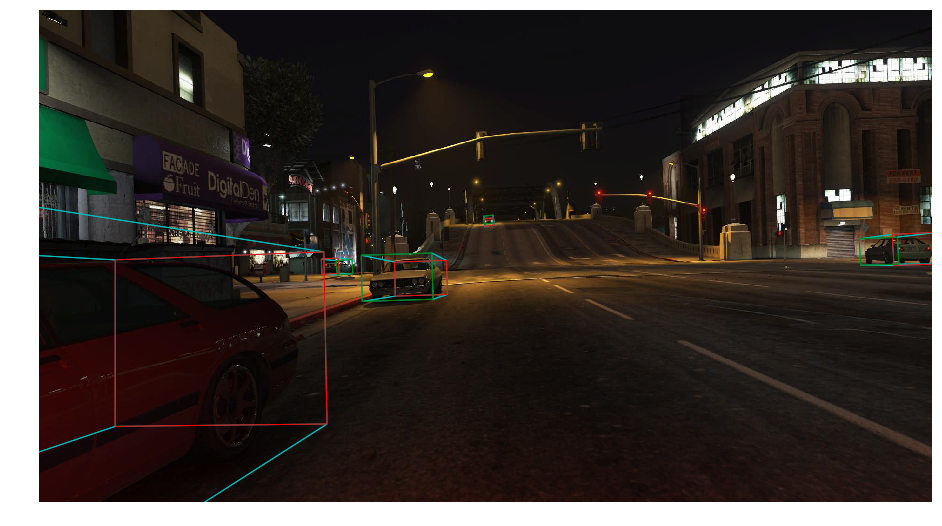
\includegraphics[width=12cm]{obrazky/bbox-night}
\par\end{centering}
\caption{3D bounding box - night}
\end{figure}
\begin{figure}
\begin{centering}
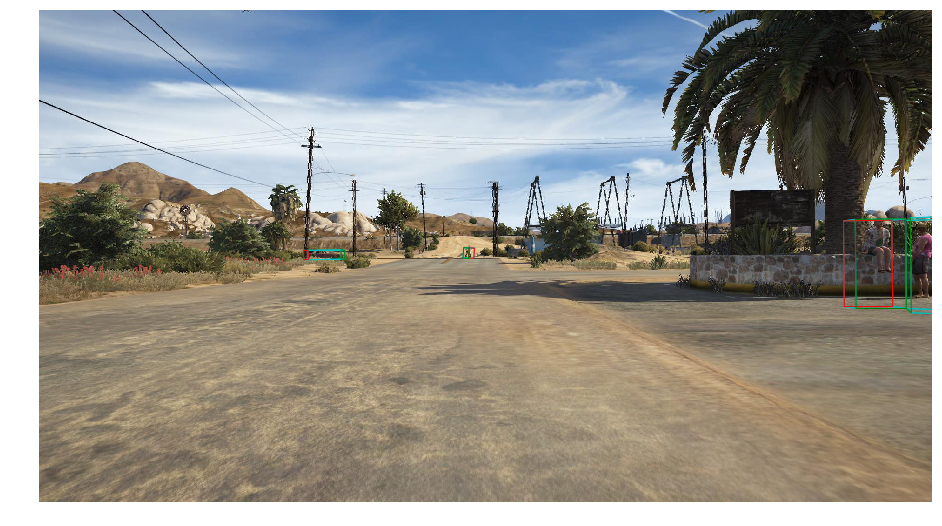
\includegraphics[width=12cm]{obrazky/bbox-day-people}
\par\end{centering}
\caption{3D bounding box - day}
\end{figure}
\begin{figure}
\begin{centering}
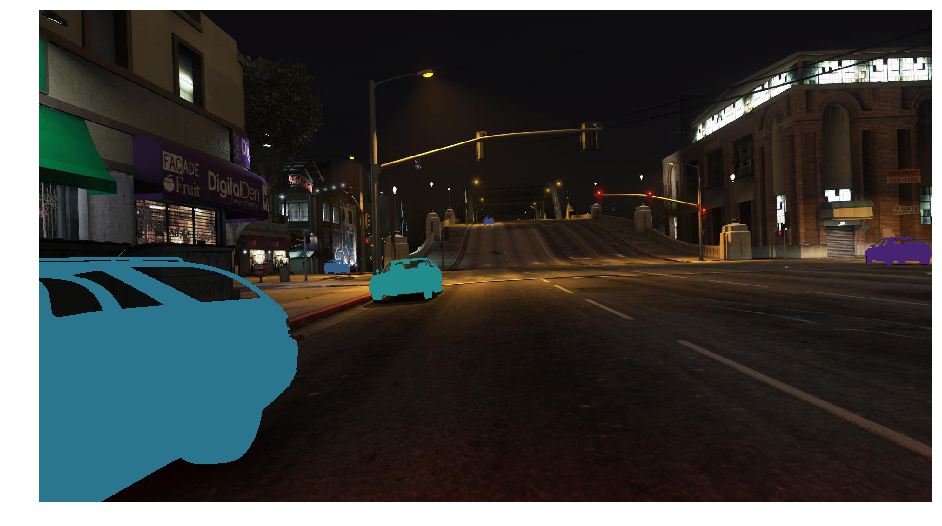
\includegraphics[width=12cm]{obrazky/pixelwise-night}
\par\end{centering}
\caption{pixel-wise annotation of cars}
\end{figure}

\begin{figure}
\begin{centering}
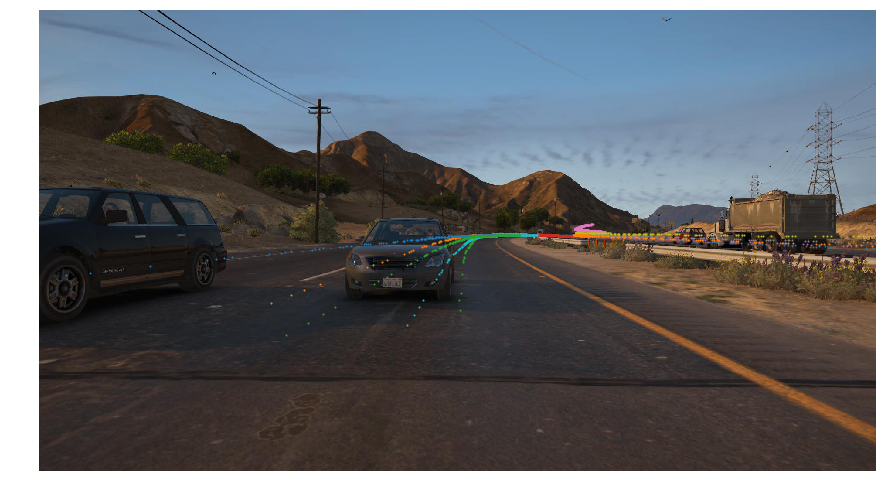
\includegraphics[width=12cm]{obrazky/trajectories-day}
\par\end{centering}
\caption{individual car trajectories}
\end{figure}

\begin{figure}
\begin{centering}
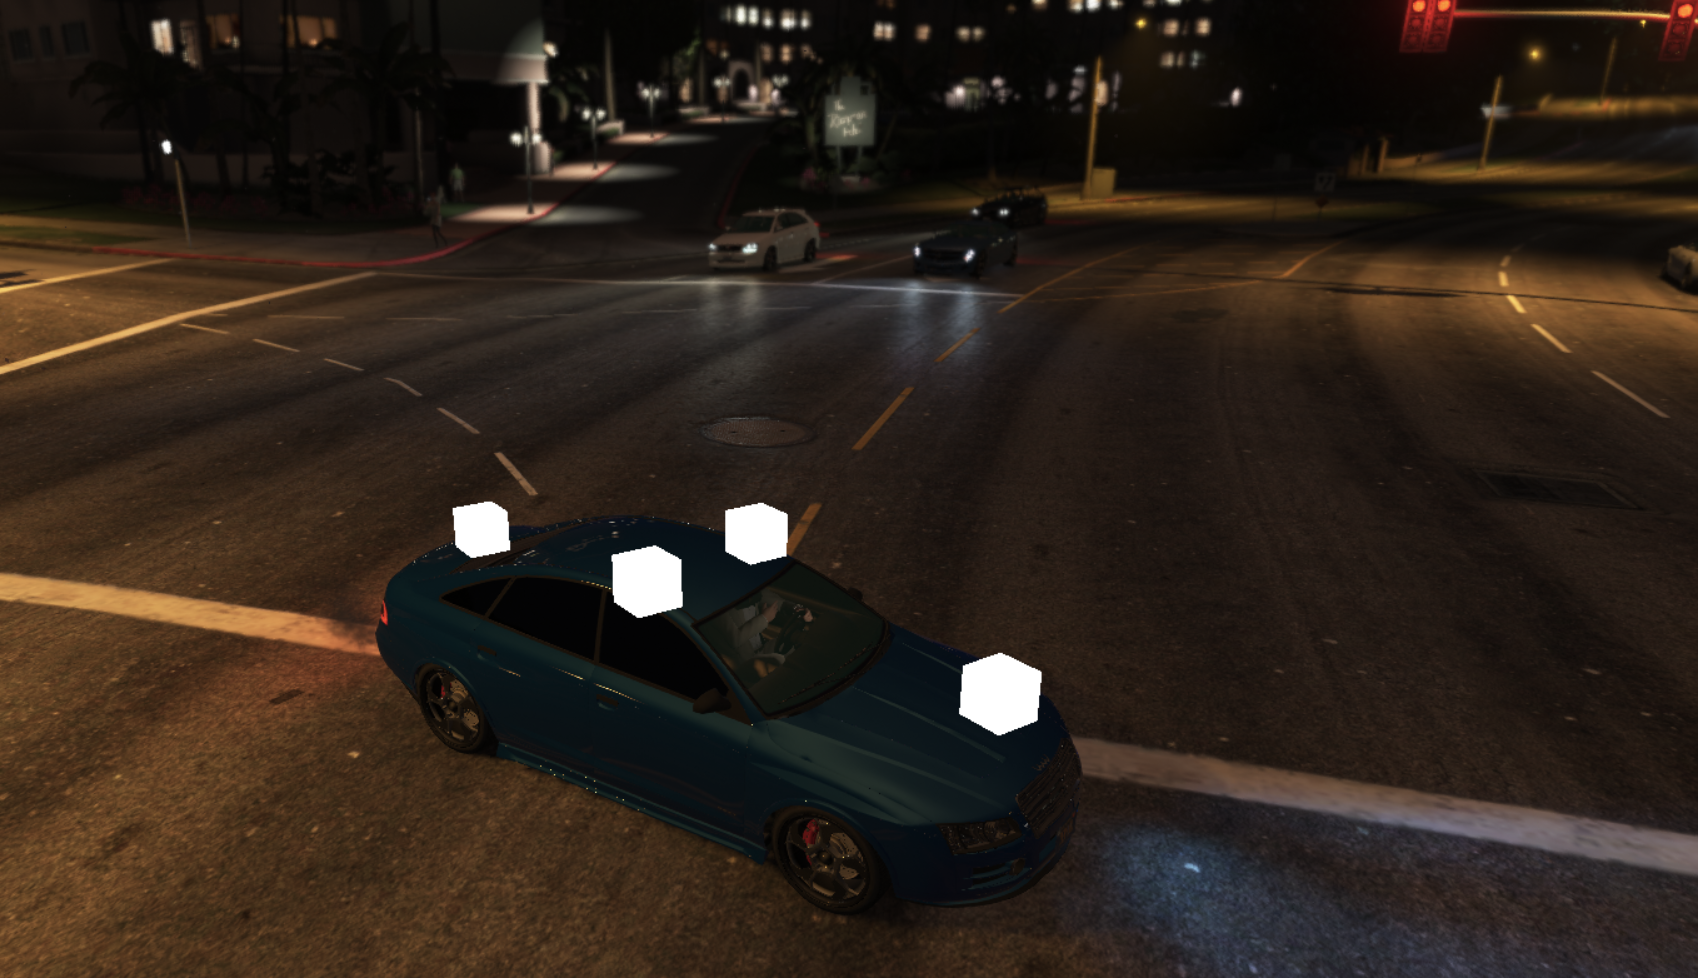
\includegraphics[width=12cm]{obrazky/dataset-2-cameras}
\par\end{centering}
\caption{\label{fig:Camera-positions-for}Camera positions for second dataset}

\end{figure}


\chapter{3D map estimation}

When thinking of 3D map estimation, we can utilize the similarity
between 3D map estimation and the depth estimation, because in depth
estimation, we predict the distance of nearest object pixel-wise,
and in 3D map estimation, we have multiple depth levels per pixel
and estimate occupancy per each depth level. The neural network output
is cuboid with size of $X\times Y\times Z$ neurons, hence it is useful
to represent 3D map of a cuboid as a voxel map with X width levels,
Y height levels and Z depth levels. Then we can estimate occupancy
per voxel, in other words, per each neuron output. Thus we can represent
both depth and 3D map estimation as similar instances, depth estimation
being multi-class occupancy classification per pixel where classes
are depth bins, and 3D map estimation being occupancy classification
per voxel, where we predict occupancy for each voxel.

\section{TensorFlow}

In the neural networks research, one of the important factors is the
ability to easily and efficiently prototype new architecture and train
neural network. TensorFlow \cite{tensorflow2015-whitepaper} is a
framework for developing and training neural networks, developed by
Google Inc. It is based on declarative programming and the API provides
a way to describe the computational graph. This graph is can be then
queried for value of any node in the graph given specific input. Other
advantage of TensorFlow is almost seeming-less transition between
running the calculation graph on CPU and on GPU which allows to users
to describe abstract mathematical operations without the need of low-level
optimizations of calculations on CUDA, everything is taken care of
by TensorFlow. As a powerful tool for introspections of neural network
training, TensorBoard was developed as a visualization utility for
TensorFlow. During the training, certain parameters can be logged
periodically and then visualized in TensorBoard, enabling visualization
of cost function, metrics, input and output images, or weight histograms
in time, which leads to more intuitive understanding of issues during
solving problems with neural networks training. 

\section{Depth estimation}

As a task preceding the 3D map estimation, I firstly trained neural
network for depth estimation. There are many datasets for depth estimation,
but most of them are either indoor with relatively precise ground
truth depth or outdoor with sparse depth labels, like in KITTI dataset
\cite{kitti}, or they are in relatively low resolution and loss accuracy
in higher distance \cite{make3d-dataset}, which is natural for real-world
depth measurement. For training, I use Closed VirtualScapes dataset,
synthetic dataset gathered from GTA V, described in section \ref{sec:Datasets-proposal}. 

This dataset is already in the form of corresponding RGB and depth
images, but the depth is in the NDC space so it must first be pixel-wise
transformed into the camera view space where the depth is in meters.
We might train network directly in the NDC space, but the depth reconstruction
learned would be deformed. The NDC space is not linearly mapped into
the camera view space, in fact, it is mapped hyperbolically, according
to the visualization pipeline \cite{real-time-rendering}. After obtaining
the depth in meters, I performed depth binning to obtain the depth
representation for the classification task. Since these data are outdoor,
the depth varies from 1 meter to 10km, which is the camera far clip
and nothing after 10km is rendered. Which is still much bigger depth
range than in real world datasets. Depth estimation of very distant
objects is harder than for close ones, mainly because their relative
size on the image is lot smaller, but also small difference in image
can mean big depth difference in meters. And in most of applications,
we are interested only in relatively near objects depth estimation.
This is why the depth range to 50 meters has been used for binning
into 100 depth levels, and one additional depth level was used as
the ``another'' class, depth out of the range, so network would
still classify far away pixels as some bin and wouldn't try to assign
them some nearer depth level. This is why there are 101 channels in
the network output. Due to this setup, ground truth depth which is
used as the correct label during training, has all pixels more distant
than 50 meters belong to the same depth class. This is important for
visual evaluation of predicted depths.

In convention in neural networks for image processing each layer has
usually 4 dimensions. Those dimensions have semantics (batch size,
image height, image width, number of channels). The batch size is
usually omitted in most of notations because it is constant in all
network. Other dimensions change its size in individual layers.

The basic architecture for depth estimation is based on Li et al.
\cite{depth-estimation-hierarchical-fusion-soft-weighting}, but there
are modifications. The whole network can be seen in figure \ref{fig:Depth-estimation-neural}.
The input is $320\times240$ RGB image. Bigger images are resized
to this size. The overall architecture and individual parameters should
be visible in the figure. In each box, the first row is the type of
neural network layer, other rows specify either its parameters, or
next layer. Conv means convolutional layer, next row after it specifies
its parameters, namely kernel, size of last dimension (also sometimes
called number of channels), stride, and activation function. For instance,
in the second box, second row, ``7x7, 64, 2, relu'' means 7x7 kernel,
last 64 output channels, stride 2 and Rectified Linear Unit activation
function. When no activation function is specified, there is no activation
function and convolutional layer output is directly input to the consecutive
layer. Most of the network consists of two types of block. Resize
blocks and non-resize blocks. The naming comes from the property of
convolutional layers, specifically the stride parameter. When the
stride is 1, width and height dimensions remain unchanged, but when
the stride is higher, the width and height are resized. These blocks
are the main building blocks of the ResNet network \cite{resnet}
and we can see the layers for residual mapping in non-resize blocks.
Non-resize blocks are stacked onto each other multiple times, which
is denoted in the figure, specifically non-resize blocks are repeated
2, 7, 35 and 2 times, respectively. As depicted in the figure, output
of all blocks from the second resize block onwards are then concatenated
together in the channel dimensions, which allows utilization of low-level,
mid-level and high-level feature is the last layers of the network.
The input layer is denoted by the green background, output layer by
blue background, and orange and yellow backgrounds represent layers
with dilated convolution. Orange background is used for blocks whose
convolution layers uses dilution in rate 2, which means neighbouring
neurons in the convolution mask have distance=2 from its neighbours,
every second neuron is omitted in each direction. The similar property
holds for blocks with yellow background, where the dilated convolution
has rate 4, which means neighbouring neurons in the convolution mask
are 4 neurons distant from each other in the previous layer.

\begin{figure}
\begin{centering}
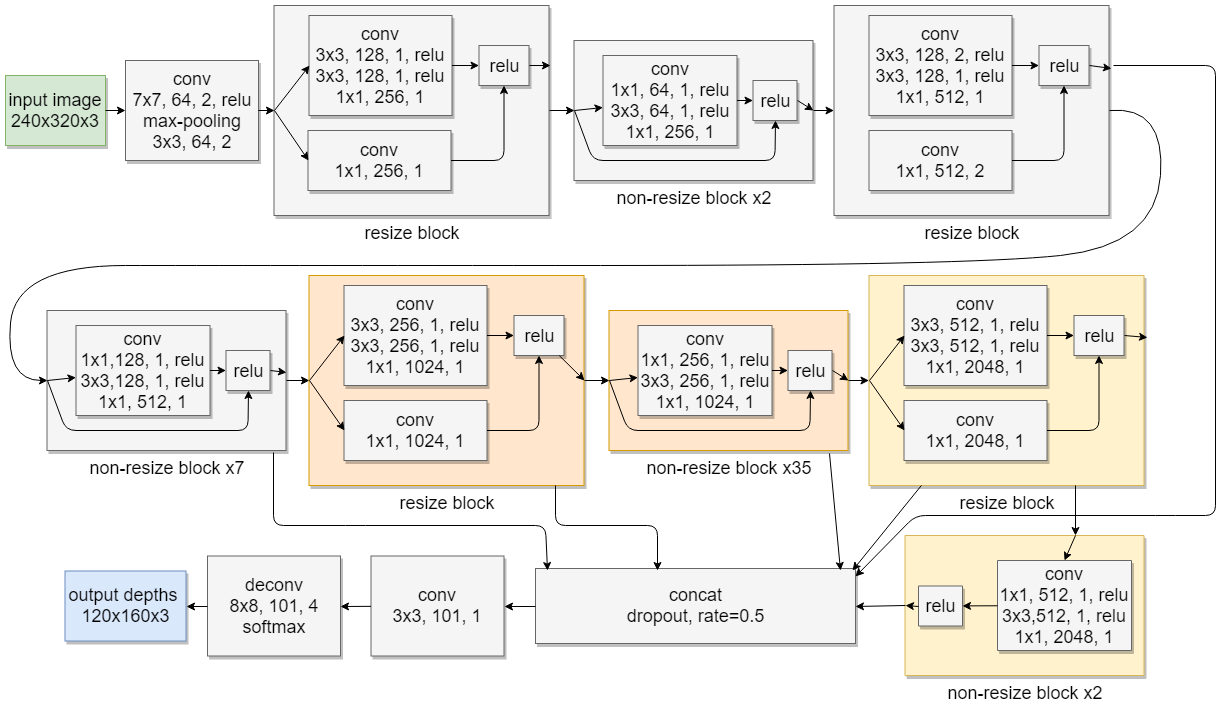
\includegraphics[width=14cm]{obrazky/my-master-network-depth}
\par\end{centering}
\caption{\label{fig:Depth-estimation-neural}Depth estimation neural network}
\end{figure}

Layers of network which have same architecture as ResNet-152 have
been initialized by trained ResNet network. For remaining parameters
the following holds. Weights of neuron inputs have been initialized
by Xavier initialization from normal distribution, and biases have
been initialized to the constant value 0.1. After each layer, the
batch normalization has been used, with $\epsilon=10^{-3}$ and decay$=0.9997$.
During the training, the cost is optimized, but it is hard to compare
results when different cost is tried only based on visual perception,
which is why other metrics are being used for evaluation the accuracy
of trained network. For depth estimation, following metrics are reported.
Accuracy under threshold, mean relative error, root mean squared error,
mean squared log error, and average $\log_{10}$ error. All of them
are calculated pixel-wise.They are formally defined as follows. 
\begin{enumerate}
\item Accuracy under threshold $aut\left(\tau\right)=\frac{1}{K}\stackrel[i=1]{K}{\sum}1\left\{ \max\left(\frac{d_{i}^{*}}{d_{i}},\frac{d_{i}}{d_{i}^{*}}\right)<\tau\right\} $
\item Mean relative error $rel=\frac{1}{K}\stackrel[i=1]{K}{\sum}\frac{|d_{i}^{*}-d_{i}|}{d_{i}^{*}}$
\item Root mean squared error $rms=\sqrt{\frac{1}{K}\stackrel[i=1]{K}{\sum}\left(d_{i}^{*}-d_{i}\right)^{2}}$
\item Root mean squared log error $rmslog=\sqrt{\frac{1}{K}\stackrel[i=1]{K}{\sum}\left(\log_{10}\left(d_{i}^{*}\right)-\log_{10}\left(d_{i}\right)\right)^{2}}$
\item Average $\log_{10}$ error $logerr=\frac{1}{K}\stackrel[i=1]{K}{\sum}|\log_{10}\left(d_{i}^{*}\right)-\log_{10}\left(d_{i}\right)|$
\end{enumerate}
where $d_{i}$ is predicted depth on $i$-th pixel, $d_{i}^{*}$ is
the ground truth depth on $i$-th pixel, $K$ is the total number
of pixels per sample, and $\tau$ is the threshold for accuracy under
threshold. The most frequent value is $\tau=1.25$, and this is also
used during evaluations of this thesis. Other frequently used values
are $\tau=1.25^{2}$ and $\tau=1.25^{3}$. 

\section{3D map estimation}

The 3D map estimation from single RGB image is an abstract task and
has many possible representations. In many tasks, voxel-map has proven
to be good representation of the 3D space. Voxel (volumetric pixel)
is the smallest distinguishable unit in 3D space, it is 3D analogy
of 2D pixel. In this scenario, each voxel has one of three states:
free, occupied and unknown. The size of voxel is not generally set
and is being chosen to fit particular task. Too big voxel size causes
high loss of information, and too small voxel size leads to high amount
of voxels, more complicated manipulation with the resulting voxelmap
and higher size when persisting the voxelmap. 

Image which is used as an input for 3D map estimation is representing
only a frustum in 3D map and does not contain information about space
outside of this frustum. Because of this fact, setup in this thesis
focuses only on reconstruction of 3D space inside the frustum viewed
by the camera taking the image. Output of the neural network is $X\times Y\times Z$
cuboid, which will be mapped to the frustum so output of each neuron
represents point in the frustum. Mapping between the the cuboid and
frustum is contained in the projection matrix \ref{subsec:Camera-to-NDC}
which is used for the training dataset creation and for reconstruction
of pointcloud from neural network output during prediction. With this
setup, the model is predicting occupancy of points sampled from the
frustum. In my setup, the frustum will be up to 25m from camera.

\subsection{Training dataset construction from depth images}

The synthetic dataset created from GTA V contains depth images and
camera parameters, so there is need to reconstruct the 3D map and
sample it to create the training dataset. For 3D map reconstruction,
I gathered data from four cameras with positions relative to the driving
car, as seen in figure X where each white cube represents camera position
\ref{fig:Camera-positions-for-3d}. Totally there are 4 cameras, equally
placed on the circle with 8 meters circumference. This setup will
demonstrate the whole process of building 3D frustum map from 4 cameras.

\begin{figure}
\begin{centering}
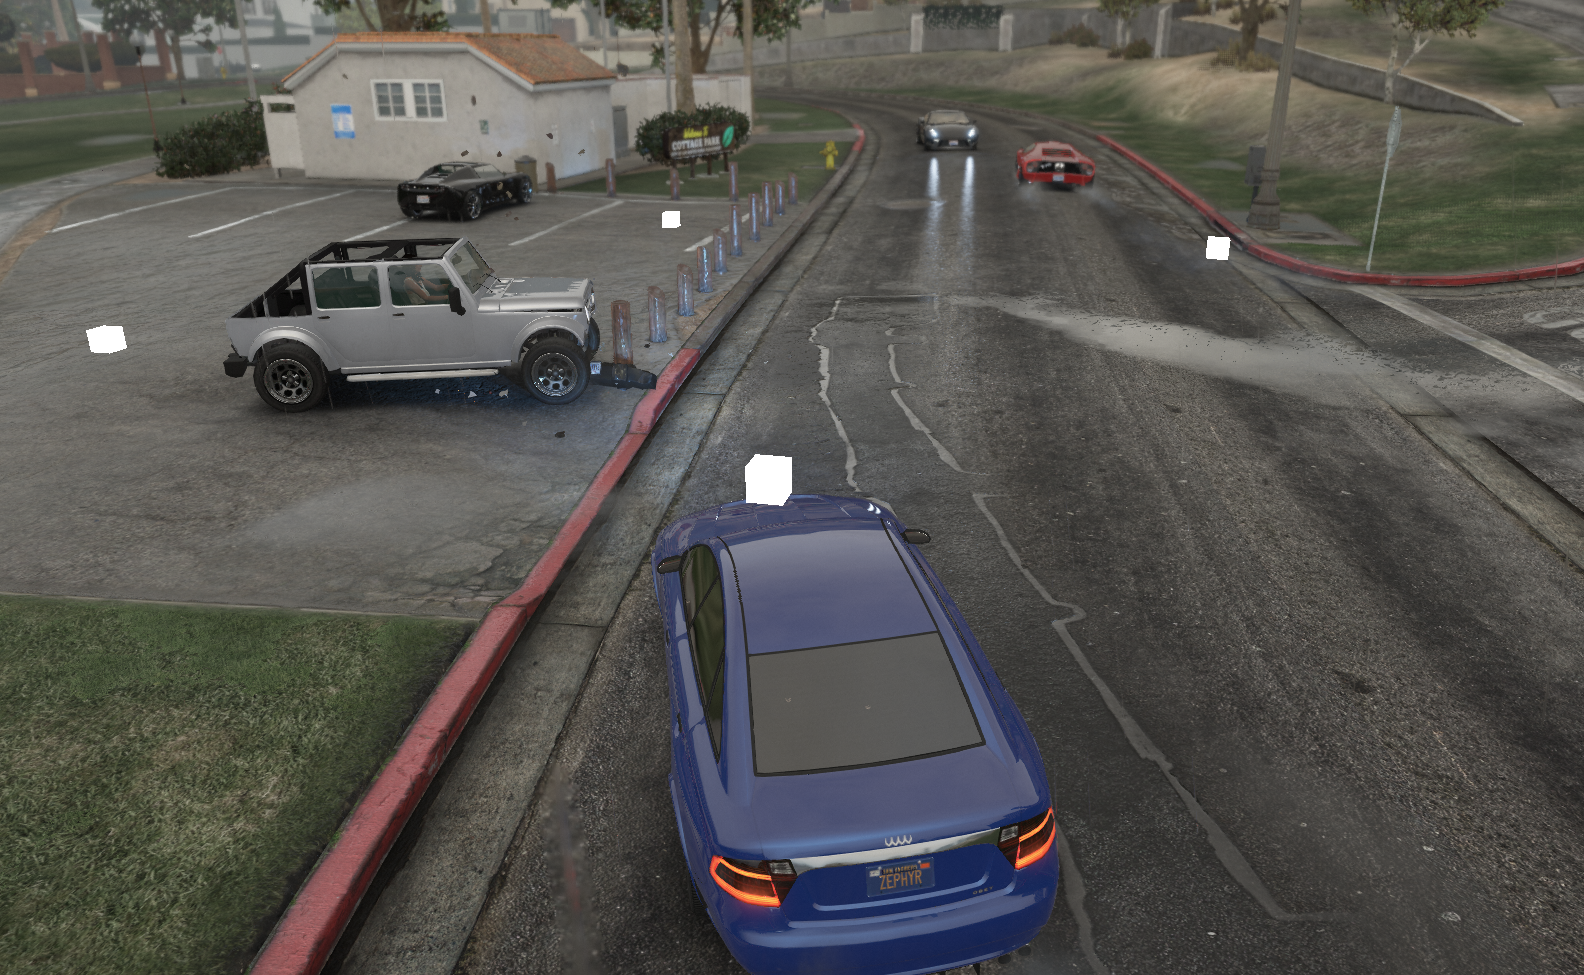
\includegraphics[width=12cm]{obrazky/dataset-1-cameras}
\par\end{centering}
\caption{\label{fig:Camera-positions-for-3d}Camera positions for 3d reconstruction}
\end{figure}

\begin{figure}
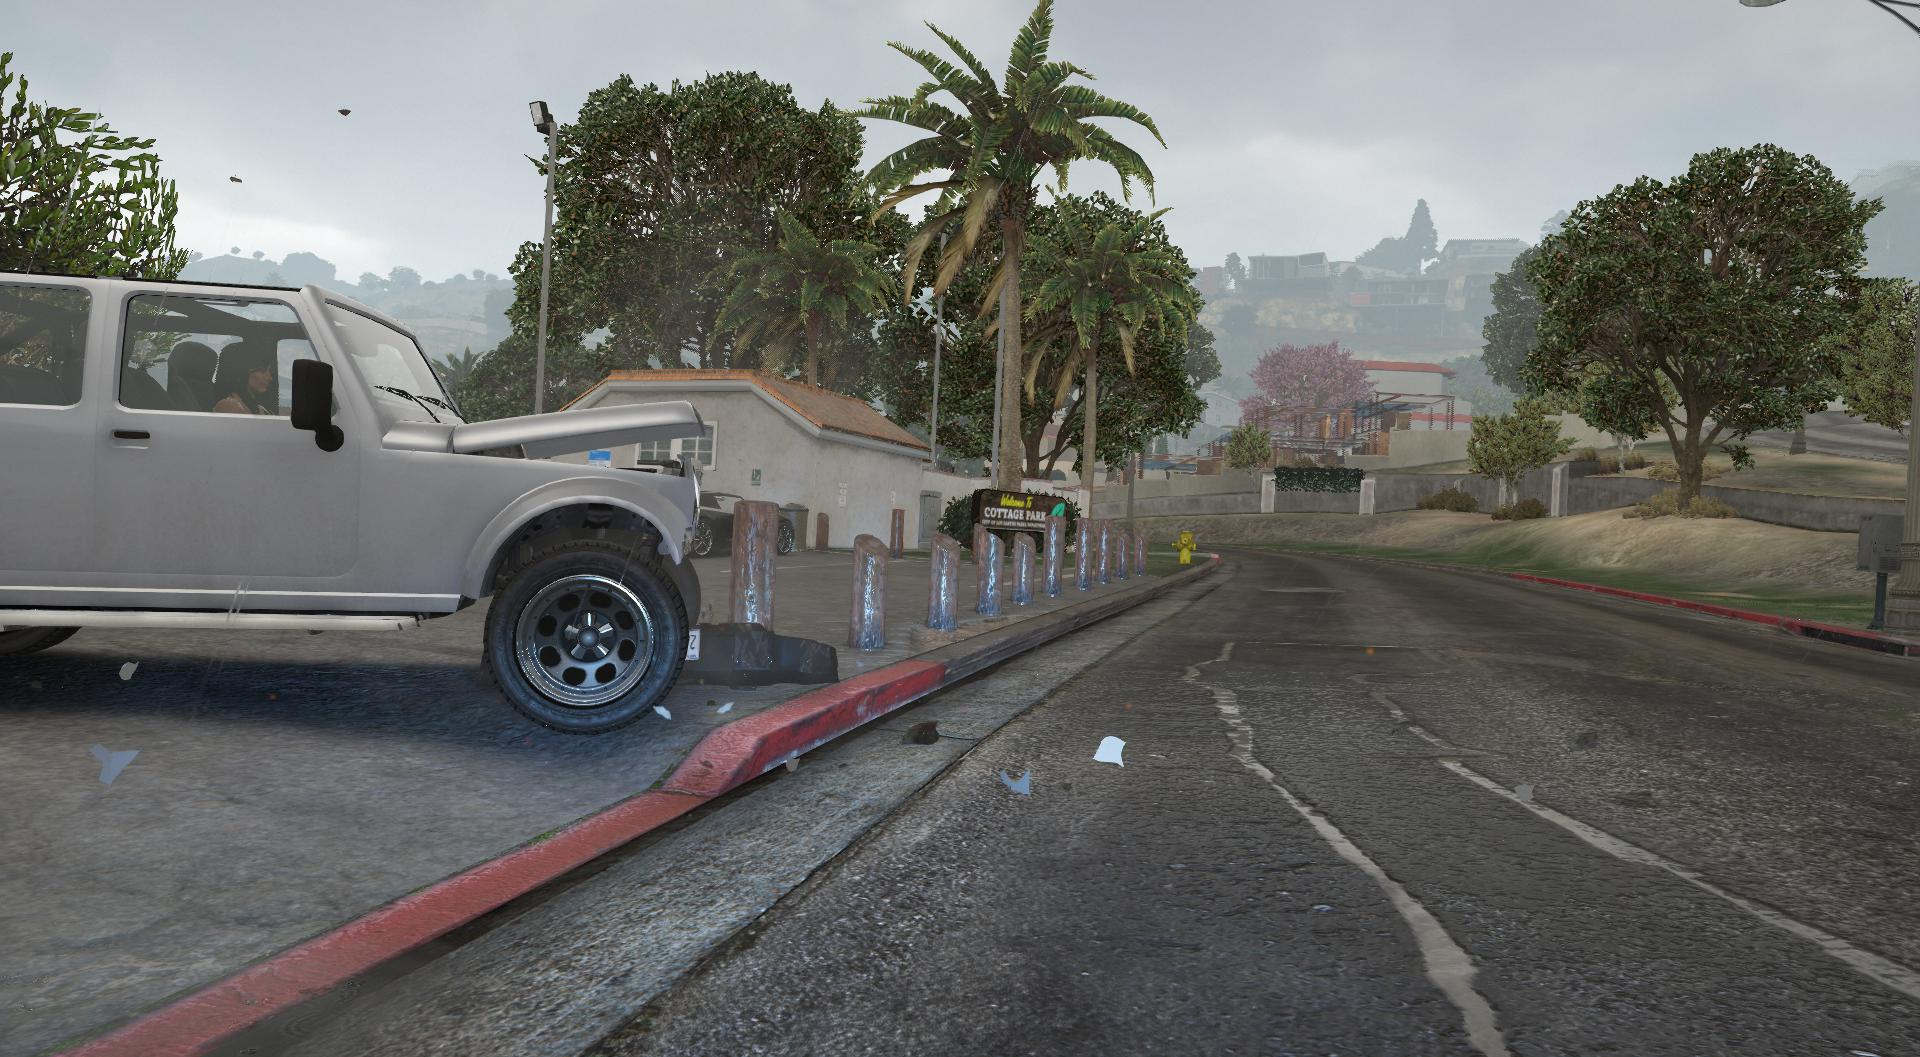
\includegraphics[width=7cm]{obrazky/2018-05-08--14-15-35--576}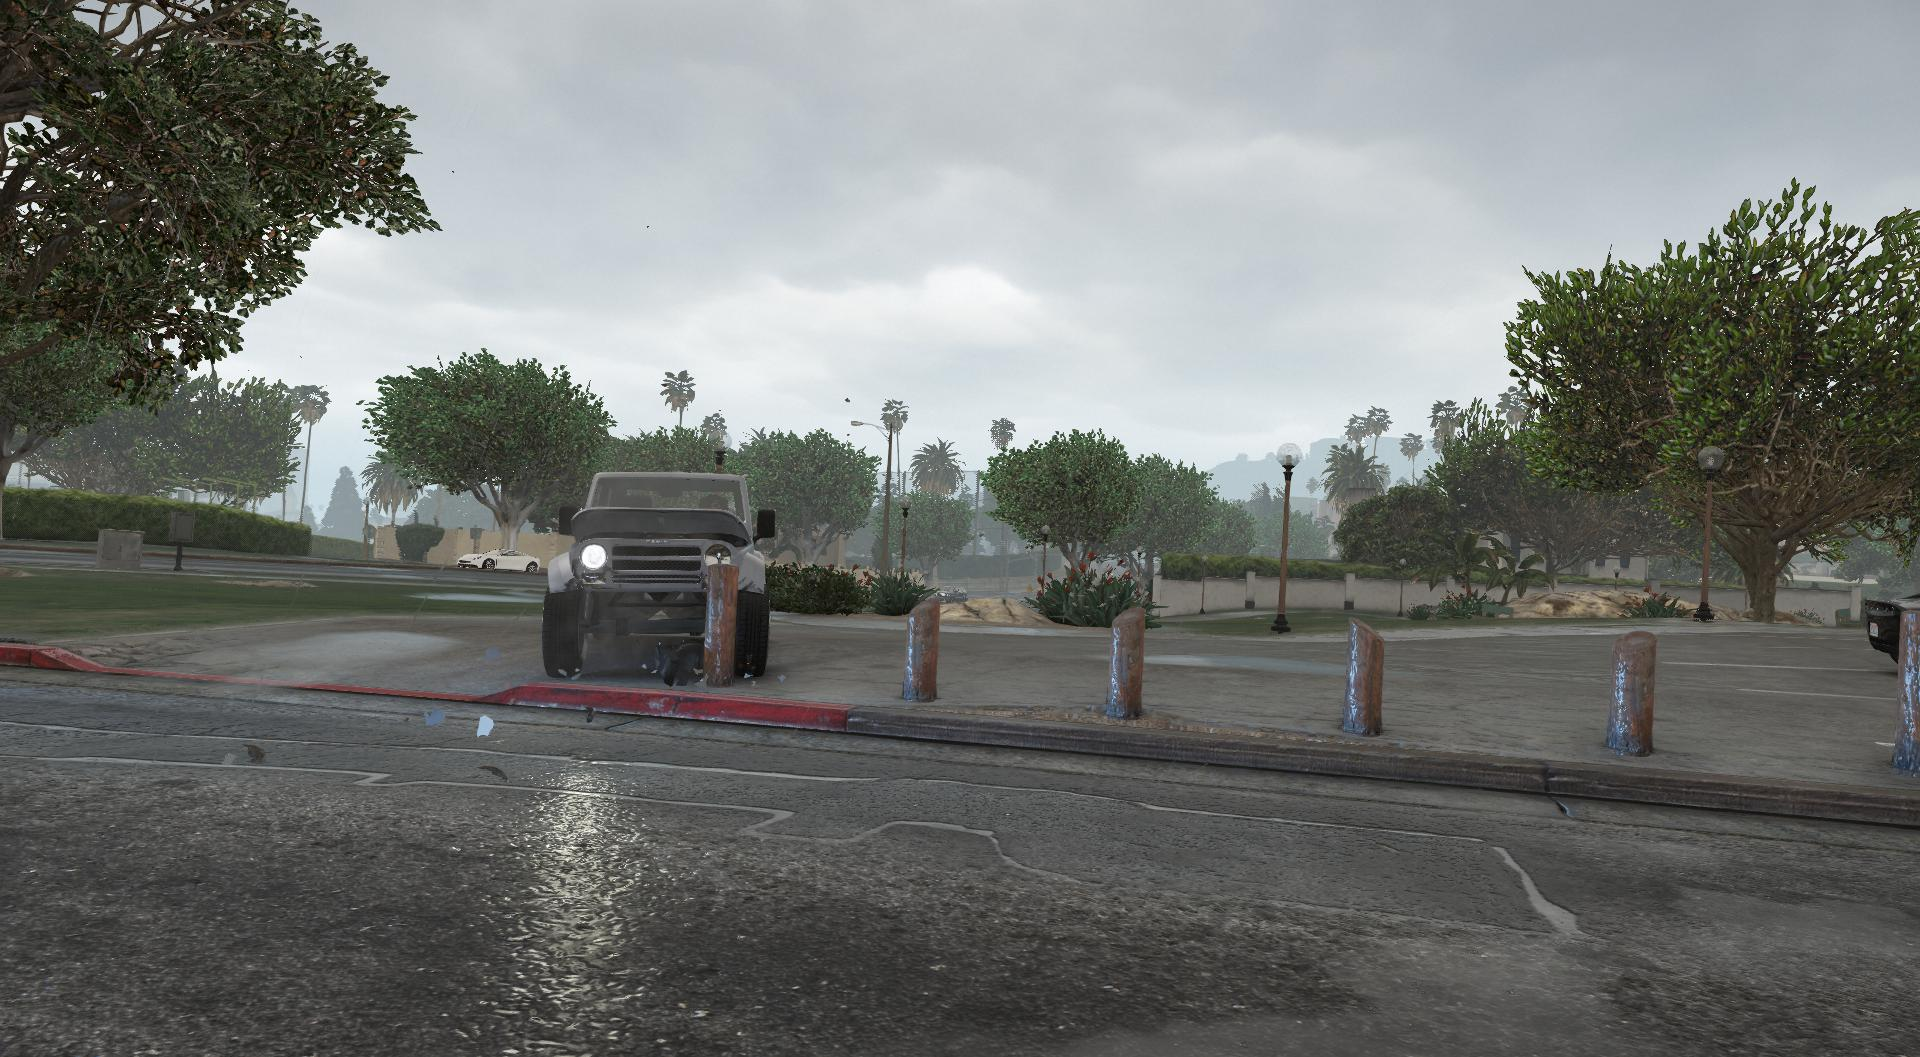
\includegraphics[width=7cm]{obrazky/2018-05-08--14-15-35--972}

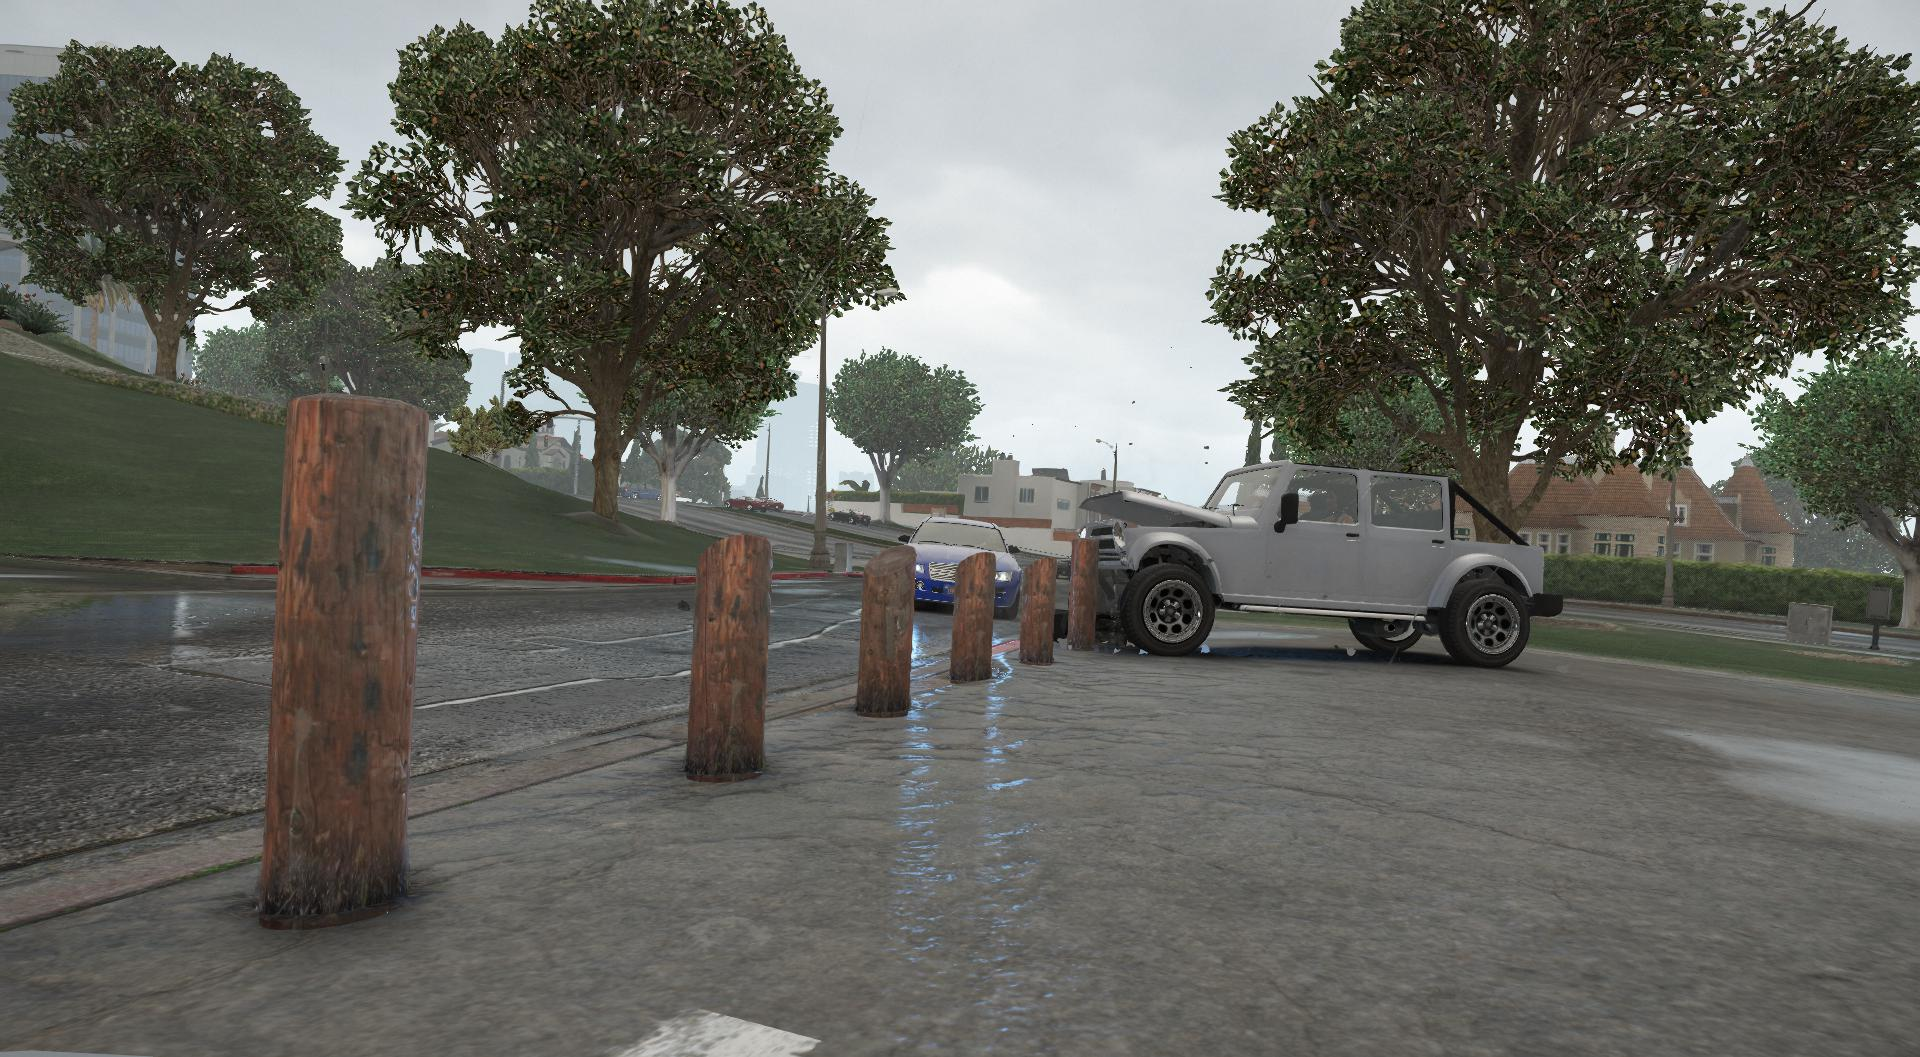
\includegraphics[width=7cm]{obrazky/2018-05-08--14-15-36--349}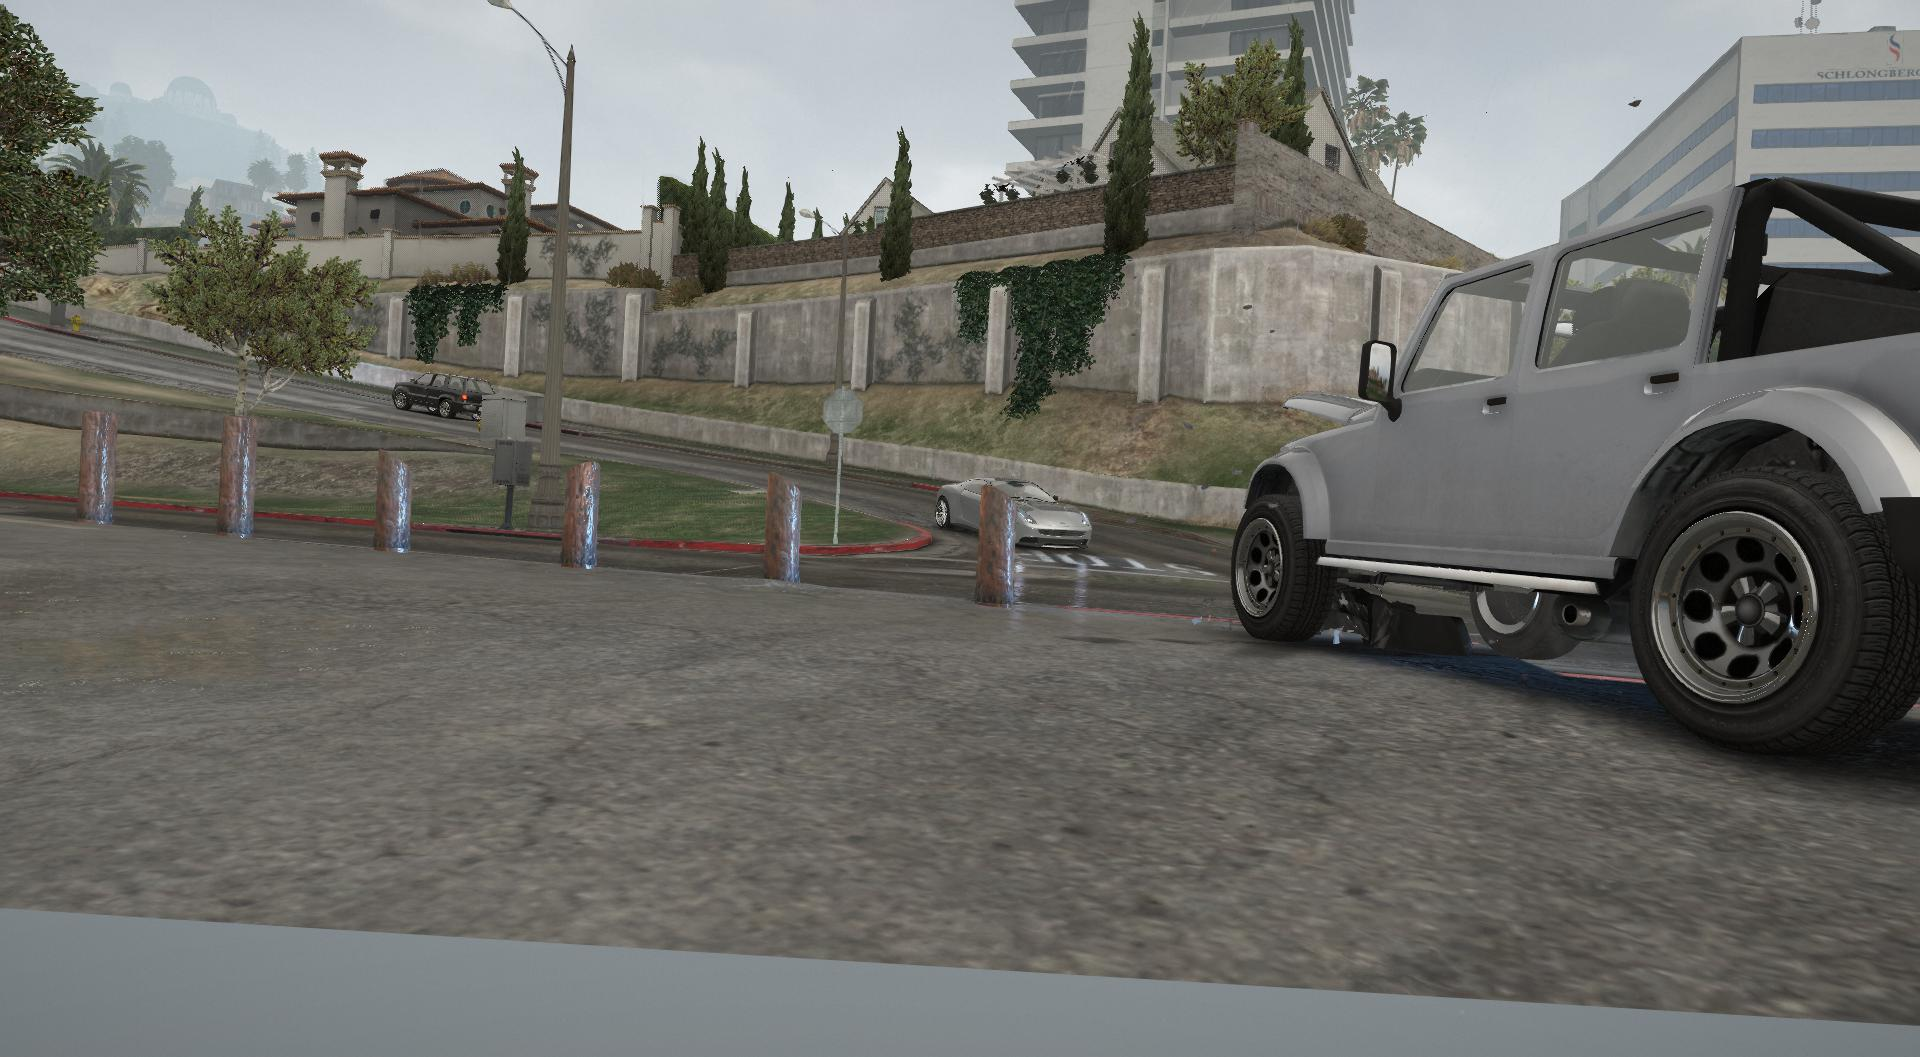
\includegraphics[width=7cm]{obrazky/2018-05-08--14-15-36--728}\caption{\label{fig:extracted-RGB-images}extracted RGB images from 4 cameras}

\end{figure}

\begin{figure}
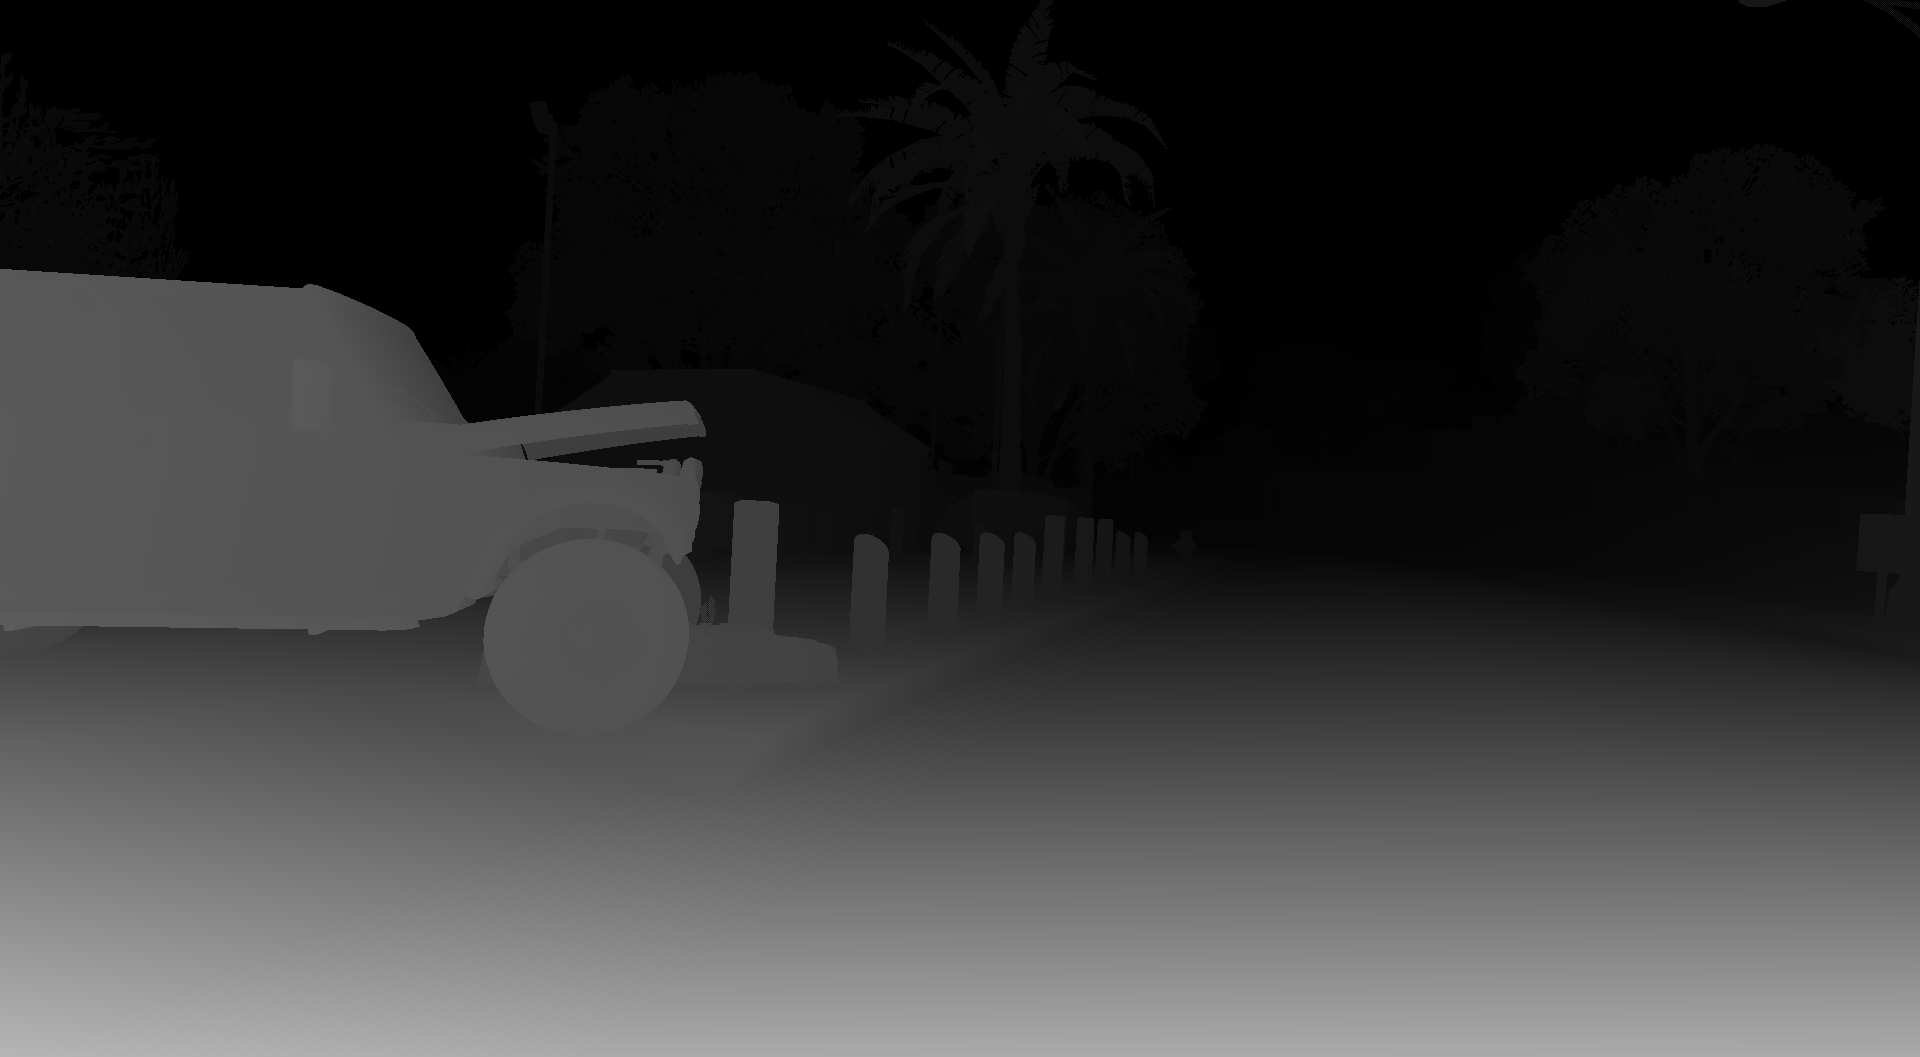
\includegraphics[width=7cm]{obrazky/2018-05-08--14-15-35--576-depth}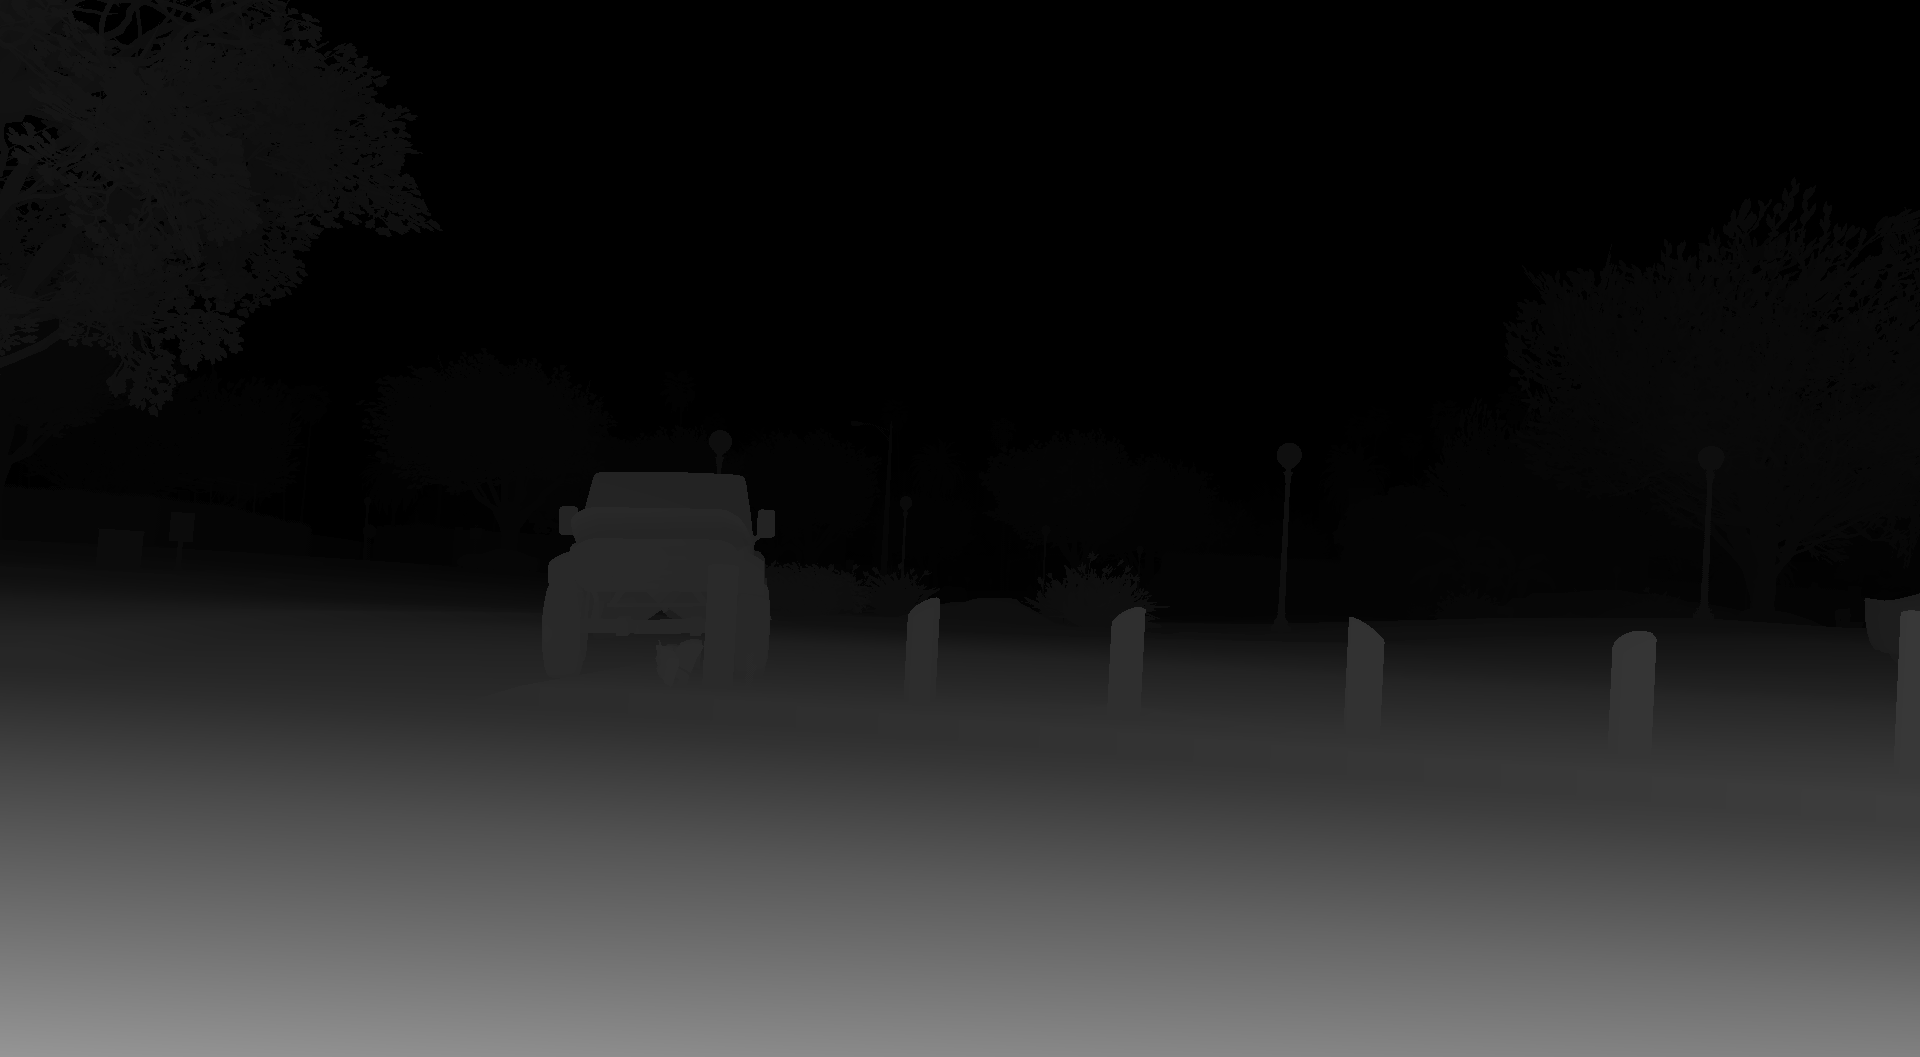
\includegraphics[width=7cm]{obrazky/2018-05-08--14-15-35--972-depth}

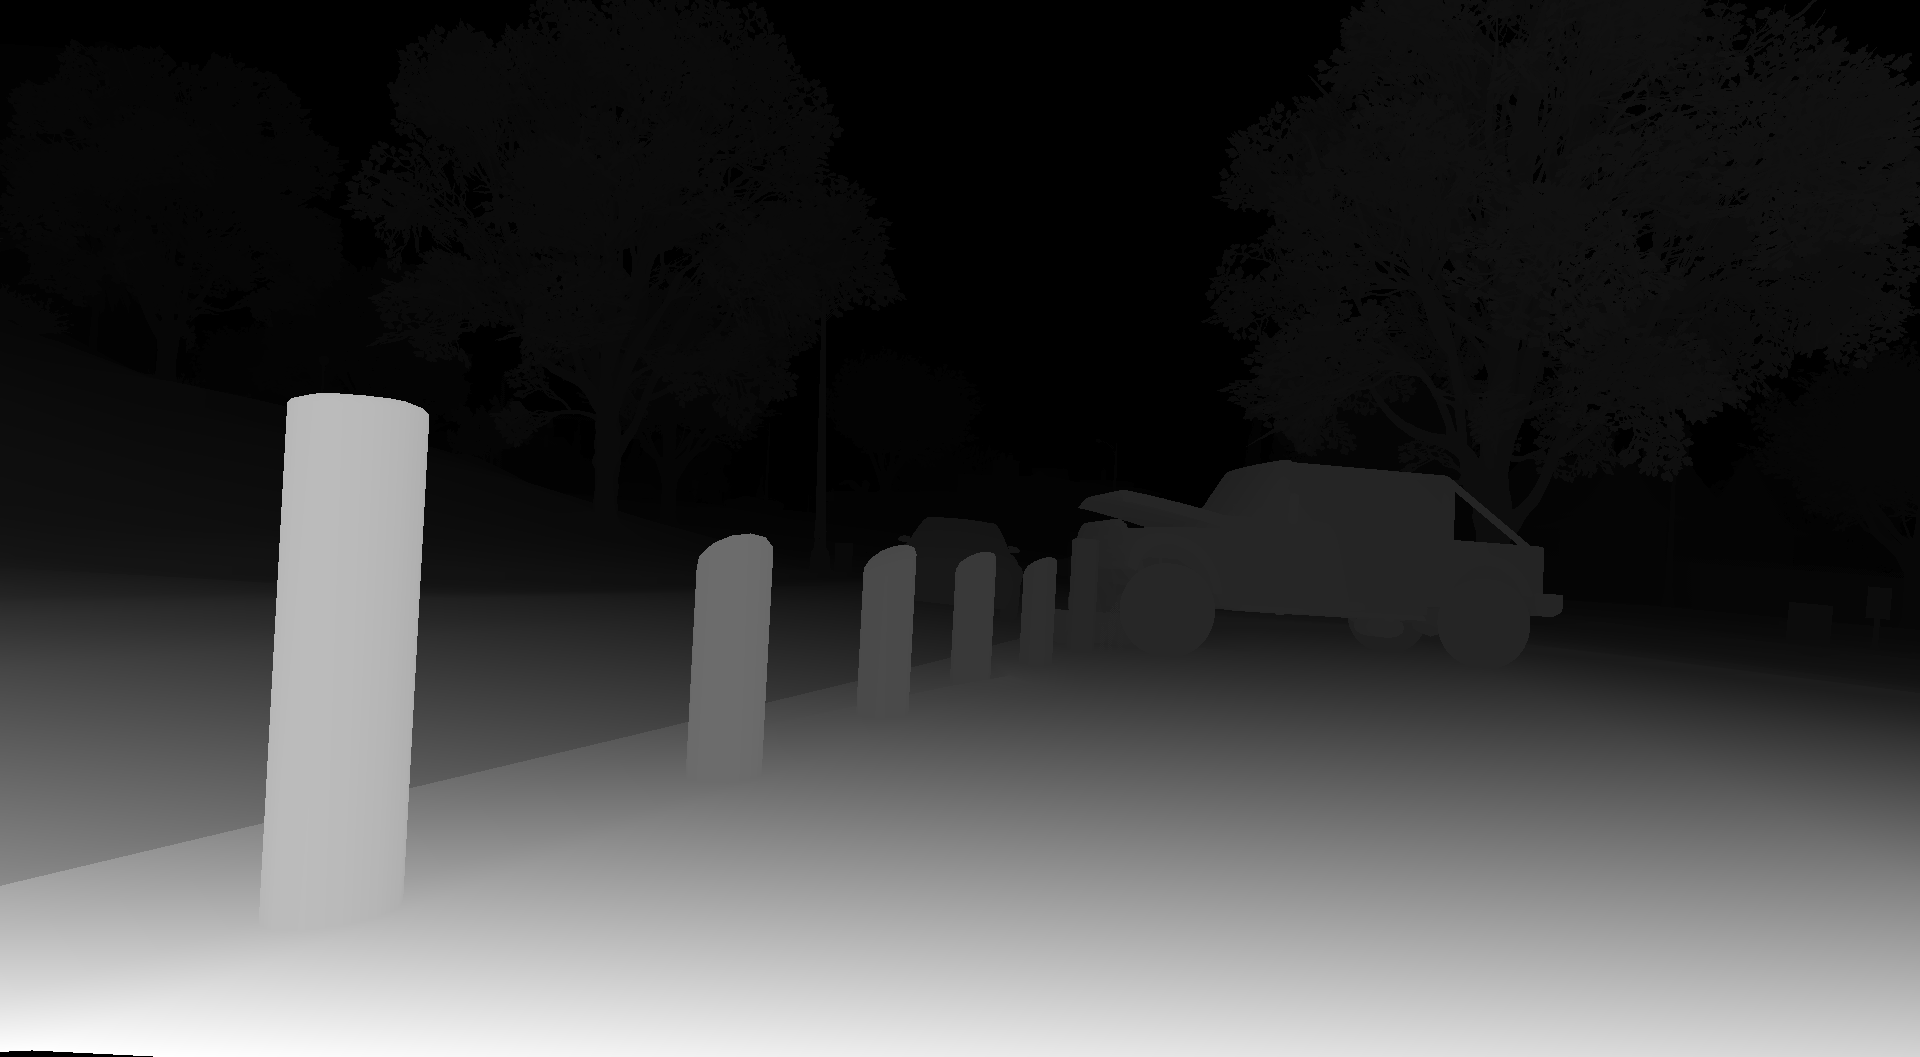
\includegraphics[width=7cm]{obrazky/2018-05-08--14-15-36--349-depth}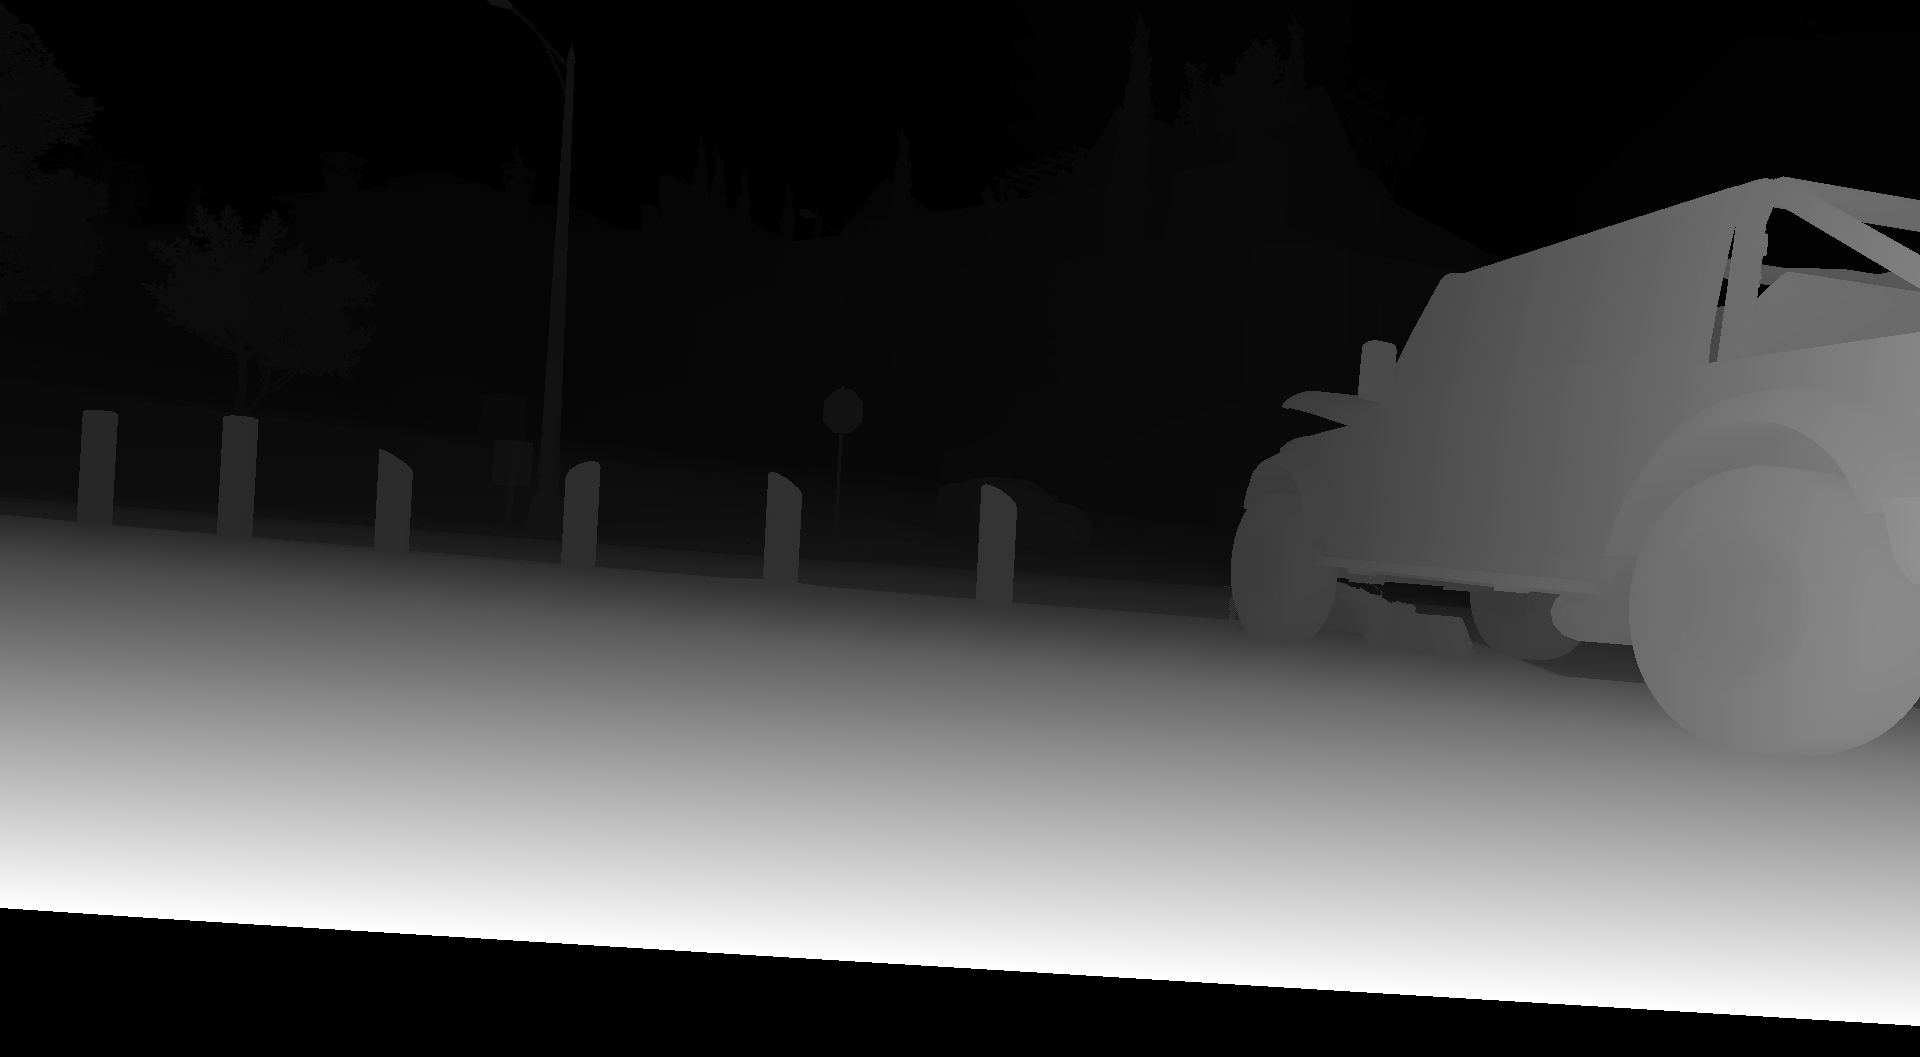
\includegraphics[width=7cm]{obrazky/2018-05-08--14-15-36--728-depth}\caption{\label{fig:extracted-depth-images}extracted depth images from 4 cameras}
\end{figure}
From these 4 cameras, I gathered 4 RGB and depth images, shown in
figures \ref{fig:extracted-RGB-images} and \ref{fig:extracted-depth-images}.
I also gathered camera parameters, namely position, rotation, near
clip, and field of view. With these parameters, depth images can be
easily transformed into the pointcloud in world coordinate system.
Let us have $\boldsymbol{I}^{1}$depth image from the 1st camera with
with width $W$ and height $H$ pixels. Since depth image contains
value in NDC space then, $\boldsymbol{I}^{1}=\left(d_{i,j}\right)\in\left[0,1\right]^{W\times H}$
holds, where $d_{i,j}$ is value of pixel with coordinates $\left[i,j\right]$.
For every pixel, we know its depth value and coordinates in the pixel
space, thus we can describe it as a point in NDC space
\[
\boldsymbol{x}_{i,j}^{NDC}=\begin{bmatrix}x^{NDC}\\
y^{NDC}\\
z^{NDC}\\
1
\end{bmatrix}=\begin{bmatrix}\frac{2i}{W}-1\\
-\left(\frac{2j}{H}-1\right)\\
d_{i,j}\\
1
\end{bmatrix}
\]
, where the $\boldsymbol{x}_{i,j}^{NDC}$ is pixel$\left[i,j\right]$
transformed into NDC space. The sign change in $y^{NDC}$ is cause
by indexing conventions of images, where lowest pixel height is in
the upper part of image but in NDC space, lowest $y^{NDC}$ value
is in the lower part of image. This holds because $x^{NDC},x^{NDC}\in\left[-1,1\right]$.
With this pixel-wise transformation, we can transform each depth image
$\boldsymbol{I}^{k},k\in1..4$ into pointcloud in NDC $\boldsymbol{P}_{k}^{NDC}$.
By using transformation matrices described in \ref{subsec:World-to-Camera}
and \ref{subsec:Camera-to-NDC} we can transform these pointclouds
from different cameras into the same world coordinate space. Let us
have $P$ matrix from \ref{eq:projection-m} and $V_{k}$ matrix from
\ref{eq:camera-m} denoting the view matrix of $k$-th camera, since
these matrices are regular, we can do the transformation 
\[
\boldsymbol{P}_{k}^{W}=V_{k}^{-1}P^{-1}\boldsymbol{P}_{k}^{NDC}\forall k\in1..4
\]
. Then, all pointclouds are merged into one pointcloud $\boldsymbol{P}^{W}$
of whole scene seen from 4 cameras

\[
\boldsymbol{P}^{W}=\underset{k\in1..4}{\bigcup}\boldsymbol{P}_{k}^{W}
\]
. The resulting pointcloud can be seen in figure \ref{fig:Merged-pointcloud-from}.
In this setup, all images are nearly Full HD, specifically $1920\times1057$.
This leads to pointcloud of size $1920\cdot1057=2029440\thickapprox2M$
points. Most of these points are near camera, in unnecessarily high
density for this application. To decrease the size of pointclouds
and the time to process, them I clustered them into 12cm big voxels
and sampled only 1 point per voxel. This sub-sampling decreases the
pointcloud size from $\sim2M$ points into $\sim80k$ to $\sim120k$
points, which is 4\% to 6\% of original size. This sub-sampling is
performed per depth image so we can easily link each point in pointcloud
with camera it is seen from which is crucial for building occupancy
voxelmap. The far clip is over 10000 \ref{subsec:Reverse-engineering}
and thus the maximum distance from camera is over 10km. For reconstruction
of view frustum to 25m from camera, this is unnecessarily large and
makes further calculation complicated which is why all depth levels
further than 30m were projected into 30m distance before further transformed
into pointcloud. This transformation does not affect the space near
camera but lowers space needed for representation of the pointcloud
during the voxelmap occupancy calculation. Merged pointcloud after
projecting distant points into the 30m distance from their camera
can be seen in figure \ref{fig:Pointcloud-before-and} where I compare
pointclouds before and after aforementioned sub-sampling.

\begin{figure}
\begin{centering}
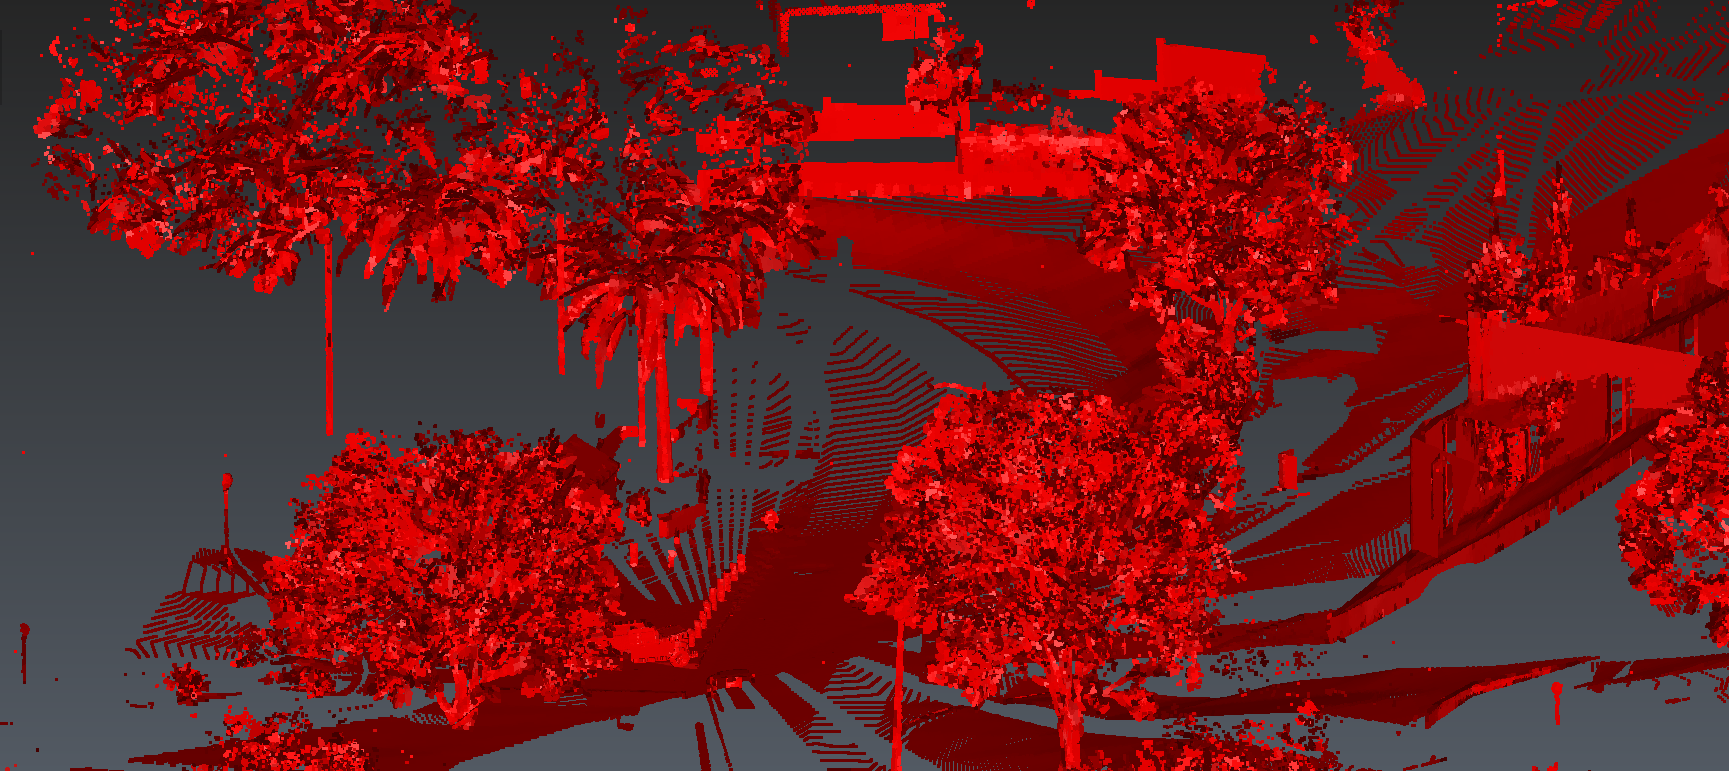
\includegraphics[width=15cm]{obrazky/pcl-orig-1}
\par\end{centering}
\begin{centering}
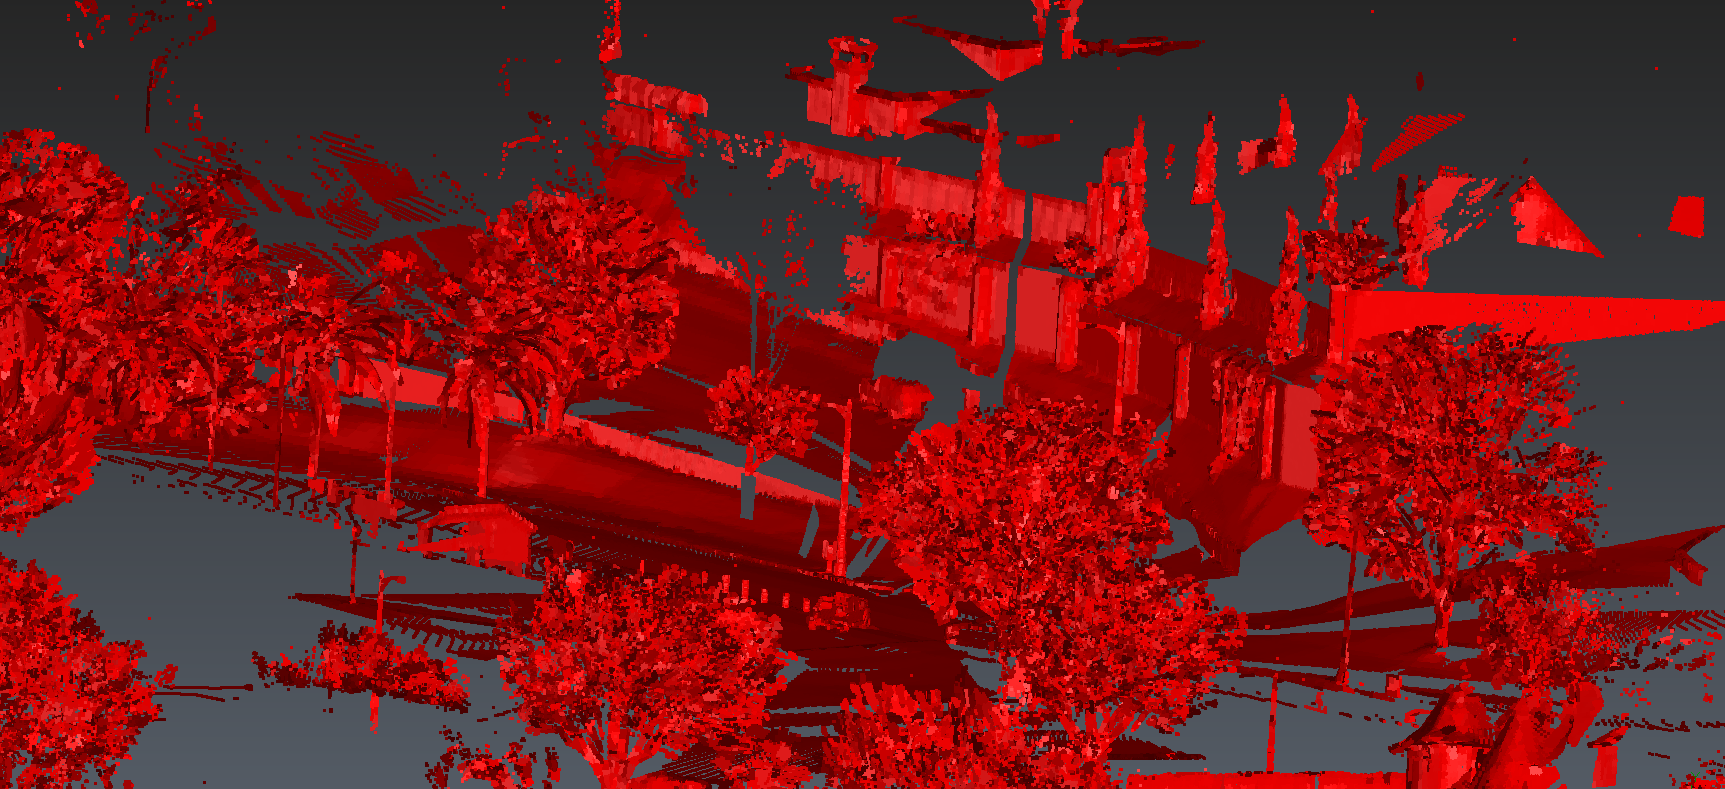
\includegraphics[width=15cm]{obrazky/pcl-orig-2}\caption{\label{fig:Merged-pointcloud-from}Merged pointcloud from all cameras}
\par\end{centering}
\end{figure}

\begin{figure}
\begin{centering}
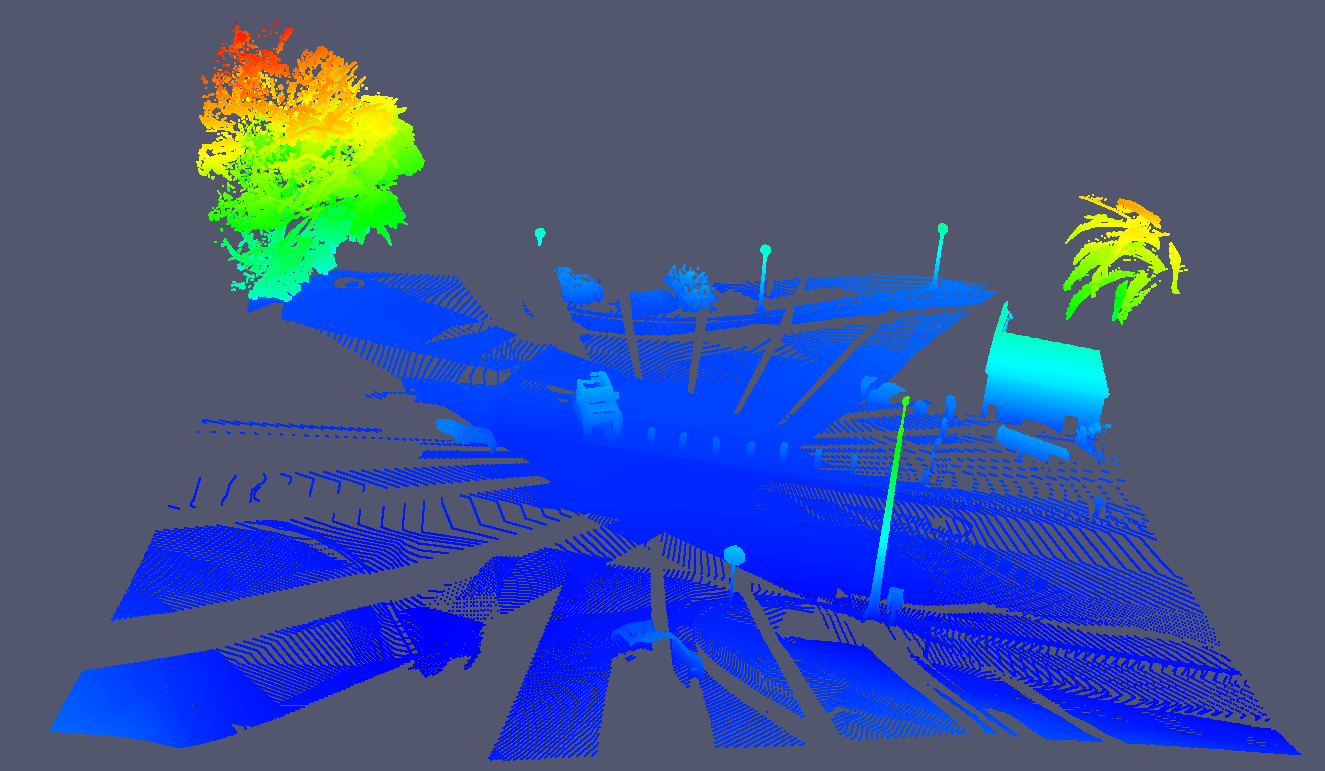
\includegraphics[width=15cm]{obrazky/pcl-full-2}
\par\end{centering}
\begin{centering}
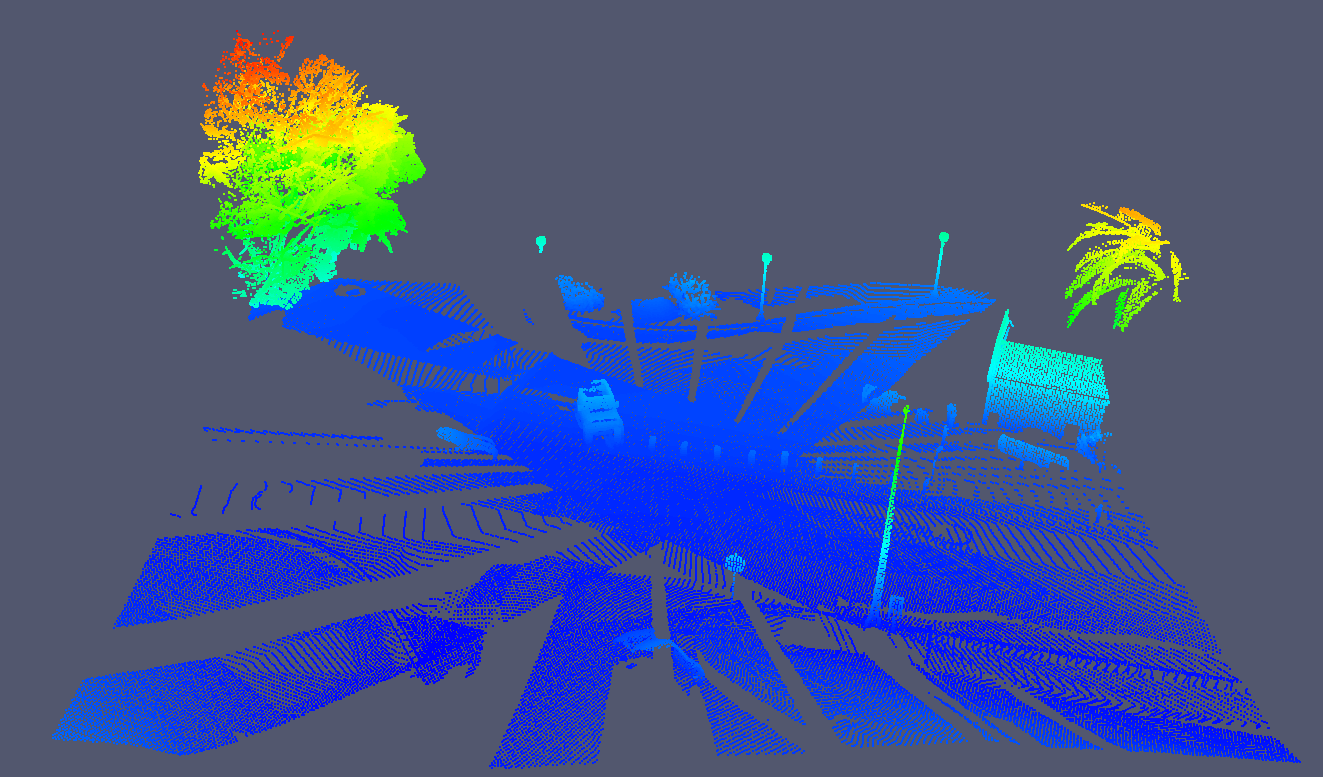
\includegraphics[width=15cm]{obrazky/pcl-sub-2}
\par\end{centering}
\caption{\label{fig:Pointcloud-before-and}Pointcloud before and after sub-sampling}
\end{figure}

After this projection and sub-sampling, I have everything prepared
for building a occupancy voxelmap . Voxels in this setup are 25cm
big, and each voxel is marked either as occupied, free, or unknown.
The resulting occupancy voxelmap is depicted in figure \ref{fig:Occupied-voxels-in}.
The last part of the processing is the sampling of the view frustum
from this occupancy voxelmap. This is directly mapped to the output
of the neural network. Source code with implementation of the processing
pipeline is available at \url{https://github.com/racinmat/GTAVisionExport-postprocessing}.

\begin{figure}
\begin{centering}
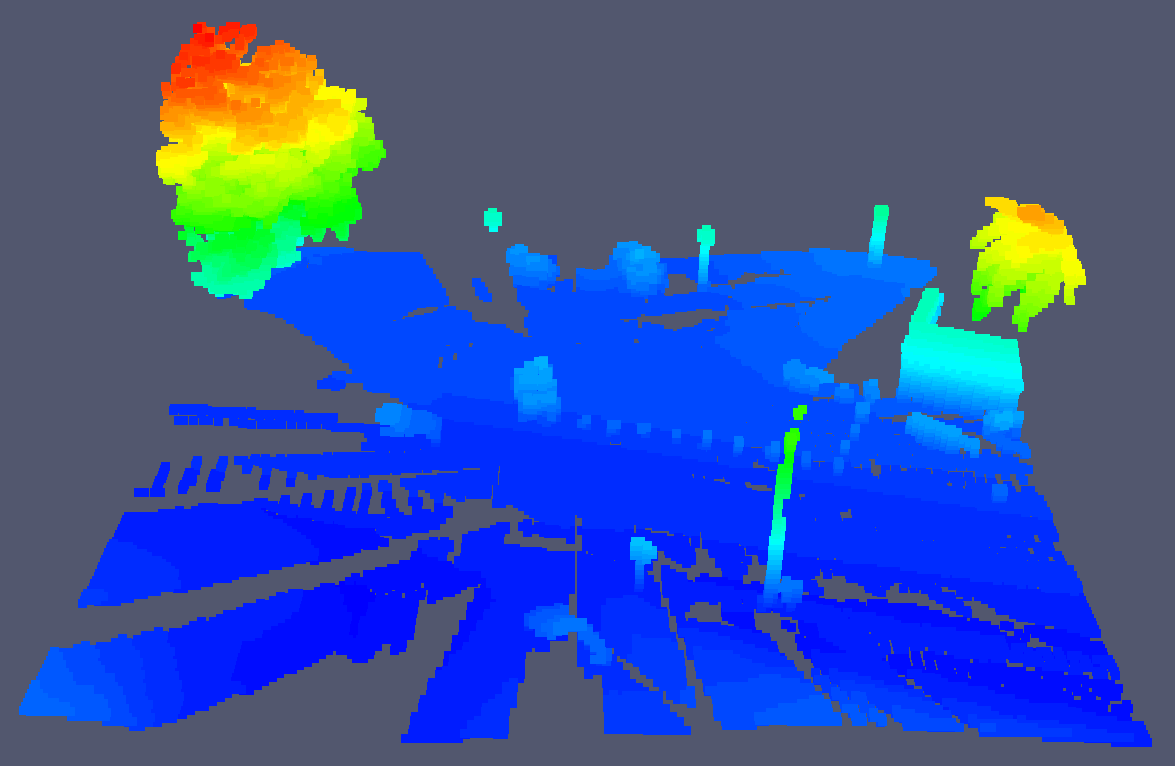
\includegraphics[width=14cm]{obrazky/occupied-pcl-thicc-3}
\par\end{centering}
\caption{\label{fig:Occupied-voxels-in}Occupied voxels in occupancy voxelmap}

\end{figure}

\begin{figure}
\begin{centering}
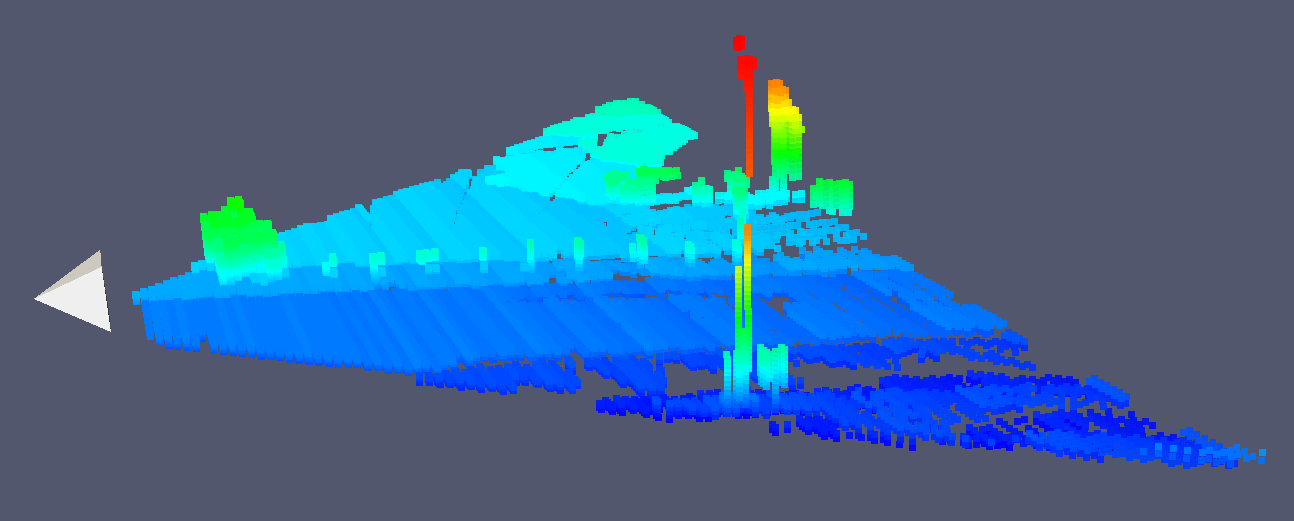
\includegraphics[width=14cm]{obrazky/occupied-frustum-with-camera-3}
\par\end{centering}
\caption{\label{fig:Occupied-samples-in}Occupied samples in frustum. Camera
is shown by white tetrahedron.}

\end{figure}


\subsection{Metrics and network setup}

Although the 3D map estimation is similar to the depth estimation
by the problem setup, it is more difficult since we try to infer occupancy
of occluded voxels, which was not an issue in depth prediction. Similarly
to the depth predictions, metrics for comparing different models and
optimizations of different loss functions are used. Compared to the
depth estimation where metrics were being calculated on images and
based on difference between predicted and ground truth depth, for
3D map estimation the classification based metrics are used since
this problem is by definition classification problem. 

In this setup of voxel-wise classification, we have 3 classes. Occupied,
free, and unknown voxels. Even for the setup of synthesizing 3D occupancy
grids, occupancy of some voxels is unknown. For instance, this happens
for car interior, occluded when viewed from all cameras and for space
below the road. During both training and validation, only known voxels
are used for loss calculation and metrics calculation. Let us recapitulate
usual terms used for classification problems with respect to this
particular problem. Voxel is false positive, if it is classified as
obstacle, but is free in ground truth. True positive voxel contains
obstacle in ground truth and is correctly classified as an obstacle.
True negative voxel is voxel without obstacle, a.k.a free voxel in
ground truth classified as free voxel in the prediction. And false
negative voxel is free in ground truth and in prediction. So number
of voxels in individual categories, which is then used in metrics,
can be expressed as
\begin{center}
\begin{tabular}{|c|c|c|}
\hline 
 & obstacle in ground truth & free in ground truth\tabularnewline
\hline 
\hline 
obstacle in prediction & $tp=\stackrel[i=1]{K}{\sum}1\left\{ obst\left(M_{i}\right)\land obst\left(M_{i}^{*}\right)\right\} $ & $fp=\stackrel[i=1]{K}{\sum}1\left\{ obst\left(M_{i}\right)\land free\left(M_{i}^{*}\right)\right\} $\tabularnewline
\hline 
free in prediction & $fn=\stackrel[i=1]{K}{\sum}1\left\{ free\left(M_{i}\right)\land obst\left(M_{i}^{*}\right)\right\} $ & $tn=\stackrel[i=1]{K}{\sum}1\left\{ free\left(M_{i}\right)\land free\left(M_{i}^{*}\right)\right\} $\tabularnewline
\hline 
\end{tabular}
\par\end{center}

where $obst\left(\cdot\right)$ is true for occupied voxels and $free\left(\cdot\right)$
is true for free voxels.

Following metrics are used:
\begin{enumerate}
\item False positive rate $fpr=\frac{fp}{fp+tn}$
\item True positive rate $fpr=\frac{tp}{fn+tp}$
\item Intersection over union $iou=\frac{\stackrel[i=1]{K}{\sum}1\left\{ obstacle\left(M_{i}\right)\land obstacle\left(M_{i}^{*}\right)\right\} }{\stackrel[j=1]{K}{\sum}1\left\{ obstacle\left(M_{j}\right)\lor obstacle\left(M_{j}^{*}\right)\right\} }$
\item L1 distance on known voxels $dist=\stackrel[i=1]{K}{\sum}1\left\{ known\left(M_{i}^{*}\right)\right\} \cdot|M_{i}-M_{i}^{*}|$
\end{enumerate}
where $M_{i}$ is $i$-th voxel in predicted voxelmap $M$, $M_{i}^{*}$
is $i$-th voxel in ground truth voxelmap $M^{*}$, $K$ is number
of voxels in voxelmap, $known\left(\cdot\right)$ is predicate true
for free or obstacle voxels. 

Also the loss function is different from depth estimation. The weighted
logistic loss is used. This is voxel-wise, because there can be multiple
occupied voxels per pixel and thus does not make sense to use the
loss function from depth estimation. The loss function is same as
in Zimmermann et al. \cite{zimmerman-active} and is as follows
\begin{equation}
L=-\left[\stackrel[i=1]{K}{\sum}w_{i}\log\left(1+\exp\left\{ -M_{i}M_{i}^{*}\right\} \right)\right]\label{eq:logistic-loss}
\end{equation}
where $M_{i}$ is value of $i$-th voxel in predicted voxelmap, $M_{i}^{*}$
is value of $i$-th voxel in ground truth voxelmap and $w_{i}$ is
weight of $i$-th voxel. The value of voxel in ground truth voxelmap
is as follows: $M_{i}^{*}=1$ for voxels with obstacles, $M_{i}^{*}=-1$
for free voxels. The weight $w_{i}$ serves two purposes. The first
purpose is masking out unknown voxels. The second purpose is to solve
the imbalanced classes issue. There are more free voxels than occupied
voxels, thus minimizing the sum per all voxels would lead to favouring
more frequent voxels. In this case, that would be free voxels and
thus it could learn to ignore some obstacles. The weighting modifies
the loss so all weights sum to 1 and weights per each class sum to
$\frac{1}{2}$. The weight $w_{i}$ for $i$-th voxel is defined as
follows. $w_{i}=0$ if $i$-th voxel in ground truth is unknown. $w_{i}=\frac{1}{2\cdot\#\,free\,voxels}$
if $i$-th voxel is free and $w_{i}=\frac{1}{2\cdot\#\,occupied\,voxels}$
if $i$-th voxel is occupied. 

The implementation of the neural network is publicly available at
\url{https://github.com/racinmat/depth-voxelmap-estimation}.

\chapter{Experiments}

\section{\label{subsec:Reverse-engineering}Reverse engineering the true Far
Clip}

For reverse engineering the far clip, I gathered 33293 screenshots
with parameters for projection matrix reconstruction and projection
matrices. Because during whole data gathering none of the parameters
used to reconstruct projection matrix, was changed, the projection
matrix should be same for all records. As mentioned in \ref{subsec:Camera-to-NDC}
parameters for reconstructing the Projection matrix are near clip,
far clip, screen width, screen height and field of view.

The screenshot contain both RGB images and depth buffer from GPU.

\begin{figure}
\begin{centering}
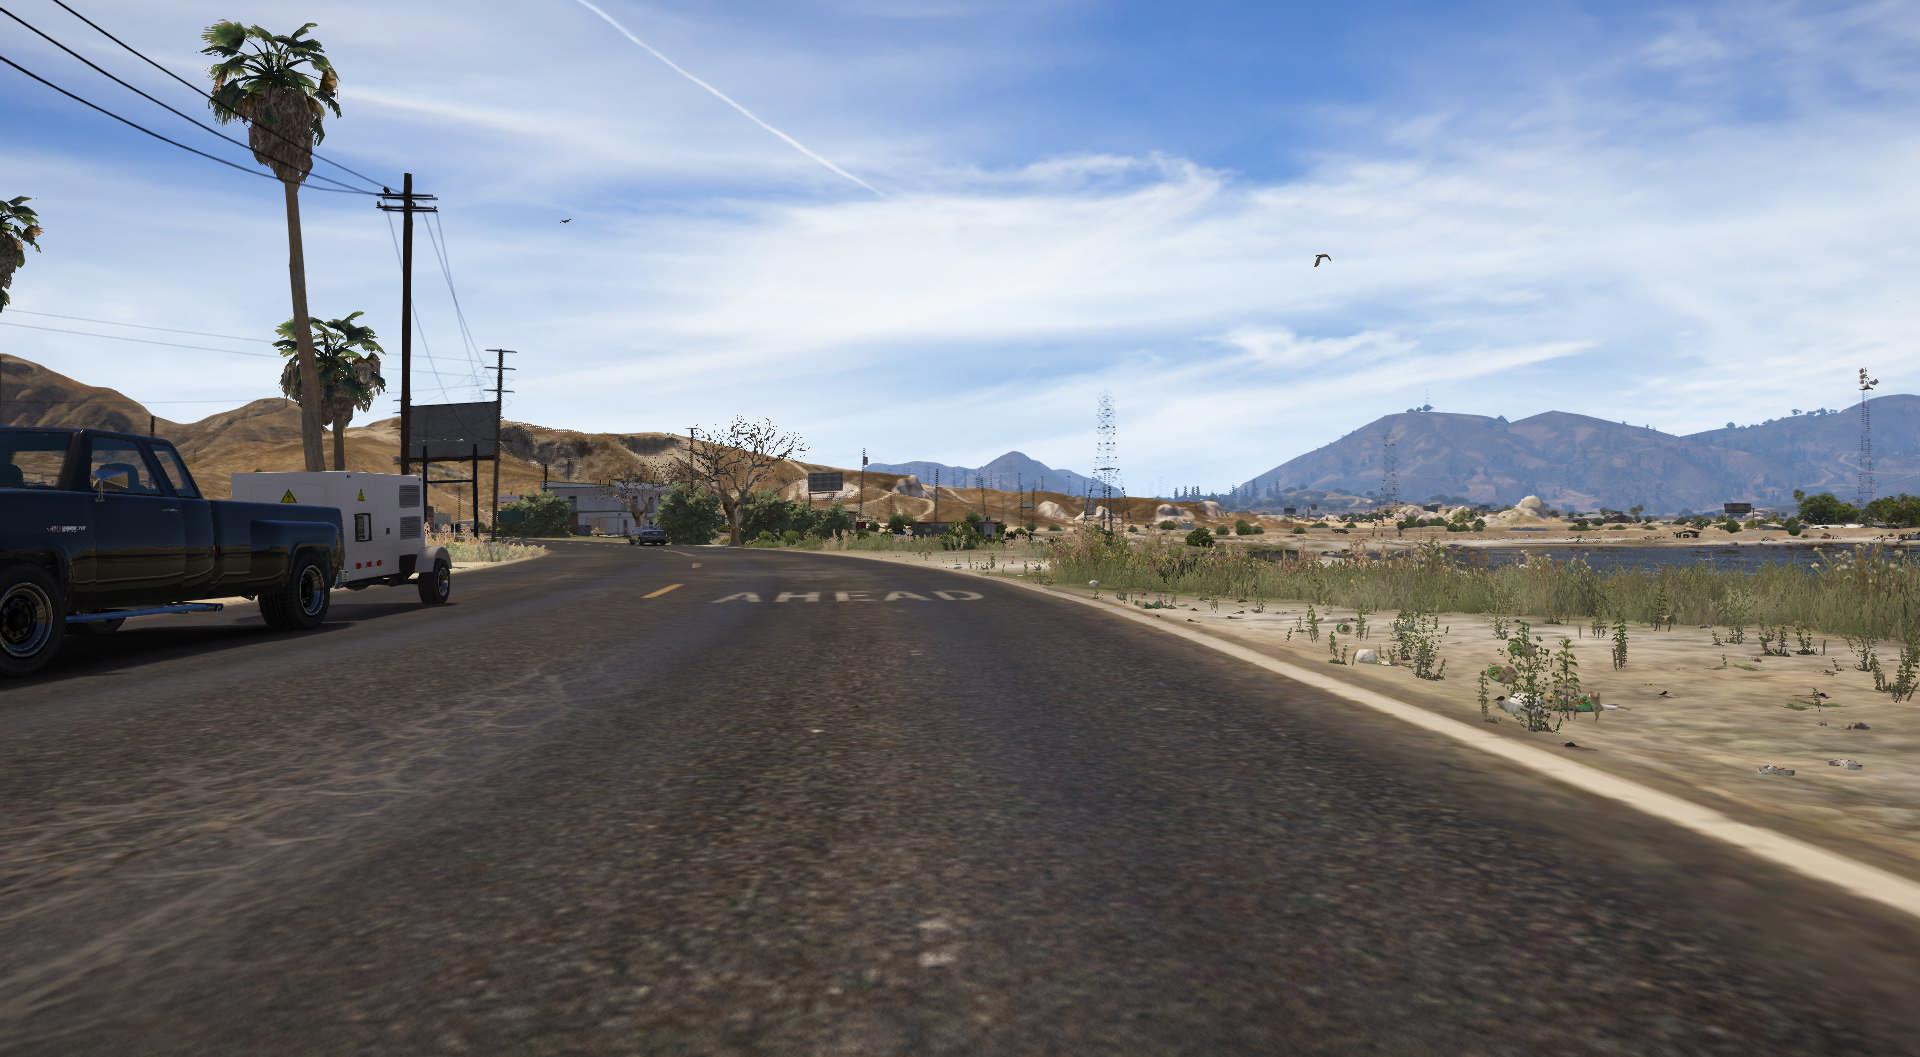
\includegraphics[scale=0.2]{obrazky/2018-03-30--06-00-56--114}
\par\end{centering}
\caption{\label{fig:Example-of-RGB}Example of RGB image}
\end{figure}
\begin{figure}
\begin{centering}
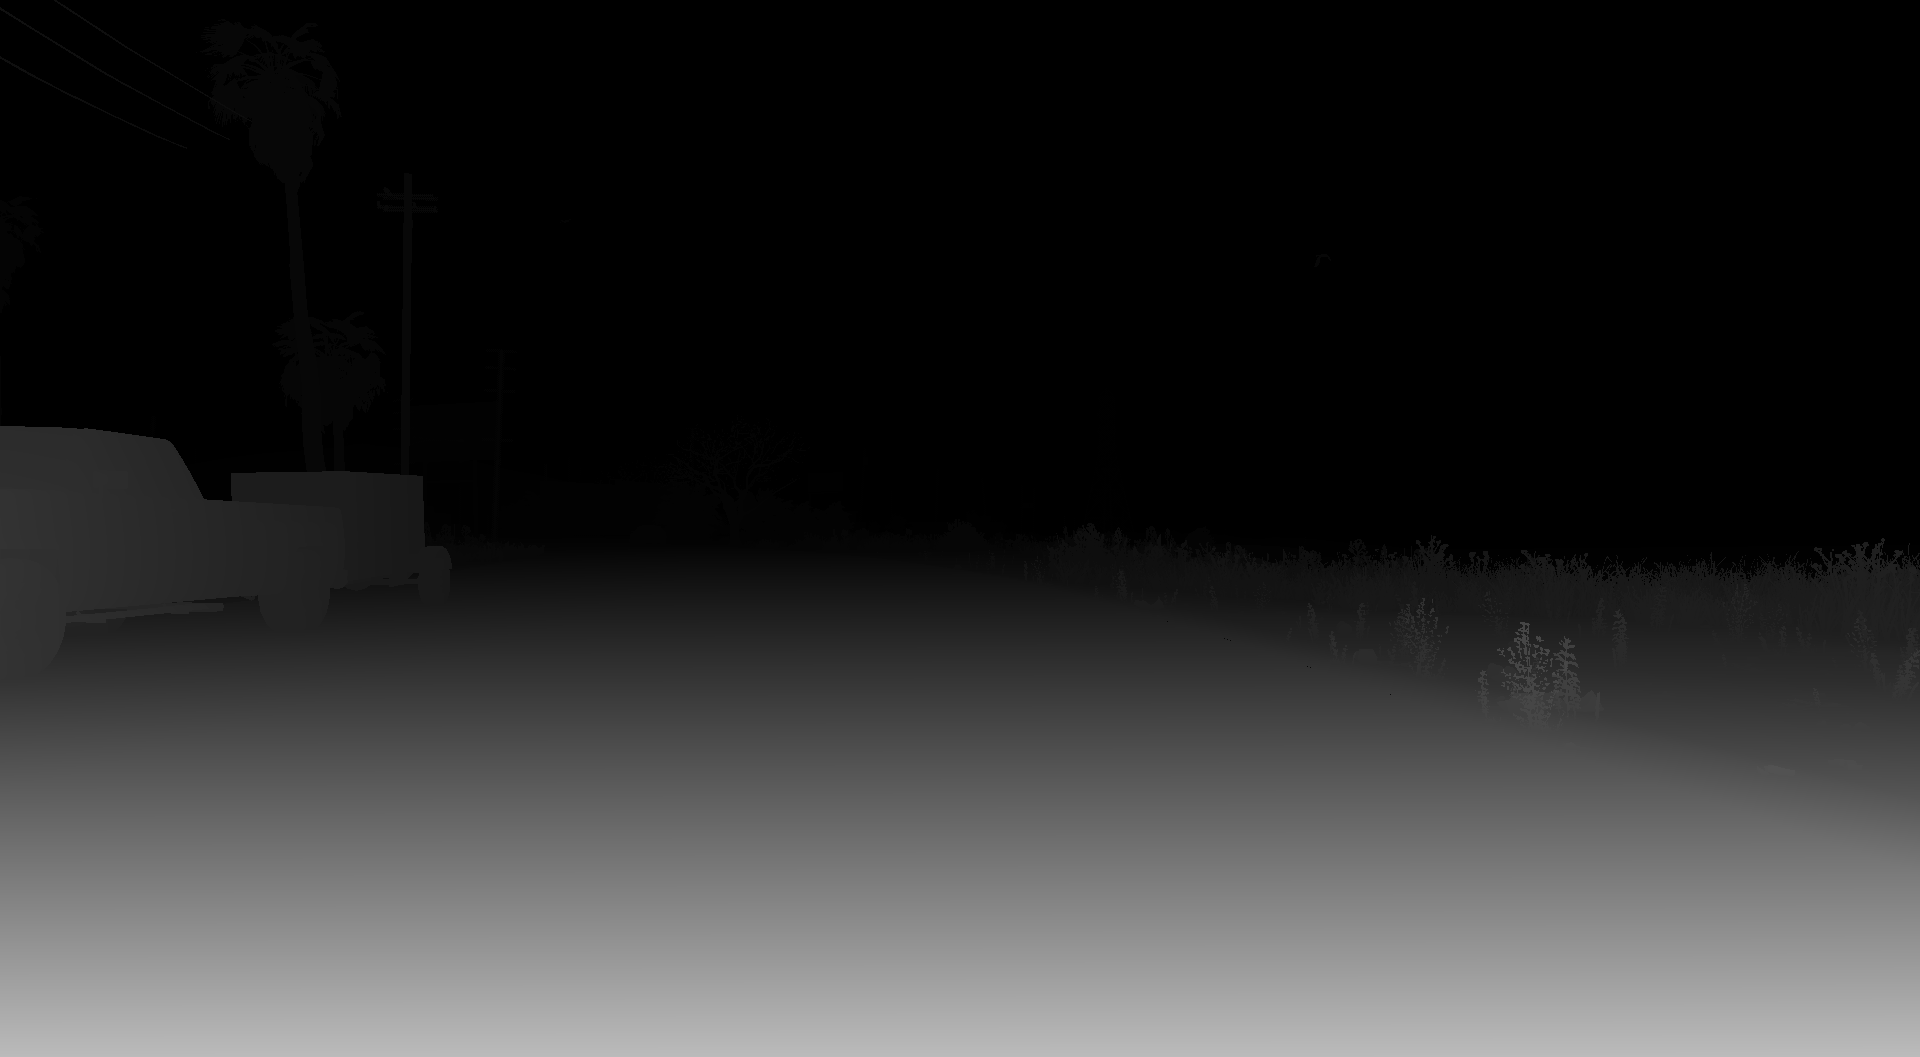
\includegraphics[scale=0.2]{obrazky/2018-03-30--06-00-56--114-depth-8bit-rescaled}
\par\end{centering}
\caption{\label{fig:Example-of-depth}Example of depth buffer}

\end{figure}

The projection matrix transforms frustum into cuboid. Open frameworks
have publicly available projection matrices, but RAGE does not have
publicly available any information about projection matrix, so in
order to obtain true far clip, I needed to reverse-engineer the mathematical
description of the projection matrix. For approximate estimation of
projection matrix parameters, I used DirectX projection matrix\cite{real-time-rendering}
as a starting point for analysis, because GTA V requires DirectX,
so I assumed it is underlying framework of RAGE.

The DirectX projection matrix is 
\[
P^{DirectX}=\begin{bmatrix}\frac{2n}{r-l} & 0 & -\frac{r+l}{r-l} & 0\\
0 & \frac{2n}{t-b} & -\frac{t+b}{t-b} & 0\\
0 & 0 & \frac{f}{f-n} & -\frac{fn}{f-n}\\
0 & 0 & 1 & 0
\end{bmatrix}
\]

where $n$ is near clip, $f$ is far clip, $l$ and $r$ determine
distance between left and right planes of the frustum and $t$ and
$b$ determine distance between top and bottom planes.

The view frustum is symmetric, so $r=-l$ and $t=-b$ \cite{real-time-rendering}.
In that case, the projection matrix is simplified to form
\[
P^{formal}=\begin{bmatrix}\frac{2n}{r+r} & 0 & -\frac{r-r}{r+r} & 0\\
0 & \frac{2n}{t+t} & -\frac{t-t}{t+t} & 0\\
0 & 0 & \frac{f}{f-n} & -\frac{fn}{f-n}\\
0 & 0 & 1 & 0
\end{bmatrix}=\begin{bmatrix}\frac{n}{r} & 0 & 0 & 0\\
0 & \frac{n}{t} & 0 & 0\\
0 & 0 & \frac{f}{f-n} & -\frac{fn}{f-n}\\
0 & 0 & 1 & 0
\end{bmatrix}
\]
The DirectX maps near clip to 0 and far clip to 1, but from data,
where obviously\ref{fig:Example-of-depth} nearer pixels had higher
value in depth buffer than pixel more far from camera, I concluded
that near and far clip are being mapped to 1 and 0, respectively.
The far clip being mapped to 0 can also be deduced by pixels for sky
having 0 value.

Due to this fact, we switch the near and clip in the matrix formal
description

\[
P^{formal}=\begin{bmatrix}\frac{f}{r} & 0 & 0 & 0\\
0 & \frac{f}{t} & 0 & 0\\
0 & 0 & \frac{n}{n-f} & -\frac{fn}{n-f}\\
0 & 0 & 1 & 0
\end{bmatrix}
\]

The example in \ref{fig:Example-of-depth} does not have actual depth
buffer values, but instead, it is rescaled visualization. Since the
depth buffer pixels are in range $\left[0,1\right]$ and PNG images
take unsigned 8bit integer, this image is mapped linearly from $\left[0,1\right]$
to $\left[0,255\right]$. Since even the nearest pixels were distant
from near clip and real range of pixels in this image was $\left[0,19\right]$,
I rescaled it 10 times to range $\left[0,190\right]$, so the depth
is visible.

At first, I assumed the camera near clip and far clip obtained by
native calls \ref{native-call-near-clip} and the projection matrix
is same as in DirectX. 

The near clip and far clip calculation can be demonstrated on image
\ref{fig:Example-of-RGB}. 

By calling CAM::GET\_CAM\_NEAR\_CLIP$=n_{c}$ and CAM::GET\_CAM\_FAR\_CLIP$=f_{c}$
I obtained values $n_{c}=1.5$ and $f_{c}=800$. I also obtained projection
matrix calculated by method described in \ref{subsec:Rendering-pipeline-data},
which is 
\[
P^{real}=\begin{bmatrix}1.210067 & 0 & 0 & -0.000004\\
0 & 2.144507 & 0 & 0.000002\\
0 & 0 & 0.00015 & 1.500225\\
0 & 0 & -1 & 0
\end{bmatrix}
\]

In the formalization of the matrix, $P_{formal}$, there are 4 variables.
$r$ and $t$ appear only in one element of matrix, so they can be
verified only after reverse engineering the far clip. From the $P_{2,2}^{formal}$
and $P_{2,3}^{formal}$, I can calculate the near and far clip by
\begin{align*}
P_{2,2}^{formal} & =\frac{n}{n-f}\\
nP_{2,2}^{formal}-fP_{2,2}^{formal} & =n\\
\frac{n\left(P_{2,2}^{formal}-1\right)}{P_{2,2}^{formal}} & =f
\end{align*}

\begin{align*}
P_{2,3}^{formal} & =-\frac{fn}{n-f}\\
P_{2,3}^{formal}\left(n-f\right) & =-fn\\
nP_{2,3}^{formal} & =f\left(P_{2,3}^{formal}-n\right)\\
\frac{nP_{2,3}^{formal}}{\left(P_{2,3}^{formal}-n\right)} & =f
\end{align*}
\begin{align*}
\frac{nP_{2,3}^{formal}}{\left(P_{2,3}^{formal}-n\right)} & =\frac{n\left(P_{2,2}^{formal}-1\right)}{P_{2,2}^{formal}}\\
P_{2,3}^{formal}P_{2,2}^{formal} & =\left(P_{2,2}^{formal}-1\right)\left(P_{2,3}^{formal}-n\right)\\
\frac{P_{2,3}^{formal}P_{2,2}^{formal}}{P_{2,2}^{formal}-1} & =P_{2,3}^{formal}-n\\
P_{2,3}^{formal}-\frac{P_{2,3}^{formal}P_{2,2}^{formal}}{P_{2,2}^{formal}-1} & =n\\
-\frac{P_{2,3}^{formal}}{P_{2,2}^{formal}-1} & =n
\end{align*}

\begin{align*}
\frac{\left(-\frac{P_{2,3}^{formal}}{P_{2,2}^{formal}-1}\right)\left(P_{2,2}^{formal}-1\right)}{P_{2,2}^{formal}} & =f\\
-\frac{P_{2,3}^{formal}}{P_{2,2}^{formal}} & =f
\end{align*}

From these calculations, we can calculate near and far clip as 
\begin{align*}
n & =-\frac{P_{2,3}^{formal}}{P_{2,2}^{formal}-1}=-\frac{1.500225}{0.00015-1}=1.500225\\
f & =-\frac{P_{2,3}^{formal}}{P_{2,2}^{formal}}=-\frac{1.500225}{0.00015}=-10001.5
\end{align*}

From these calculations we can see the third column of the projection
matrix has incorrect sign, because the $P_{3,2}^{formal}$ should
be 1 and instead it is -1, and the far clip is negative, which should
not be. When changing signs of third column of projection matrix,
we obtain following formal definition of projection matrix. That sign
switching means the view frustum is in opposite direction of Z axis.
\[
P^{formal}=\begin{bmatrix}\frac{f}{r} & 0 & 0 & 0\\
0 & \frac{f}{t} & 0 & 0\\
0 & 0 & -\frac{n}{n-f} & -\frac{fn}{n-f}\\
0 & 0 & -1 & 0
\end{bmatrix}
\]

After fixing the sign issue, the relationship between $P^{formal}$
and clips is

\begin{align*}
\frac{P_{2,3}^{formal}}{P_{2,2}^{formal}+1} & =n=\frac{1.500225}{0.00015+1}=1.499999\\
\frac{P_{2,3}^{formal}}{P_{2,2}^{formal}} & =f=\frac{1.500225}{0.00015}=10001.5
\end{align*}

As we can see, the $n=1.499999\approx n_{c}=1.5$ so for near clip,
we can say we successfully reverse-engineered the relation between
the projection matrix and the near clip. The far clip, on the other
hand, differs $f=10001.5\neq f_{c}=800$. The difference is very high,
which lead us to assumption that there is some new far clip, which
is not same as obtained through API, $f_{c}$. 

The other check we can perform is projecting points laying on near
clip and far clip into NDC space. 

We prepare two points. Because of many zero elements in $P^{formal}$,
we can see $x$-axis and $y$-axis don't affect the $z$-axis of projected
point. Thus I prepared two points:
\[
\begin{bmatrix}1 & 1\\
1 & 1\\
-1.5 & -800\\
1 & 1
\end{bmatrix}
\]
, which are laying on the near clip and far clip, respectively. We
would assume that they would be mapped to 1 and 0, respectively. The
negative sign is here because in RAGE, the camera view frustum is
in negative part of Z axis.

\[
\begin{bmatrix}1.210067 & 0 & 0 & -0.000004\\
0 & 2.144507 & 0 & 0.000002\\
0 & 0 & 0.00015 & 1.500225\\
0 & 0 & -1 & 0
\end{bmatrix}\begin{bmatrix}1 & 1\\
1 & 1\\
-0.15 & -800\\
1 & 1
\end{bmatrix}=\begin{bmatrix}1.210063 & 1.210063\\
2.144509 & 2.144509\\
1.5 & 1.380225\\
1.5 & 800
\end{bmatrix}
\]
by normalization we obtain 
\[
\begin{bmatrix}\frac{1.210063}{1.5} & \frac{1.210063}{800}\\
\frac{2.144509}{1.5} & \frac{2.144509}{800}\\
\frac{1.50045}{1.5} & \frac{1.620225}{800}\\
\frac{1.5}{1.5} & \frac{800}{800}
\end{bmatrix}=\begin{bmatrix}0.80670867 & 0.00151258\\
1.42967267 & 0.00268064\\
1 & 0.00172528\\
1 & 1
\end{bmatrix}
\]
from which we can see the near clip $n_{c}$ is being projected correctly,
but far clip $f_{c}$ is not being projected into 0 and that true
far clip $f$ is behind this far flip $f_{c}$. These calculations
give us some insight into projection matrix and its role in far clip
estimation, but for more robust estimate, I analysed all 33293 matrices.
In GTA, matrices are not gathered correctly every time and in some
cases, resulting matrices are unusable. Because I knew the near clip
precisely, I discarded all matrices, with calculated near clip with
difference from real near clip $>10^{-4}$. For the rest of matrices,
I calculated near clip and far clip for each of them. In the figure
\ref{fig:Frequencies-of-} can be seen histograms of these calculated
far clip and near clip for each matrix, respectively. Even near clip
values, which we know precisely, differ, but with very little variance,
in range $\left[1.5003,1.50048\right]$ which means difference from
true near clip in range $\left[3\cdot10^{-4},4.8\cdot10^{-4}\right]$
which is simply explained by numerical instability. Both histograms
have logarithmic y scale, so we easily see which value occurs more
frequently. The value $-10003.814$ occurred most frequently in matrices,
one and half order of magnitude more frequently than second frequent
value, and this value also corresponds to the median of all calculated
far clips. Thus this far clip $F=-10003.814$ has been used in all
later experiments as a true far clip.

\begin{figure}
\begin{centering}
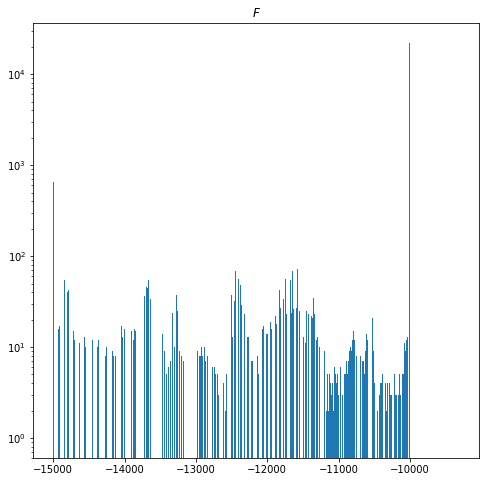
\includegraphics[width=6cm]{obrazky/far-clip-f}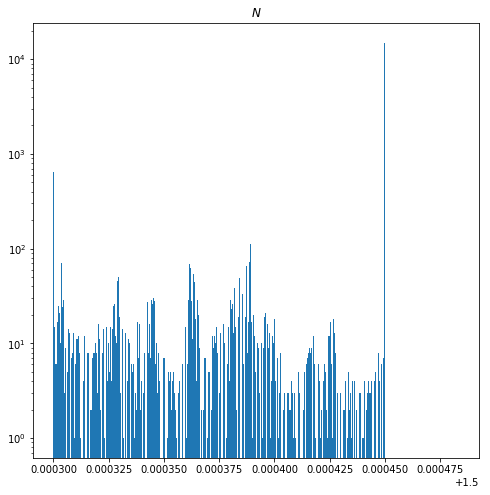
\includegraphics[width=6cm]{obrazky/far-clip-n}
\par\end{centering}
\caption{\label{fig:Frequencies-of-}Frequencies of $P_{2,2}$ and $P_{2,3}$}

\end{figure}


\section{Depth estimation}

For all experiments, the same network architecture has been used,
only hyper-parameters were being tuned. The initial experiments started
with 201 depth bins, as used in \cite{depth-estimation-hierarchical-fusion-soft-weighting}
but with additional depth bin for more distant depth values. But the
network failed to learn in this setup. The cost increased exponentially
instead of decreasing, as can be seen in figure \ref{fig:Failing-to-learn}.
The cost function which was being minimized in this setup was the
multinomial loss, as described in \ref{eq:loss-multinomial}. With
time, cost function was increasing. In the run denoted by light blue
colour, only 40 training images were fed into the network, to try
if it is able to remember patterns, without any requirement of generalization.
As can be seen, even in this setup network failed to learn. All runs
are runs with different learning rates, in expectation that lower
learning rate would prevent this cost explosion, but it did not seem
to have any effect at all. The training and validation data from dataset
were split in 80/20 ratio.

\begin{figure}
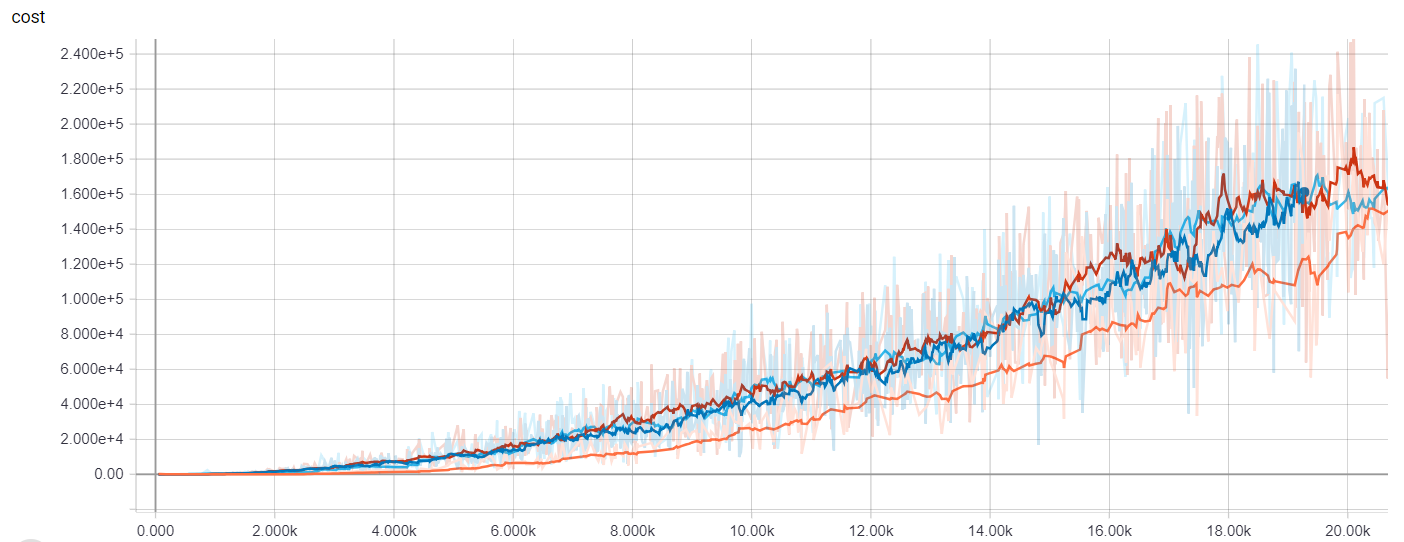
\includegraphics[width=14cm]{obrazky/initial-learn-fail.PNG}

\caption{\label{fig:Failing-to-learn}Failing to learn}
\end{figure}
After reducing the output number of depth levels to 101, 100 depth
levels and one remaining level for all depth values outside the binned
range, network started to learn, as. The training was then run in
multiple setups, to find the best predictor. 9 setups will be discussed.
Setups parameters can be seen in the table \ref{tab:Depth-estimation-setups}.
As a loss function, the information gain based loss in \ref{eq:loss-infogain}
has been used. The initial learning rate is same for all setups. The
Nadam optimizer is abbreviation for Adam optimizer with Nesterov momentum.
For all runs using Adam and Nadam optimizers, only epsilon parameter
was tuned, beta1 and beta2 parameters were constant, beta1=$0.9$,
beta2=$0.999$. The SGDN is abbreviation for the stochastic gradient
descent with Nesterov momentum.The initial learning rate was set to
$10^{-4}$for all runs. For setups 1 to 6, learning rate decay has
been used. The learning rate decay is staircase, after a period given
in ``decay after'' column the learning rate is divided by 10. For
runs 7 to 9, learning rate remained unchanged for all training. Networks
were trained on different GPUs, namely, Nvidia Titan Xp, Titan X,
and Nvidia GTX 1080Ti. Due to different computation capability of
these cards and different number of CUDA cores, run times are not
highly correlated with number of iterations.

\begin{table}
\begin{tabular}{|c|c|c|c|c|}
\hline 
name & optimizer & decay after & \multirow{1}{*}{training time} & iterations\tabularnewline
\hline 
\hline 
setup 1 & Adam(epsilon=$10^{-8}$) & $2\cdot10^{4}$ steps & 58h & 237k\tabularnewline
\hline 
setup 2 & Adam(epsilon=$10^{-8}$) & $3\cdot10^{4}$ steps & 26h & 164k\tabularnewline
\hline 
setup 3 & Nadam(epsilon=$10^{-8}$) & $3\cdot10^{4}$ steps & 26h & 105k\tabularnewline
\hline 
setup 4 & Adam(epsilon=$10^{-5}$) & $3\cdot10^{4}$ steps & 26h & 175k\tabularnewline
\hline 
setup 5 & Nadam(epsilon=$10^{-5}$) & $3\cdot10^{4}$ steps & 30h & 202k\tabularnewline
\hline 
setup 6 & Nadam(epsilon=$10^{-2}$) & $3\cdot10^{4}$ steps & 30h & 189k\tabularnewline
\hline 
setup 7 & Nadam(epsilon=$10^{-8}$) & no decay & 30h & 120k\tabularnewline
\hline 
setup 8 & SGDN(momentum=$0.999$) & no decay & 26h & 184k\tabularnewline
\hline 
setup 9 & SGDN(momentum=$0.9$) & no decay & 26h & 108k\tabularnewline
\hline 
\end{tabular}

\caption{\label{tab:Depth-estimation-setups}Depth estimation setups}
\end{table}
Metrics for depth estimation and loss have been calculated for the
validation dataset on these 9 setups, they can be seen in table \ref{tab:Depth-estimation-metrics}.
The accuracy under threshold $1.25$ ($aut\left(1.25\right)$) is
in range $\left[0,1\right]$ by definition. 0 accuracy means depth
in not pixel is in range from $\frac{1}{1.25}=0.5$ to $1.25$ of
ground truth depth, 1 accuracy means all pixels are in $0.8$ to $1.25$
of ground truth depth. All these calculations are done on reconstructed
images, meaning higher accuracy means better models. Error metrics
measure error rate and thus lower error means better model. Some metrics
highly correlate with each other, showing they describe similar information.
From accuracy under threshold and root mean squared log error ($rmls$)
we can see setups 6,8,9 perform far worse than other models. So we
can see generally SGDN performed worse than Adam and Nadam optimizers.
From Adam and Nadam optimizers, the setup 7 performed the best, which
is Nadam optimizer with epsilon=$10^{-8}$ and without the learning
decay. That can be seen in all metrics except of mean relative error. 

\begin{table}
\begin{tabular}{|c|c|c|c|c|c|c|}
\hline 
name & $aut\left(1.25\right)$ & mean relative error & $rms$ & $rmls$ & average $\log_{10}$ error & loss\tabularnewline
\hline 
\hline 
setup 1 & 0.4390 & 0.3607 & 10.7808 & 0.5415 & 0.2880 & 14.6054\tabularnewline
\hline 
setup 2 & 0.4393 & 0.3432 & 11.0467 & 0.5533 & 0.2926 & 14.5629\tabularnewline
\hline 
setup 3 & 0.4554 & 0.3287 & 10.3699 & 0.5219 & 0.2730 & 14.5234\tabularnewline
\hline 
setup 4 & 0.4258 & 0.3392 & 9.7831 & 0.4849 & 0.2620 & 14.5913\tabularnewline
\hline 
setup 5 & 0.4314 & 0.3394 & 10.2730 & 0.5066 & 0.2708 & 14.6061\tabularnewline
\hline 
setup 6 & 0.0390 & 0.6588 & 13.8523 & 0.8978 & 0.6960 & 14.8873\tabularnewline
\hline 
setup 7 & 0.4852 & 0.3494 & 8.2342 & 0.4140 & 0.2180 & 14.5132\tabularnewline
\hline 
setup 8 & 0.0 & 0.7106 & 13.9028 & 0.9403 & 0.7651 & 14.9104\tabularnewline
\hline 
setup 9 & 0.0508 & 0.6488 & 13.8551 & 0.8948 & 0.6873 & 14.8796\tabularnewline
\hline 
\end{tabular}

\caption{\label{tab:Depth-estimation-metrics}Depth estimation metrics}
\end{table}

Few images from the validation dataset and their depth predictions
can be seen in figure \ref{fig:Depth-estimation-samples}. In the
first row, we can see the RGB image, in the second row is the ground
truth depth in meters. The third row depicts ground truth images reconstructed
by the soft-sum inference from depth level bins. Here we can see all
information behind 50 meters in truncated, which also visually helps
us to focus on near objects. The red colour is for nearer objects
and blue colour is for more distant objects. In rows 4-7 we can see
the predictions of setups 3, 4, 5 and 7 which are performing better
than rest of setups. 

\begin{figure}
\begin{centering}
\begin{tabular}{>{\centering}p{2cm}ccc>{\centering}p{2cm}}
\multicolumn{1}{c}{RGB image} & \vspace{0pt}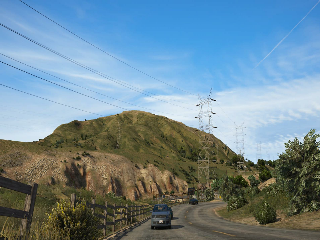
\includegraphics[width=3.5cm]{obrazky/depths/orig-rgb-1} & \vspace{0pt}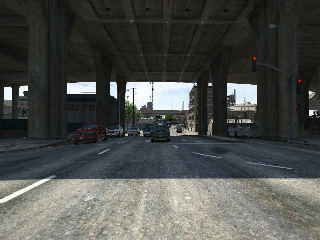
\includegraphics[width=3.5cm]{obrazky/depths/orig-rgb-4} & \vspace{0pt}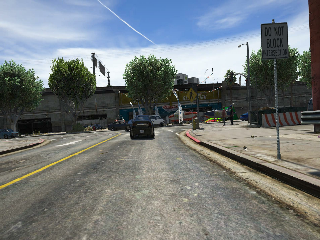
\includegraphics[width=3.5cm]{obrazky/depths/orig-rgb-3} & \tabularnewline
\multicolumn{1}{>{\centering}p{2cm}}{original depth} & \vspace{0pt}\includegraphics[width=3.5cm]{obrazky/depths/colored-orig-depth-1\lyxdot png} & \vspace{0pt}\includegraphics[width=3.5cm]{obrazky/depths/colored-orig-depth-4\lyxdot png} & \vspace{0pt}\includegraphics[width=3.5cm]{obrazky/depths/colored-orig-depth-3\lyxdot png} & 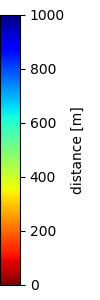
\includegraphics[height=3cm]{obrazky/depths/colorbar-orig}\tabularnewline
\multicolumn{1}{>{\centering}p{2cm}}{truncated depth} & \vspace{0pt}\includegraphics[width=3.5cm]{obrazky/depths/colored-gt-depth-1\lyxdot png} & \vspace{0pt}\includegraphics[width=3.5cm]{obrazky/depths/colored-gt-depth-4\lyxdot png} & \vspace{0pt}\includegraphics[width=3.5cm]{obrazky/depths/colored-gt-depth-3\lyxdot png} & 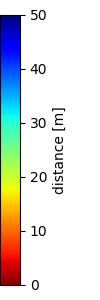
\includegraphics[height=3cm]{obrazky/depths/colorbar-cropped}\tabularnewline
\multicolumn{1}{>{\centering}p{2cm}}{setup 3} & \vspace{0pt}\includegraphics[width=3.5cm]{obrazky/depths/colored-predicted-1-2018-04-01--00-26-49\lyxdot png} & \vspace{0pt}\includegraphics[width=3.5cm]{obrazky/depths/colored-predicted-4-2018-04-01--00-26-49\lyxdot png} & \vspace{0pt}\includegraphics[width=3.5cm]{obrazky/depths/colored-predicted-3-2018-04-01--00-26-49\lyxdot png} & 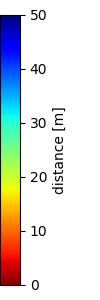
\includegraphics[height=3cm]{obrazky/depths/colorbar-cropped}\tabularnewline
\multicolumn{1}{>{\centering}p{2cm}}{setup 4} & \vspace{0pt}\includegraphics[width=3.5cm]{obrazky/depths/colored-predicted-1-2018-04-01--00-32-39\lyxdot png} & \vspace{0pt}\includegraphics[width=3.5cm]{obrazky/depths/colored-predicted-4-2018-04-01--00-32-39\lyxdot png} & \vspace{0pt}\includegraphics[width=3.5cm]{obrazky/depths/colored-predicted-3-2018-04-01--00-32-39\lyxdot png} & \includegraphics[height=3cm]{obrazky/depths/colorbar-cropped}\tabularnewline
\multicolumn{1}{>{\centering}p{2cm}}{setup 5} & \vspace{0pt}\includegraphics[width=3.5cm]{obrazky/depths/colored-predicted-1-2018-04-02--02-51-28\lyxdot png} & \vspace{0pt}\includegraphics[width=3.5cm]{obrazky/depths/colored-predicted-4-2018-04-02--02-51-28\lyxdot png} & \vspace{0pt}\includegraphics[width=3.5cm]{obrazky/depths/colored-predicted-3-2018-04-02--02-51-28\lyxdot png} & \includegraphics[height=3cm]{obrazky/depths/colorbar-cropped}\tabularnewline
\multicolumn{1}{>{\centering}p{2cm}}{setup 7} & \vspace{0pt}\includegraphics[width=3.5cm]{obrazky/depths/colored-predicted-1-2018-04-02--02-59-31\lyxdot png} & \vspace{0pt}\includegraphics[width=3.5cm]{obrazky/depths/colored-predicted-4-2018-04-02--02-59-31\lyxdot png} & \vspace{0pt}\includegraphics[width=3.5cm]{obrazky/depths/colored-predicted-3-2018-04-02--02-59-31\lyxdot png} & \includegraphics[height=3cm]{obrazky/depths/colorbar-cropped}\tabularnewline
\end{tabular}
\par\end{centering}
\caption{\label{fig:Depth-estimation-samples}Depth estimation samples}

\end{figure}

\begin{figure}
\includegraphics[width=14cm]{obrazky/depth-cost}

\caption{\label{fig:Training-for-depth-loss}Training for depth estimation
- loss}
\end{figure}
\begin{figure}
\includegraphics[width=8cm]{obrazky/depth-root_mean_log_square_error}\includegraphics[width=8cm]{obrazky/depth-mean_relative_error}

\includegraphics[width=8cm]{obrazky/depth-root_mean_square_error}\includegraphics[width=8cm]{obrazky/depth-under_treshold_1\lyxdot 25}

\caption{\label{fig:Training-for-depth-metrics}Training for depth estimation
- metrics}

\end{figure}

In the figure \ref{fig:Training-for-depth-loss} we can see the loss
during training and in figure \ref{fig:Training-for-depth-metrics}
we can see all metrics gathered during training. Interesting property
of loss function based on information gain is the fact that it does
not seem to converge most of the time during training, but all metrics
are being optimized even when it is not seen in the loss figure. Here
we can see clearly how setups 6, 8 and 9 performed poorly and setup
7 performed the best in all metrics. The setup 7, which is Adam optimizer
with Nesterov momentum, a.k.a. Nadam optimizer with constant learning
rate seems to have best results and thus is used as a default optimizer
for 3D map estimation and learning rate is constant in all setups.

\section{3D map estimation}

For 3D map estimation, I also trained multiple setups and evaluated
them, 7 of them with most promising results are discussed here. The
architecture was being modified, the last softmax layer was removed
because now we don't aim to predict occupation of only 1 depth voxel
per pixel, but we can predict multiple occupied voxels. Also, for
setups 5, 6 and 7, new deconvolutional layer was stacked, between
the last convolutional layer and the deconvolutional layer before
the output. The parameters for optimizer were same, epsilon=$10^{-8}$,
beta1=$0.9$, beta2=$0.999$ for Nadam optimizer, and momentum=$0.9$
was used for SGD optimizer with Nesterov momentum. For all setups,
the weighted logistic loss \ref{eq:logistic-loss} is used. We can
see the overview in the figure \ref{tab:3d-estimation-setups}. Then
I evaluated these setups on validation sets and reported results in
the table \ref{tab:3d-estimation-metrics}.

\begin{table}
\begin{tabular}{|c|c|c|c|c|c|}
\hline 
name & loss & optimizer & new deconvolutional layer & \multirow{1}{*}{training time} & iterations\tabularnewline
\hline 
\hline 
setup 1 & logistic & Nadam & - & 25h & 141k\tabularnewline
\hline 
setup 2 & logistic & SGDN & - & 24h & 150k\tabularnewline
\hline 
setup 3 & logistic & Nadam & kernel=5, stride=1,out\_dim=50 & 28h & 147k\tabularnewline
\hline 
setup 4 & logistic & Nadam & kernel=2, stride=2,out\_dim=50 & 44h & 187k\tabularnewline
\hline 
setup 5 & logistic & Nadam & kernel=2, stride=2,out\_dim=200 & 52h & 154k\tabularnewline
\hline 
\end{tabular}

\caption{\label{tab:3d-estimation-setups}3D estimation setups}
\end{table}

\begin{table}
\begin{tabular}{|c|c|c|c|c|c|}
\hline 
name & false positive rate & true positive rate & intersection over union & $l_{1}$ distance & loss\tabularnewline
\hline 
\hline 
setup 1 & 0.2732 & 0.8603 & 0.6523 & 12151.0 & 0.1244\tabularnewline
\hline 
setup 2 & 0.0505 & 0.4712 & 0.2214 & 64437.4 & 0.13013582\tabularnewline
\hline 
setup 3 & 0.2120 & 0.8369 & 0.6233 & 13386.8 & 0.1080089\tabularnewline
\hline 
setup 4 & 0.2250 & 0.8355 & 0.6192 & 13587.4 & 0.097417\tabularnewline
\hline 
setup 5 & 0.2356 & 0.8514 & 0.6730 & 12359.5 & 0.123826\tabularnewline
\hline 
\end{tabular}

\caption{\label{tab:3d-estimation-metrics}Depth estimation metrics}
\end{table}

The process of training is shown in figures \ref{fig:Training-for-3d-loss}
and \ref{fig:Training-for-3d-metrics}. In figure \ref{fig:Training-for-3d-loss}
we can see the cost being minimized. Here the logistic loss itself
shows how individual setups perform. The figure has logarithmic Y
scale for better visualization of individual setups. In the figure
\ref{fig:Training-for-3d-metrics} we can see metrics. The false positive
rate is very low for all runs, but for other metrics we can see stochastic
gradient descent with Nesterov momentum (setup 2) performed much poorer
than other run. On the other hand, the setup 1 and setup 5 perform
better than other setups in all metrics. From this we can than reduction
of 4th dimension to the size od 50 in the end of the network worsens
the performance, on the other hand, adding layer with 4th dimension
of size 400 performs better in intersection over union metric.

\begin{figure}
\includegraphics[width=14cm]{obrazky/3d-cost}

\caption{\label{fig:Training-for-3d-loss}Training for 3D map estimation -
loss}
\end{figure}
\begin{figure}
\includegraphics[width=8cm]{obrazky/3d-iou}\includegraphics[width=8cm]{obrazky/3d-l1_dist_on_known}

\includegraphics[width=8cm]{obrazky/3d-false_positive_rate}\includegraphics[width=8cm]{obrazky/3d-true_positive_rate}

\caption{\label{fig:Training-for-3d-metrics}Training for 3D map estimation
- metrics}
\end{figure}

In figure \ref{fig:3d-estimation-samples} we can see two sample images
from validation dataset, their ground truth voxelmaps and predicted
voxelmaps from 2 best setups, setup 1 and setup 5. In the first row,
we can see the input image to the network, in the second row is the
ground truth voxelmap in camera view frustum (and camera position
denoted by white tetrahedron), and the last two rows show predictions
of setup 1 and setup 5, respectively.

\begin{figure}
\begin{centering}
\begin{tabular}{>{\centering}p{2cm}cc}
\multicolumn{1}{c}{RGB image} & \vspace{0pt}\includegraphics[width=5.5cm]{obrazky/3ds/orig-rgb-2} & \vspace{0pt}\includegraphics[width=5.5cm]{obrazky/3ds/orig-rgb-1}\tabularnewline
\multicolumn{1}{c}{original voxelmap} & \vspace{0pt}\includegraphics[width=6cm]{obrazky/3ds/gt-2.PNG} & \vspace{0pt}\includegraphics[width=6cm]{obrazky/3ds/gt-1.PNG}\tabularnewline
\multicolumn{1}{c}{setup 1} & \vspace{0pt}\includegraphics[width=6cm]{obrazky/3ds/img-2-setup-0.PNG} & \vspace{0pt}\includegraphics[width=6cm]{obrazky/3ds/img-1-setup-0.PNG}\tabularnewline
\multicolumn{1}{c}{setup 5} & \vspace{0pt}\includegraphics[width=6cm]{obrazky/3ds/img-2-setup-5.PNG} & \vspace{0pt}\includegraphics[width=6cm]{obrazky/3ds/img-1-setup-5.PNG}\tabularnewline
\end{tabular}
\par\end{centering}
\caption{\label{fig:3d-estimation-samples}3D estimation samples}

\end{figure}


\chapter{Conclusion and Future Work}

This thesis contributed to the reactive depth and 3D estimation by
proposing a deep neural network architecture for depth and 3D estimation
from single RGB image. The trained neural network works well for roads-like
images with fixed camera field of view. The number of depth bins showed
to be essential for the ability of network to learn the depth estimation
correctly. In conclusion, I proposed neural network architecture for
both depth and 3D estimation and evaluated it with multiple hyper-parameters.
I demonstrated an automatic synthetic dataset creation and labels
gathering from rich virtual world of GTA V for dense labelling of
data. Then I reverse-engineered camera parameters and parameters of
RAGE visualization pipeline and described an API used to control the
virtual world and manipulate it during data gathering. I proposed
synthetic dataset gathered by aforementioned method and then used
this dataset for training neural network for depth and 3D map estimation
tasks. I compared multiple optimizers for depth estimation and evaluated
their performance. Adam optimizer with Nesterov momentum shown to
perform better than Adam optimizer, which is seen by many as a default
optimizer for most of tasks, and it also shown to perform better than
SGD optimizer with Nesterov momentum. Lastly, I trained neural network
for 3D map estimation and evaluated several network architecture changes.
Compressing the network capacity of the network in the end of the
structure from 101 dimension size to the dimension size of 50 and
back to 101 shown to worsen the accuracy, on the other hand increasing
the dimension size to 200 between last convolution layer and last
layer improved only union over intersection, but did not outperform
model without additional layer in other metrics.

During working with GTA V, many aspects have been discovered, but
even more of them remained to be discovered in the future. In GTA
V reverse-engineering, many stencil values semantics remain to be
interpreted. Also, in GTA V, the modding capabilities are far from
using their full potential. Lots of existing mods could help with
scenarios setup for gathering data in specific situations, also necessary
tooling needs to be developed to provide simple interface for scenarios
setup. But probably one of the most promising mod categories are visual
mods, which enhance the graphics of the game. Many visual mods are
being used currently and some of them can be combined together, utilizing
advantages of them both. The main difficulty in using visual mods
is evaluation of their photo-realism. In the gaming community, players
long for stunning graphics and aesthetically pleasing visuals. These
visuals are sometimes unfortunately different than photorealistic
visuals. Even when surveying individual players for most realistic
visual mod, most of them considered as realistic the most aesthetically
pleasing mod, without considering the photorealism to be relevant.
Photorealism of individual visual mods and their combination should
be exploited and evaluated in order to get even more photo-realistic
visual data. There are multiple visual mods, namely \href{https://gta5redux.com/}{Redux},
\href{https://www.darkmyre.net/files/file/30-make-visuals-great-again/}{Make Visual Great Again},
\href{https://cs.gta5-mods.com/misc/naturalvision-photorealistic-gtav}{Natural Vision Remastered},
\href{https://cs.gta5-mods.com/misc/r-hancer-graphics-mod}{Rhancer Photorealism Mod},
\href{https://cs.gta5-mods.com/misc/visualv}{VisualV}, \href{https://cs.gta5-mods.com/misc/reshade-sweetfx-graphics-mod}{K-putt's SweetFX Config (ReShade)}.
The problem with evaluation of these mods in missing support of tooling
for automated manipulation with GTA, mods need to be installed and
uninstalled manually, same goes for starting the game which leads
to slow and time-consuming evaluation of photorealism of these mods,
but it definitely is worth it in the long term. Also developing custom
visual mod which would make the game look more photorealistic would
solve this problem. Also streets layout and static assets can be changed
by mods and if changed correctly, they would better simulate real-life
environment. Current setting of GTA V is heavily based on Los Angeles,
so street layout, house architectures, cars and other objects are
set to correspond with Los Angeles. This layout differs in other parts
of world and many use-cases would profit from possibility of using
more European or other streets layout, cars and houses architecture.
Other notable aspect of the game is possibility to render multiple
cameras at time, allowing to capture stereo data in real-time without
switching between them or speeding up data gathering from multiple
cameras. So far GTA V is VR ready which means it already supports
stereo-camera rendering, and so it awaits for being used in data gathering.
Other potentially perspective, but yet not unexplored usage of GTA
V is multiplayer setup, which can be used for multi-agent simulations.
The official multiplayer of course does not allow using any modifications,
but there is \href{https://fivem.net/}{FiveM}, program for running
private GTA V server on dedicated machines, with support for server-side
and client-side scripting, which could be used for many multi-agent
tasks.

The network has been trained only on synthetic data in single weather,
in further work creating mixed dataset would help to generalize by
greater diversity between individual samples. The network setup currently
depends of camera field of view and so this is a limiting factor for
usage of with various cameras. Generalization of the current approach
to be less dependent on camera field of view would improve the robustness
of the model. Further work might also focus on estimation in different
weather conditions and lightning settings.

\bibliographystyle{plainnat}
\phantomsection\addcontentsline{toc}{chapter}{\bibname}\bibliography{bibliography}


\appendix

\chapter{Contents of the enclosed CD}

\inputencoding{latin9}\begin{lstlisting}
GTAVisionExport		Source code of GTA V mod
GTAVisionExport_Server	Gathering and data managing tools
data_postprocessing	Utility scripts for processing
voxelmap-estimation	Neural networks sorce code and dumps
diploma_thesis.pdf	diploma thesis PDF
diploma_thesis.tex	diploma thesis source
diploma_thesis.lyx	diploma thesis source
diploma_thesis_img	images for diploma thesis
\end{lstlisting}
\inputencoding{utf8}
\cleardoublepage{}
\end{document}
